
%%%% PREAMBULES %%%%

% 		TO DO des presets :
% fix cref pour les pluriels
% fix les couleurs python de lstlistings
% better mdframed pour les enoncés


%%%%    IMPORTS 2 BASE    %%%%



\documentclass[french, oneside]{article}
\usepackage[utf8]{inputenc}
\usepackage[T1]{fontenc}

% pour le mise en page
\usepackage[a4paper, total={6.5in, 10in}]{geometry}
\usepackage{fontsize} \changefontsize[12]{10}		
\usepackage{xcolor}

% mathsymbole
\usepackage{amsmath, amssymb,stmaryrd}
\usepackage{wasysym}[mathcal] % a quoi sert le [mathcal] ?
\usepackage[nointlimits]{esint} % pour \fint, rien d'autre
\usepackage{nicefrac, units} % fraction pour text mode / unité
%\usepackage{cancel} % pour les simplifications de calcul (trop nice)


% TBD
\usepackage{mathcomp}
\usepackage{mathrsfs} % pour \mathscr a priori

% pour les belles fonts
\usepackage{amsfonts}
\DeclareMathAlphabet{\mathpzc}{OT1}{pzc}{m}{it}
%\usepackage{euscript}[mathcal]
%\usepackage{rsfso}
\usepackage{bbm}	 % mathbb étendu

% pour les hyprlien / cross-ref
\usepackage[pdftitle=Phase~géométrique~de~signal~multivarié,
					   pdfauthor=Grégoire~Doat,
					   %linktoc=all,	%page du TOC clickable
 					   breaklinks=true,	% liens peuvent s'étendre sur plusieurs lignes
 					   colorlinks=true, %colore le 'anchor' text
 					   linkcolor=blue,
 					   citecolor=violet,	
 					   urlcolor=blue]{hyperref}
\usepackage{cleveref}


%pour les figures
\usepackage{graphicx, caption} \usepackage{wrapfig, floatrow}
\usepackage[calc]{adjustbox} %magouille pour wrapfig into ntheorem
%\usepackage{subcaption} % surement useless, parsk floatrow-like 

% pour les beaux tableaux
\usepackage{multirow}
%\renewcommand{\arraystretch}{1.8}

% pour des matrices infernales
\usepackage{easybmat}

% pour plus de liberté sur enumerate
\usepackage{enumitem}
	%[label=\Roman*] dans l'enum env

% pour les citations (aucune idées de comment ca marche)
\usepackage{csquotes}



%%%%    RACCOURCIS    %%%%


% bb / cal / frak
\newcommand{\N}{\mathbb{N}}
\newcommand{\Z}{\mathbb{Z}}  % Note pour homo pour les updates
\newcommand{\Q}{\mathbb{Q}}
\newcommand{\R}{\mathbb{R}}
\newcommand{\C}{\mathbb{C}}
\newcommand{\K}{\mathbb{K}}
\renewcommand{\k}{\Bbbk}
\newcommand{\U}[1]{\text{\normalfont U}(#1)}
\renewcommand{\u}{\text{U}}
\newcommand{\A}{\mathbb{A}}
\newcommand{\T}{\mathscr{T}}
\newcommand{\I}{\mathbb{I}}
\newcommand{\one}{\mathbbm{1}}
%\renewcommand{\S}{\mathfrak{S}}
\renewcommand{\S}[1]{\text{\normalfont S}^{#1}}

% arrows
\newcommand{\lr}{\longrightarrow}
\newcommand{\Lr}{\Longrightarrow}
%\renewcommand{\ll}{\longleftarrow}
\newcommand{\Ll}{\Longleftarrow}
\newcommand{\llr}{\longleftrightarrowr}
\newcommand{\Llr}{\Longleftrightarrow}
\newcommand{\lmt}{\longmapsto}

% espaces
\newcommand{\matk}{\mathpzc{M}_n(\mathbb{K})}
\newcommand{\matr}{\mathpzc{M}_n(\mathbb{R})}
\newcommand{\mat}[2][]{\mathpzc{M}_{#1}(#2)}

\newcommand{\Id}{I}

\newcommand{\sym}[2]{\mathcal{S}_{#1}(#2)}
\newcommand{\asym}[2]{\mathcal{A}_{#1}(#2)}

% fonctions
\newcommand{\Arccos}{\text{\normalfont Arccos}} 
\newcommand{\Arcsin}{\text{\normalfont Arcsin}} 
\newcommand{\Arctan}{\text{\normalfont Arctan}} 
\newcommand{\Argch}{\text{\normalfont Argch}}       
\newcommand{\Argsh}{\text{\normalfont Argsh}}

\newcommand{\congu}[1]{\overline{#1}}

\newcommand{\argmin}[1]{\underset{#1}{\text{\normalfont argmin}}}
\newcommand{\argmax}[1]{\underset{#1}{\text{\normalfont argmax}}}
\newcommand{\supp}{\text{\normalfont supp}\,}

\newcommand{\pgcd}{\text{\normalfont pgcd}}
\newcommand{\PGCD}{\text{\normalfont PGCD}}
\newcommand{\ppmc}{\text{\normalfont ppcm}}
\newcommand{\sign}{\text{\normalfont sign}}

\newcommand{\sgn}{\text{\normalfont sgn}}
%\newcommand{\deg}{\text{deg}}
\newcommand{\ord}{\text{\normalfont ord}}

%\renewcommand{\det}{\text{det}}
\newcommand{\tr}{\text{\normalfont tr}}
\newcommand{\rg}{\text{\normalfont rg}}
\newcommand{\Co}{\text{\normalfont com}}
\newcommand{\codim}{\text{\normalfont codim}}

%\renewcommand{\div}{\text{div}}
%\newcommand{\rot}{\text{\normalfont rot}}

%espaces
\renewcommand{\vec}{\text{Vec}}
\newcommand{\im}{\text{\normalfont Im}}
\newcommand{\Ker}{\text{\normalfont Ker}}
\newcommand{\Ann}{\text{\normalfont Ann}}
\newcommand{\Sp}{\text{\normalfont Sp}} 
\newcommand{\GL}{\text{\normalfont GL}}
\newcommand{\SL}{\text{\normalfont SL}}
\newcommand{\SO}{\text{\normalfont SO}}
\newcommand{\SU}{\text{\normalfont SU}}

\newcommand{\Aff}{\text{\normalfont Aff}}
\newcommand{\HT}{\text{\normalfont HT}}
\newcommand{\GA}{\text{\normalfont GA}}

\newcommand{\conti}[3][]{\mathscr{C}^{#1}\left(#2,#3\right)}

% spé proba
\newcommand{\esp}[2][]{\mathbb{E}_{#1}\left[\, #2\, \right]}
\newcommand{\var}[2][]{\mathbb{V}_{#1}\left[\, #2\, \right]}

% plus jolie
\renewcommand{\O}{\varnothing}
\renewcommand{\epsilon}{\varepsilon}
\renewcommand{\subsetneq}{\varsubsetneq}
\renewcommand{\leq}{\leqslant}
\renewcommand{\geq}{\geqslant}
\renewcommand{\limsup}{\varlimsup}
\renewcommand{\liminf}{\varliminf}

% autre
\newcommand{\defeq}{:=}
\renewcommand{\bf}[1]{\boldsymbol{#1}}
\renewcommand{\AC}{\sim}
\newcommand{\para}{\sslash}
\newcommand{\thoughts}[1]{{\itshape\color{red}#1}}

% latin
\newcommand{\etal}{\textit{et al.}}
\newcommand{\etc}{\textit{etc.}}
\newcommand{\apriori}{\textit{a priori}}
\newcommand{\Apriori}{\textit{A priori}}
\newcommand{\afortiori}{\textit{a fortiori}}
\newcommand{\acontrario}{\textit{a contrario}}
\newcommand{\infine}{\textit{in fine}}
\newcommand{\ie}{\textit{i.e.}}
\newcommand{\eg}{\textit{e.g.}}
\newcommand{\cf}{\textit{cf. }}

% tmp (notation)

\newcommand{\x}{\bf{x}}
	%phase
\newcommand{\phaset}{\Phi_{\text{\normalfont tot}}}
\newcommand{\phased}{\Phi_{\text{\normalfont dyn}}}
\newcommand{\phaseg}{\Phi_{\text{\normalfont geo}}}
\newcommand{\phasei}{\Phi_{\text{\normalfont inst}}}

	% analyse temps-fréquence
\newcommand{\densit}{\rho}
\newcommand{\densis}{\varrho}
\newcommand{\Fou}[1]{\mathcal{F}\left[#1\right]}
\newcommand{\fou}[1]{\hat{#1}}
\newcommand{\iFou}[1]{\mathcal{F}^{-1}\left[#1\right]}
\newcommand{\SA}[1]{\mathcal{A}\left[#1\right]}
\newcommand{\sa}[1]{#1_+}
\newcommand{\hilb}[1]{\mathcal{H}\left[#1\right]}

\newcommand{\vpC}{\text{\normalfont vp} \frac{1}{x}}
\newcommand{\barint}[2][]{\text{\sout{\ensuremath{\displaystyle \int_{#2}}}}^{#1}}


	%variétoche
\newcommand{\manu}{\mathpzc{M}}
\newcommand{\atls}{\mathscr{A}}

\newcommand{\tg}[2][]{T_{#1}#2}%{\text{\normalfont T}_{#1}#2}
\newcommand{\vg}[2][]{V_{#1}#2}%{\text{\normalfont V}_{#1}#2}
\newcommand{\hg}[2][]{H_{#1}#2}%{\text{\normalfont H}_{#1}#2}
\newcommand{\ver}{\text{\normalfont ver}}
\newcommand{\hor}{\text{\normalfont hor}}

\newcommand{\conn}{\omega}
\newcommand{\locconn}{\mathcal{A}}

\renewcommand{\d}{\text{\normalfont d}}

\renewcommand{\dim}[1][]{\text{\normalfont dim}_{#1}}
%\newcommand{\dimC}[]{\text{\normalfont dim}_{\C}}

\newcommand{\PC}[1]{\text{\normalfont P}\mathbb{C}^{#1}}
\newcommand{\Hol}{\text{\normalfont Hol}}

\newcommand{\pr}[1]{\text{\normalfont pr}_{#1}}

%ultre-cursed (fix asap)
\newcommand{\skipl}{{\color{white}l}}


%%%%    ENONCES (PROP, DEF, RQ)    %%%%


%\usepackage{amsthm}
\usepackage[hyperref, noconfig]{ntheorem}
\usepackage[ntheorem, framemethod=tikz]{mdframed}


% les styles
\definecolor{colorbar}{rgb}{1.0, 0.55, 0.0}%{255,223,0}
%\definecolor{colorbar}{HTML}{ffd700}
\mdfdefinestyle{barred}{leftmargin=0.15cm, rightmargin=-0.2cm,
	skipabove=15pt, skipbelow=150pt, 		% tailles des marges
	linewidth=0.03cm, linecolor=black, 	% box' style
	topline=false, bottomline=false,
	rightline=false, leftline=true}		% coté de la box

\mdfdefinestyle{ramark}{leftmargin=0.4cm, rightmargin=0.4cm, 
	skipabove=5pt, skipbelow=5pt,
	topline=false, bottomline=false, rightline=false, leftline=false}
	
\mdfdefinestyle{demo frame}{leftmargin=0.15cm, rightmargin=0.7cm, 
	skipabove=5pt, skipbelow=0pt,	
	linewidth=0.4pt, linecolor=black,
	topline=false, bottomline=false, rightline=false, leftline=false}

% théorèmes (pour pouvoir les nommer)
\makeatletter
	\newtheoremstyle{theo}{\scshape ##1 ##2\quad ---\quad}{{\scshape##1 ##3 (##2)\quad ---\quad}}
\makeatother
\theoremstyle{theo}
\theorembodyfont{\normalfont}
\newmdtheoremenv[style=barred]{theoreme}{Théorème}

% énoncés classiques
\theoremstyle{plain}
\theoremheaderfont{\scshape}
\theoremseparator{\ \ ---\ \ }
\theoremnumbering{arabic}
\theorembodyfont{\normalfont}


\newmdtheoremenv[style=barred]{definition}{\indent Définition}%[section]
\newmdtheoremenv[style=barred]{proposition}{\indent Proposition}
\newmdtheoremenv[style=barred]{propriete}{\indent Propriété}
\newmdtheoremenv[style=barred]{propricarac}[propriete]{\indent Propriété Caractéristique}
\newmdtheoremenv[style=barred]{lemme}{\indent Lemme}
\newmdtheoremenv[style=barred]{theodef}[theoreme]{\indent Théorème et Définition}
\newmdtheoremenv[style=barred]{corollaire}{\indent Corollaire}[theoreme]

% énoncé type
\makeatletter
	\newtheoremstyle{special}{##1 ##2}{{\scshape ##3}\quad ---\quad}
\makeatother
\theoremstyle{special}
\theoremheaderfont{\scshape}
\theoremseparator{\ \ ---\ \ }
\theoremnumbering{arabic}
\theorembodyfont{\normalfont}

\newmdtheoremenv[style=barred]{enonce}{}

% énoncé numérotation-less
\theoremstyle{nonumberplain}
\theoremheaderfont{\normalfont\scshape}
\theoremseparator{}
\theoremnumbering{arabic}
\theorembodyfont{\normalfont\itshape}

\newmdtheoremenv[style=ramark]{remarque}{\indent}
\newtheorem{rappel}{\indent Rappel}
\newtheorem{exemple}{\indent Exemple}

% exos
\theoremstyle{break}
\theoremheaderfont{\bfseries\scshape\color{blue}}
\theoremseparator{ : }
\theoremnumbering{arabic}
\theorembodyfont{\normalfont}
\newtheorem{exercice}{Exercice}

% demo
\theoremstyle{empty}
\theoremheaderfont{\itshape}
\theoremseparator{\quad ---\quad}
\theoremnumbering{arabic}
\theorembodyfont{\normalfont}

\newmdtheoremenv[style=demo frame]{demonstration}{Démonstration}

\newenvironment{demo}[1][\unskip]{%
	\vspace{0.5cm} \hspace{-0.55cm}\textbf{\textit{Démonstration #1}} \qquad %\rule{5cm}{0.4pt}
	\begin{demonstration}%
	}{\begin{flushright} $\blacksquare$ \end{flushright}
	\end{demonstration}}


	% pour cref aux enoncés
	
%no cap
\crefname{definition}{définition}{définitions}
\crefname{proposition}{proposition}{propositions}
\crefname{propriete}{propriété}{propriétés}
\crefname{lemme}{lemme}{lemmes}
\crefname{theoreme}{théorème}{théorèmes}
\crefname{corollaire}{corollaire}{corollaires} 

\crefname{remarque}{remarque}{remarques}
\crefname{rappel}{rappel}{rappels}
\crefname{exemple}{exemple}{exemples}

\crefname{exercice}{exercice}{exercices}
%cap
\Crefname{definition}{Définition}{Définitions}
\Crefname{proposition}{Proposition}{Propositions}
\Crefname{propriete}{Propriété}{Propriétés}
\Crefname{lemme}{Lemme}{Lemmes}
\Crefname{theoreme}{Théorème}{Théorèmes}
\Crefname{corollaire}{Corollaire}{Corollaires} 

\Crefname{remarque}{Remarque}{Remarques}
\Crefname{rappel}{Rappel}{Rappels}
\Crefname{exemple}{Exemple}{Exemples}

\Crefname{exercice}{Exercice}{Exercices}



%%%%    PROG N PLOT    %%%%


% Prog

%\usepackage{fancyvrb} % pour le lore, mais useless AF
\usepackage{listings} 
%\usepackage{pythontex}	% surement une dingz, à approfondire

% preset
\definecolor{codeblack}{gray}{0.2}
\definecolor{codegreen}{rgb}{0,0.6,0}
\definecolor{codegray}{gray}{0.5}
\definecolor{codepurple}{rgb}{0.58,0,0.82}
\definecolor{backcolour}{rgb}{0.98,0.98,0.95}

\lstdefinestyle{mystyle}{
	backgroundcolor=\color{backcolour},   
	commentstyle=\color{codegray},
	keywordstyle=\color{orange},
	numberstyle=\tiny\color{codegray},
	stringstyle=\color{codegreen},
	basicstyle=\color{codeblack}\ttfamily\footnotesize,
	breakatwhitespace=false,         
	breaklines=true,                 
	captionpos=b,
	abovecaptionskip=12pt,
	belowcaptionskip=18pt,
	keepspaces=true,                 
	numbers=left,                    
	numbersep=5pt,                  
	showspaces=false,                
	showstringspaces=false,
	showtabs=false,                  
	tabsize=2,
	frame=single,
	rulecolor=\color{lightgray}}
	
\lstset{style=mystyle}


% Plot

% pour dessins et les diagrams
\usepackage{tikz, tikz-cd, tkz-euclide}
\usepackage{scalerel, pict2e}
\usetikzlibrary{calc, patterns, shapes.arrows, arrows.meta, shadows, external} 

% pour les maxis plots
\usepackage{pgfplots}
\pgfplotsset{compat=newest, scaled y ticks=false}
\usepgfplotslibrary{groupplots, dateplot, statistics, fillbetween}

\tikzstyle{every node}=[font=\scriptsize]
\pgfplotsset{standard/.style={width=8cm,
	height=3cm,
	compat=1.18,
	trig format=rad,
	enlargelimits,
	axis x line=middle,
	axis y line=middle,
	enlarge x limits=0.15,
	enlarge y limits=0.15,
	every axis x label/.style={footnotesize, at={(current axis.right of origin)},anchor=north west},
	every axis y label/.style={footnotesize, at={(current axis.above origin)},anchor=south east},
	scale only axis=true}}



%%%%    CAPTIONS 2 FIGURES    %%%%


% set up des captions figures (extrêmement BG)

% pos et séparateur générale
\captionsetup{justification=centering}
\DeclareCaptionLabelSeparator{custom}{\, ---\, }
%\DeclareCaptionFormat{custom}{#1#2#3}

% spécial figure
\DeclareCaptionLabelFormat{customfig}{fig. #2}
\captionsetup[figure]{font=it, labelformat=customfig, labelsep=custom}

% spécial tableau
\DeclareCaptionLabelFormat{customtab}{tab. #2}

\captionsetup[table]{font=it, labelformat=customtab, labelsep=custom}

% spécial code (listings)
\DeclareCaptionLabelFormat{customcode}{code #2}

\captionsetup[lstlisting]{font=it, labelformat=customcode, labelsep=custom}

% pour cref
\crefname{figure}{\itshape fig.}{\itshape fig.}
\crefname{table}{\itshape tab.}{\itshape tab.}

\Crefname{figure}{figure}{figures}
\Crefname{table}{tableau}{tableaux}
	
	
	
	
%%%%    TABLES/REF  &  HAUT/BAS DE PAGES    %%%%


% nom des tables et références

\renewcommand{\contentsname}{\begin{center}\textsc{Tables des Matrières} \end{center}}
\renewcommand{\listfigurename}{\begin{center}\textsc{Table des Figures}\end{center}}
\renewcommand{\lstlistlistingname}{\begin{center}\textsc{Table des Codes}\end{center}}
\renewcommand{\refname}{\begin{center}\textsc{Références}\end{center}}

% bas/haut de page (à optimiser à l'occas')

\usepackage{fancyhdr}
\pagestyle{fancy}                       
\fancyhf{}
\renewcommand{\headrulewidth}{0pt}
\cfoot{\thepage}

%version2réjane  :
%\usepackage{eso-pic}
%\renewcommand\headrulewidth{1pt}
%\fancyhead[L]{\includegraphics[width=3cm]{logo_lr.png}}
%\fancyhead[R]{\includegraphics[width=1cm]{logo_sdis17.png}}
%\setlength{\headsep}{45pt}



%%%%    SECTIONS ET TOC    %%%%

	
	% génération des sections
	
\usepackage[loadonly, clearempty, newparttoc, toctitles]{titlesec}

% liste des sections
\titleclass{\part}[0]{top} % 0 = niveau de section
\titleclass{\section}{straight}[\part]
\titleclass{\subsection}{straight}[\section]
\titleclass{\subsubsection}{straight}[\subsection]

\makeatletter % pour que les sections suivent les parts
	\@addtoreset{section}{part} % (jsp pk ca marche pas sinon :/)
\makeatother


% formatage
\titleformat{\part}[display]{\bfseries\scshape\Large}{\centering \rule{3.5cm}{0.4pt}\qquad Partie\quad \thepart \qquad \rule{3.5cm}{0.4pt}}{15pt}{\centering}[\vspace{0.2cm}\rule{8cm}{0.4pt}]
\titlespacing{\part}{0pt}{50pt}{70pt}
\newcommand{\partbreak}{\clearpage}

\titleformat{\section}{\bfseries\Large}{\thesection\quad ---}{15pt}{}
\titlespacing{\section}{10pt}{20pt}{15pt}
%\newcommand{\sectionbreak}{\clearpage}

\titleformat{\subsection}{\bfseries\large}{\thesubsection}{15pt}{}
\titlespacing{\subsection}{20pt}{15pt}{15pt}

\titleformat{\subsubsection}{\bfseries}{\thesubsubsection}{15pt}{}
\titlespacing{\subsubsection}{30pt}{15pt}{15pt}

% pour cref aux enoncés
\crefname{part}{partie}{parties}
\crefname{section}{section}{sections}
\crefname{subsection}{section}{sections}
\crefname{subsubsection}{sous-section}{sous-sections}


	% le TOC en lé-gende

\usepackage{titletoc}
%\contentsmargin{2em}

\titlecontents{part}[2em]{\bfseries\large\scshape 
	\hspace*{-1.5em}\rule{\textwidth}{0.5pt}\vspace{0.1cm}\\*
	 }{Partie\quad \contentslabel{-0.05em}\quad\ ---\quad}{\contentslabel{-1.5em} ---\quad }{\hfill\contentspage}[\hspace*{-0.5em}
\rule{\textwidth}{0.5pt}]

\titlecontents{section}[1.5em]{\addvspace{1em}\bfseries}{\contentslabel{1.25em} ---\quad}{\hspace*{-1.75em}}{\titlerule*[0.75pc]{.}\contentspage}[\addvspace{0.25em}]

\titlecontents{subsection}[3.8em]{\addvspace{0.15em}\normalfont}{\contentslabel{2em}}{\hspace*{-2em}}{\titlerule*[0.75pc]{.}\contentspage}

\titlecontents{subsubsection}[6.8em]{\normalfont}{\contentslabel{2.75em}}{\hspace*{-2.5em}}{\titlerule*[0.75pc]{.}\contentspage}


% set up d'un environnement pour les annexes

\newenvironment{annexe}{%
	\newpage
	
	% changement title sec
	\titleformat{\section}[display]{\bfseries\scshape\Large}{\centering}{15pt}{\centering}
	\titlespacing{\section}{0pt}{30pt}{40pt}
	
	\titleformat{\subsection}{\bfseries\large}{Annexe \thesubsection\quad ---\quad}{0pt}{}
	
	\titleformat{\subsubsection}{\bfseries}{\thesubsubsection}{15pt}{}
	
	% changement title toc
	\titlecontents{section}[0.25em]{\addvspace{0.5em}\bfseries }{}{\hspace*{-1.5em}}{\titlerule*[0.75pc]{.}\contentspage}
	
	\titlecontents{subsection}[1.75em]{\normalfont Annexe \hspace*{1.5em}}{\contentslabel{1.25em} ---\quad}{\hspace*{-2em}}{\titlerule*[0.75pc]{.}\contentspage}
	
	\titlecontents{subsubsection}[6em]{\normalfont}{\contentslabel{2.75em}}{\hspace*{-2em}}{\titlerule*[0.75pc]{.}\contentspage}
	
	% changment de la numéritations
	\renewcommand{\thesubsection}{\Alph{subsection}}
	\renewcommand{\thesubsubsection}{\Alph{subsection}.\arabic{subsubsection}.}
	% mise à zéro des compters
	%\setcounter{section}{0}
}{
\titlecontents{section}[1.5em]{\addvspace{1em}\bfseries}{\contentslabel{1.25em} ---\quad}{\hspace*{-1.75em}}{\titlerule*[0.75pc]{.}\contentspage}[\addvspace{0.25em}]

\titlecontents{subsection}[3.8em]{\addvspace{0.15em}\normalfont}{\contentslabel{2em} ---\quad}{\hspace*{-2em}}{\titlerule*[0.75pc]{.}\contentspage}

\titlecontents{subsubsection}[6.8em]{\normalfont}{\contentslabel{2.75em}}{\hspace*{-2.5em}}{\titlerule*[0.75pc]{.}\contentspage}}




%%%%    COMPTEUR ET NUMEROTATIONS    %%%%


	% Sections
\renewcommand{\thepart}{\Roman{part}}

\numberwithin{section}{part}
\renewcommand{\thesection}{\Roman{section}}

\renewcommand{\thesubsection}{\arabic{section}.\arabic{subsection}}
\renewcommand{\thesubsubsection}{\arabic{section}.\arabic{subsection}.\arabic{subsubsection}}

	% Equation
\numberwithin{equation}{part}
\renewcommand{\theequation}{\arabic{part}.\arabic{equation}}

	% Figure
\numberwithin{figure}{part}
\renewcommand{\thefigure}{\itshape\arabic{part}.\arabic{figure}}

%\numberwithin{table}{part}
%\renewcommand{\thetable}{\itshape\arabic{part}.\arabic{table}}

% /!\ à placer après le \begin{document} :
%\numberwithin{lstlisting}{part}
%\renewcommand{\thelstlisting}{\itshape\arabic{part}.\arabic{lstlisting}}



\begin{document}	
%\numberwithin{lstlisting}{part}
%\renewcommand{\thelstlisting}{\itshape\arabic{part}.\arabic{lstlisting}}
	
%%%% PAGE DE GARDE %%%%


\begin{titlepage}
	%\AddToShipoutPictureBG*{\put(80,655){%\includegraphics[width=2.9cm]{Logo MIX.png}}}
	%\AddToShipoutPictureBG*{\put(70,738){%\includegraphics[width=5cm]{logo_lr.png}}}
	%\hspace{0.0cm} 
	%\AddToShipoutPictureBG*{\put(440,690){%\includegraphics[width=3.0cm]{logo_sdis17.png}}}\\[5.0cm]
	%{\color{white}l}\par
	
	\centering
	\vspace{1.5cm}
	{\huge\textbf{Mémoire de Stage de M2}}\par
	
	\vspace{2cm}
	{\huge\textbf{\textsc{Phase Géométrique de Signal Multivarié}}}\par 
	\vspace{0.5cm}
	
	{\huge\textbf{\textsc{... et puis c'est déjà pas mal}}}\par
	\vspace{2.0cm}
	
	{\large Grégoire \textsc{Doat}}\par
	\vspace{0.5cm}
	\vfill
	
	% Bottom of the page
	{\large Encadré par Nicolas \textsc{Le Bihan}, Pierre-Olivier \textsc{Amblard}, Julien \textsc{Flamant} \& Michel \textsc{Berthier}}\par
	\vspace{0.5cm}
	
	\rule{10cm}{0.4pt}\par
	\vspace{0.7cm}
	
	{Master \textsc{Mix} -- Université de La Rochelle}\par
	\vspace{0.25cm}
	
	{\large 2024 -- 2025}
\end{titlepage}



%\newpage

\tableofcontents\thispagestyle{empty}

\skipl \\ \\ \\

\wip : \textsc{partiellement terminée}
\\

\todo : \textsc{au stade de note}
\\ \\
\textsc{Tout les textes en rouges sont des notes}
\\ \\
\textsc{Les figures avec leur caption sont pour la plus part à faire (mise en page comprise).}
\\ \\
\textsc{Bonne lecture ! (oui, y'a pas mal à lire)}


\newpage

\setcounter{page}{1}






%%%% INTRO DU MEMOIRE %%%%

\phantomsection
\addcontentsline{toc}{section}{Introduction \& préambule}
\section*{\begin{center}\scshape Introduction \end{center}}


La phase géométrique fait partie de ces concepts qui apparaissent régulièrement en physique, mais qui nécessite beaucoup de contexte pour être mis en évidence.
Pour l'introduire rapidement, la phase géométrique à l'instant $t$ d'un signal multivarié complexe (\ie~à valeurs dans $\C^n$) $\x$ est donné par :
\[\phaseg(\x, t_0, t) = \arg\big\langle \x(t), \x(t_0)\big\rangle - \Im m\int_{t_0}^t \frac{\big\langle \dot{\x}(s) , \x(s) \big\rangle}{\|\x(s)\|^2} ds\]
Ce qui rend cette phase si intéressante c'est qu'elle est invariante par transformation de jauge, c'est-à-dire invariante par toute transformation du type :
\[\x(t)\ \leadsto\ \psi'(t) = e^{i\alpha(t)}\x(t) \]
\\
Elle est également invariante par reparamétrisation et pour ces raisons, c'est une mesure qui est intrinsèquement liée à la trajectoire du signal dans l'espace, à sa géométrie.
\\

La phase géométrique est un phénomène qui apparaît dans de nombreuses circonstances, en fonction desquelles elle peut changer de nom et de forme : phase de Pancharatnam, de Berry, d'Aharonov-Anandan, d'Aharonov-Bohm, angle de Hannay, \etc
\\
L'article \cite{cohen_geometric_2019} de Cohen \etal~en présente quelques unes et le livre ``\textit{Geometric Phases in Classical and Quantum Mechanics}'' \cite{chruscinski_geometric_2004} de Chru\'sci\'nski \& Jamio\l kowski en fait une description plus qu'extensive.
\\

Du point de vue du traitement du signal en revanche, rien n'a été fait et ce n'est que récemment que Le Bihan, Flamant \& Amblard s'y sont intéressés \cite{le_bihan_modephysiques_2023, le_bihan_geometric_2024}.
L'objectif de ce mémoire est donc de décrire la phase géométrique dans le cadre du traitement du signal et de discuter de ses applications :
\\
\begin{itemize}
	\item Dans un premier temps (\cref{part:param_instant}), cette phase sera mise en évidence à travers des concepts d'analyse temps-fréquence, notamment la notion de fréquence instantanée qui sera présente tout au long de l'écrit. 
	Suite à quoi elle sera explicitement calculée dans un cas particulier de signaux, déjà étudié par Le Bihan \etal~\cite{le_bihan_geometric_2024} : les signaux AM-FM-PM.
	Cela permettra de mieux comprendre son comportement et permettra de motiver une description des signaux multivariés complexes dans l'esprit de l'analyse temps-fréquence.
	
	\item Cela mènera à travailler dans une variété dite fibrée principale, $S^{2n-1} \big(\U{1}, \PC{n-1}\big)$, et la seconde partie de ce mémoire sera dédiée à son formalisme. Contrairement à l'état de l'art, les résultats seront présenté d'un point de vue de mathématicien plus que de physicien et, entre autre, l'accent sera mis sur l'intuition géométrique derrière les concepts abordés.
	Des résultats, connus par ailleurs, sur la phase géométrique seront redémontrés avec ce formalisme et avec, les notions de fréquences instantanées et de phase géométrique seront reformulée et réinterprétée. 
	
	\item Enfin, dans une troisième partie, sera présenté un moyen de calculer la phase géométrique en pratique via l'invariant de Bargmann, tiré de \cite{rabei_bargmann_1999} et déjà repris par Le Bihan \etal~\cite{le_bihan_geometric_2024}. Seront ensuite discutées diverses applications \thoughts{et là ça dépend d'à quel point j'ai le temps}.
\end{itemize}





\newpage

%\phantomsection
%\addcontentsline{toc}{section}{Préambule}
\section*{\begin{center}\scshape \todo Préambule \end{center}}\label{sec:index_nota}

\thoughts{Juste des notes, même pas sur qu'il y ait vraiment besoin de garder ce préambule}
\\ \\
Généralités :
\begin{itemize}
	
	\item Les références sont en fin de mémoire est en .bib sur le \href{https://github.com/GregoireDoat/StageM2}{GitHub}
	
	\item Idem pour les codes et un mot sur \texttt{pygeomphase}

	\item On va parler de géo diff et pour éviter de réécrire un livre, on va admettre beaucoup de résultats, on renvoi vers \cite{lafontaine_introduction_2015,do_carmo_riemannian_1992} pour les bases et  \cite{nakahara_geometry_2003,pham_mau_quan_introduction_1969,ballmann_lectures_2006} pour toute ce qui est variété fibrée principales et variétés complexes.
	
	%\item ne seront numérotées que les équations importants
\end{itemize}
\skipl

Notations math :
\begin{itemize}
	
	\item Convention sur le produit hermitien (congué à droite)
	
	\item les vecteurs seront en gras, leur dérivée en temps notée par un point (ex. : $\dot{\x}(t)$) et celle des scalaires seront noté par un prime (ex. : $a'(t)$)
	
	%\item convention de sommation d'Einstein ? (oui mais est-ce qu'on en parle maintenant)
\end{itemize}
\skipl



\newpage

%\tableofcontents\thispagestyle{empty}





%%%% COEUR DU MEMOIRE %%%%


\part{Introduction de la Phase Géométrique} \label{part:param_instant} 
En traitement du signal, la phase d'un signal est intrinsèquement lié à la notion de fréquence instantanée, qui joue un rôle important en analyse temps-fréquence. 
C'est donc de point que commencera notre discussion pour introduire la phase géométrique.
Pour cela, seront rapidement introduit quelques notions et résultats d'analyse temps-fréquence dans le cas univarié (sec. \ref{subsec:ana_temp-freq}). Suite à quoi sera définie la phase instantanée pour le cas multivarié (sec. \ref{subsec:intro_phased}), qui permettre enfin de mettre en évidence la phase géométrique (sec. \ref{subsec:intro_phaseg}).
\\

Dans une seconde partie, seront introduit les signaux bivarié dit AM-FM-PM  (sec. \ref{subsec:AM-FM-PM}), dont la phase géométrique sera calculée explicitement (sec. \ref{subsec:phase_g2AM-FM-PM}), ce qui permettra de mettre en évidence certaines de ses propriétés. Dans une dernière section, seront proposées des généralisations des signaux AM-FM-PM au delà du cas bivarié et seront discutées leur pertinence quant à l'étudie de la phase géométrique (sec. \ref{subsec:gene_AM-FM-PM}). 

\section{Introduction de la phase géométrique} \label{sec:intro_phaseg}

\subsection{Cas univarié : signaux AM-FM} \label{subsec:ana_temp-freq}

%\subsubsection{Quelque notion d'analyse temps-fréquence}

En traitement du signal, l'analyse fréquentielle par la transformée de Fourier est un incontournable. 
Seulement, cette transformation fait perdre toute notion temporelle : si l'étude du spectre du signal permet de dire quelles fréquences apparaissent dans le signal, elle ne permet pas de dire à quel(s) moment(s). 
C'est en réponse à cela, entre autre, qu'est développé l'analyse temps-fréquence. 
\\
À cette fin, sont définies les paramètres instantanées d'un signal :\par

\begin{definition}[Paramètres instantanées] \label{def:param_instant}
	Soit $x$, est un signal complexe écrit sous forme exponentielle :
	\begin{align}
		x\ &:\ \begin{aligned}\R\ &\lr\qquad \C \\
			t\ &\longmapsto\ a(t)e^{i\phi(t)}
		\end{aligned}  &  \text{où }\quad a(t)\in\R^+\quad &\text{et}\quad \phi(t)\in\R
	\end{align}
	$a$ est appelé \emph{amplitude instantanée} du signal, $\nicefrac{1}{2\pi}\phi'$ sa \emph{fréquence instantanée} et sa \emph{phase instantanée} est définie --- modulo un choix de phase initiale --- par :
	\begin{equation} \label{eq:phasei}
		\phasei(x,t_0,t) = \phi(t) - \phi(t_0)
	\end{equation}
\end{definition}
\skipl 

Pour les signaux réels, ces notions sont moins évidentes à définir puisqu'elles demandent d'écrire les signaux sous la forme :
\[x(t) = a(t) \cos\phi(t)\]
\\
Auquel cas, le choix de la pair $(a,\phi)$ n'est pas unique. Il existe tout de même un ``bon'' choix de telle pair dans le cas des signaux dit AM-FM :
\begin{definition}[Signal AM-FM]
	Un signal réel de la forme :
	\begin{align}
		x\ &:\ \begin{aligned}\R\ &\lr\qquad \R \\
			t\ &\longmapsto\ a(t) \cos\phi(t)
		\end{aligned}  &  \text{où }\quad a(t)\in\R^+\quad
	\end{align}
	est dit \emph{AM-FM} (\emph{amplitude and frequency modulated}) si $a$ et $\cos\phi$ admettent des transformée de Fourier et si de plus la première a un spectre concentré sur les bases fréquences, la seconde concentré sur les hautes fréquences et que les deux ne se chevauche pas.
	Formellement, ces conditions demande qu'il existe $\lambda\in\R^+$ telle que :
	\begin{equation}\label{eq:condi_AM-FM}
		\supp \Fou{a} \subset [-\lambda, \lambda],\quad \supp \Fou{\cos\phi} \subset \R\setminus[-\lambda,\lambda]
	\end{equation}
	\\
	Dans ce cas, $a$ et $\phi$ donne lieu au même vocabulaire que pour le cas complexe (\cref{def:param_instant}).
\end{definition}
\skipl
\\
Ces conditions sont liées au théorème de Bedrosian, et plus de détail se trouve dans l'annexe \ref{ann:complement_t-f}. Pour le dire rapidement, elles exigent que toutes les hautes fréquences de $x$ se trouvent dans la phase. Intuitivement, cela évite que toute les fréquences aillent dans l'amplitude $a$, auquel cas, $x$ n'aurait ``pas de fréquence'' au sens où $\phi$ pourrait être choisie constante, voir nulle.
\\
Sous ces conditions, $x$ peut être vu comme le signal complexe $\SA{x}$ telle que :
\[\SA{x}(t) = a(t) e^{i\phi(t)}= a(t)\cos\phi(t) + ia(t)\sin\phi(t) = x  + i\Im m \SA{x}\]
L'on parle alors de transformée en \emph{signal analytique} de $x$ et $\SA{x}$ a, par construction, les mêmes paramètres instantanée que $x$.
Là encore, le lecteur est renvoyé vers l'annexe \ref{ann:complement_t-f} pour plus de détail.
\\


%\subsubsection{Le problème des signaux multivariés}

L'intérêt d'introduire toutes ces notions est que les signaux multivariés --- même complexe --- souffre du même problème que les signaux réels. 
En effet, en écrivant un signal $\x$ sous la forme :
\[\forall t\in\R,\qquad 
\x(t) = \begin{pmatrix} A_1(t)e^{i\phi_1(t)} \\ A_2(t)e^{i\phi_2(t)} \\ \vdots \\ A_n(t)e^{i\phi_n(t)}
\end{pmatrix}\]
\\
le fait que $\x$ soit à valeur dans $\C^n$ impose un choix naturel d'amplitude instantanée : sa norme. Pour ce qui est de la phase instantanée, en revanche, n'importe qu'elle choix de $\phi$ convient \apriori~:
\[\forall t\in\R,\qquad 
\x(t) = \begin{pmatrix} A_1(t)e^{i\phi_1(t)} \\ A_2(t)e^{i\phi_2(t)} \\ \vdots \\ A_n(t)e^{i\phi_n(t)} \end{pmatrix}
= a(t)e^{i\phi(t)}\begin{pmatrix} a_1(t)e^{i\psi_1(t)} \\ a_2(t)e^{i\psi_2(t)} \\ \vdots \\ a_n(t)e^{i\psi_n(t)} \end{pmatrix}
\qquad\text{ avec }\qquad 
\left\{ \begin{aligned}
	& a(t) = \| \x(t) \|_2 \\
	& \big\|(a_i)_{1\leq i\leq n}\big\|_2 = 1 \\
	& \phi_i = \phi + \psi_i \end{aligned}\right.\]
\\
Il suffit que les $\psi_i$ soient ajustés pour assurer que $\ \phi_i = \phi + \psi_i$.
\\
\begin{remarque}
	À noter, que si $a$ et $\phi$ sont correspondent respectivement à une amplitude et une phase, le vecteur restant $\big( a_ie^{\phi_i} \big)_{1\leq i\leq n}$ correspond à un vecteur de polarisation, sur lequel nous reviendrons dans la \cref{sec:AM-FM-PM} suivante.
\end{remarque}



\subsection{Phase et fréquence instantanée de signal multivarié }\label{subsec:intro_phased}

On se propose ici de définir la phase instantanée comme suit :
\begin{definition}[Phase dynalique/instantanée] \label{def:phase_d}
	La \emph{phase instantanée} ou \emph{dynamique} (à l'instant $t$ partant de $t_0$) d'un signal multivarié $\x = a\big(a_ie^{i\phi_i}\big)_{1\leq i\leq n} \in \conti[1]{\R}{\C^n}$ quelconque, est définie par la formule :
	\begin{equation} \label{eq:phase_d}
		\forall t_0, t\in\R, \quad \phased(\x, t_0,t) \defeq \int_{t_0}^t \frac{\Im m \big\langle \dot{\x}(s) , \x(s) \big\rangle}{\|\x(s)\|^2} ds =\sum_{i=1}^n \int_{t_0}^t a_i(s)^2 \phi_i'(s)ds
	\end{equation}
	On s'autorisera à omettre les paramètres de $\phased$ lorsque cela ne prête pas à confusion.
\end{definition}

\begin{remarque}
	Outre l'aspect variationnelle de cette formule, le terme ``dynamique'' viens du fait que, lorsque $\x$ suit une équation de Schrödinger :
	\begin{equation}\label{eq:schrodinger}
		i\frac{d \x(t)}{dt} = h\x(t)
	\end{equation}
	la dérivée $\dot{\x}$ dans la formule \eqref{eq:phase_d} ci-dessus se voit remplacé par l'hamiltonien $h\x$ {\normalfont \cite[sec. 2]{bohm_geometric_2003}, \cite[p.~215]{mukunda_quantum_1993}}, donnant :
	\[\phased' = -i \int_{t_0}^t\frac{\big\langle h\x(s) , \x(s) \big\rangle}{\|\x(s)\|^2} ds\] 
	\\
	Sachant que $\x$ n'a aucune raison de suivre une telle équation dans notre cas, poser $h = i\frac{d}{dt}$ enlève toute contrainte, auquel cas $\phased'=\phased$.
\end{remarque}
\skipl

Ceci étant, deux arguments sont donnés pour motiver cette définition :
\\

\subsubsection*{Argument variationnelles}

Le premier, fortement inspiré par les travaux de Lilly \& Olhede  \cite{lilly_analysis_2012}, consiste à généraliser la condition \eqref{eq:condi_AM-FM} de séparation haute/basse fréquences sur les signaux AM-FM.
Pour cela, l'on commence par faire apparaître une phase $\phi$ --- pour l'instant inconnue --- en écrivant $\x$ sous la forme :
\[\forall t\in\R,\qquad \x(t) = e^{i\phi(t)} e^{-i\phi(t)} \x(t) \defeq e^{i\phi(t)} \bf{y}(t)\]
\\
Si $\phi$ est bien choisie, alors $\bf{y}$ ne devrait contenir que les informations associées à l'amplitude et la polarisation de $\x$. Or, conformément à la condition \eqref{eq:condi_AM-FM}, la phase doit contenir les hautes fréquences du signal et, inversement, les basses fréquences doivent se trouver dans le reste. 
\\
La fréquence donnant, pour le dire vite, la vitesse d'ondulation, la contrainte sur $\x$ va être de limite les variations de  $\bf{y}$. Concrètement, $\phi$ doit être choisie de sorte à minimiser la dérivée $\dot{\bf{y}}$ :
\[\forall t\in\R,\qquad \phi(t) = \argmin{\theta(t)}{\big\|\dot{\bf{y}}(t)\big\|_2}^2 = \argmin{\theta(t)}{\Big\|e^{-i\theta(t)}\big(\dot{\x}(t) - i\theta'(t) \x(t)\big) \Big\|_2}^2 = \argmin{\theta(t)}{\big\|\dot{\x}(t) - i\theta'(t)\x(t)\big\|_2}^2\]
\\
La contrainte ne dépendant que de la dérivée $\theta'$, on se ramène à :
\[\min_{\theta(t)}{\|\dot{\bf{y}}(t)\|_2}^2 = \min_{\theta'(t)}{\big\|\dot{\x}(t) - \theta'(t) \x(t)\big\|_2}^2\]
\\
En rappelant que $\frac{d}{dx}{\big\|f(x)\big\|_2}^2 = 2\Re e\big\langle f(x), f'(x)\big\rangle$, il vient que ce minimum\footnote{\itshape
	L'extremum obtenu est l'unique minimum globale puisque $t\longmapsto \|at + b\|^2$ est strictement convexe pour $a\neq0$.}
est atteint par $\phi'(t)$ à condition que :
\begin{align*}
	\frac{d}{d\phi'}{\big\| \dot{\x} - i\phi' \x\big\|_2}^2 = 0 \quad \Llr\quad
	0 &= 2\Re e\left\langle  \dot{\x} - i\phi' \x ,  \frac{d}{d\phi'}\big(\dot{\x} - i\phi' \x\big)\right\rangle \\
	&= 2\Re e\big\langle  \dot{\x} - i\phi' \x ,  - i \x\big\rangle \\
	&= 2\Re e\Big(i\big\langle  \dot{\x} ,  \x\big\rangle\Big) + 2\phi'\Re e\big\langle   \x ,  \x\big\rangle\\
	&= -2\Im m\big\langle  \dot{\x} ,  \x\big\rangle + 2\phi'{\| \x\|_2}^2
\end{align*}
Ainsi $\displaystyle \ \phi' = \frac{\Im m\big\langle  \dot{\x} ,  \x\big\rangle}{{\| \x\|_2}^2}\ $ et :
\begin{equation}\label{eq:phas_inst_v1}
  \phi(t) = \Im m\int_{t_0}^t \frac{\big\langle \dot{\x}(s) , \x(s) \big\rangle}{\|\x(s)\|^2} ds = \phased(\x,t_0,t)
\end{equation}
\\

\subsubsection*{Arguments des moyennes}

Autre argument, cette fois inspiré de \cite{cano_mathematical_2022}, ce base sur la notion de fréquence moyenne.
D'abord dans le cas d'un signal complexe univarié, sont définies les fonctions de densités d'énergie (resp. d'énergie spectale) comme :
\begin{align}\label{eq:densi_dE}
	\densit\ &:\quad \begin{aligned}\R\ &\lr\quad \R^+ \\ t\ &\longmapsto\ \big|x(t)\big|^2 \end{aligned}  
	&
	\text{resp.}\qquad \densis\ &:\quad \begin{aligned}\R\ &\lr\quad \R^+ \\ \nu\ &\longmapsto\ \big|\fou{x}(\nu)\big|^2 \end{aligned}
\end{align}
\\
À partir de ces dernières est définie la fréquence moyenne de $x$ comme comme l'espérance $\esp[\densis]{\nu}$ de $\densis$. Cette fréquence moyenne est lié à la fréquence instantanée par la formule :\footnote{cette formule de généralise à tout les moments de $\densis$ et existe également pour les moments de $\densit$, voir \cite[sec. 1.4]{cohen_time_1995} pour une démonstration ``à la physicienne'' \thoughts{... ou bien en annexe ?}}
\begin{equation}\label{eq:esp_freq}
	\esp[\densis]{\nu} = \frac{1}{2\pi}\int_\R \phi'(t)\densit(t)dt = \frac{1}{2\pi} \esp[\densit]{\phi'}
\end{equation}
\\
Dans le cas d'un signal $\x=(x_i)_{1\leq i\leq n}$ multivarié, les densités d'énergies se définissent comme :
\begin{align*}%\label{eq:densi_dEi}
	\densit_i\ &:\quad \begin{aligned}\R\ &\lr\quad \R^+ \\ t\ &\longmapsto\ \big|x_i(t)\big|^2 = a(t)^2 a_i(t)^2 \end{aligned}  
	&
	\densis_i\ &:\quad \begin{aligned}\R\ &\lr\quad \R^+ \\ \nu\ &\longmapsto\ \big|\fou{x}_i(\nu)\big|^2 \end{aligned} \\ \\
	%\label{eq:densi_dE-mv}
	\densit\ &:\quad \begin{aligned}\R\ &\lr\quad \R^+ \\ t\ &\longmapsto\ \big\|\x(t)\big\|^2 = \sum_{i=1}^n \densit_i(t) \end{aligned}  
	&
	\densis\ &:\quad \begin{aligned}\R\ &\lr\quad \R^+ \\ \nu\ &\longmapsto\ \big\|\fou{\x}(\nu)\big\|^2 = \sum_{i=1}^n \densis_i(t) \end{aligned}	
\end{align*}
Le second argument consiste alors à dire que l'égalité des moments $\eqref{eq:esp_freq}$ doit rester vraie dans le cas multivarié. Cela assure au moins que la fréquence instantanée de $\x$, $\nicefrac{1}{2\pi}\phi'$, à pour moyenne $\esp[\densis]{\nu}$, la fréquence moyenne en sens de Fourier.
\\

En appliquant la formule \eqref{eq:esp_freq} au $\densis_i$, et en notant toujours $\x = a\big(a_ie^{i\phi_i}\big)_{1\leq i\leq n}$, on obtient :
\begin{align*}
	\esp[\densis]{\nu} = \int_\R \nu\densis(\nu)d\nu &= \int_\R \nu\sum_{i=1}^n \densis_i(\nu) d\nu \\
	&= \sum_{i=1}^n\esp[\densis_i]{\nu} \\
	&= \sum_{i=1}^n\frac{1}{2\pi}\int_\R \phi_i'(t)\densit_i(t)dt \\
	&= \frac{1}{2\pi}\int_\R a(t)^2\sum_{i=1}^n\phi_i'(t)a_i(t)^2 dt 
	\\ &= \frac{1}{2\pi} \esp[\densit]{\sum_{i=1}^n \phi_i'{a_i}^2}
\end{align*}
\\
Ce qui mène à poser $\displaystyle \ \sum_{i=1}^n \phi_i'(t){a_i}^2(t)\ $ pour la fréquence instantanée, avec la phase associée :
\begin{equation}\label{eq:phas_inst_v1}
	\phi = \int_{t_0}^t \sum_{i=1}^n \phi_i'(s){a_i}(s)^2ds 
	= \sum_{i=1}^n \int_{t_0}^t \phi_i'(s){a_i}(s)^2ds 
	%= \sum_{i=1}^n \esp[\nicefrac{\densit_i}{\densit}]{\phi_i'}
\end{equation}
\\

Formule qui concorde bien avec celle de la phase dynamique une fois explicité :
\begin{align*}
	\Im m\frac{\big\langle \dot{\x}(t) , \x(t) \big\rangle}{\|\x(t)\|^2} &= \Im m\left( \frac{1}{a(t)^2} \sum_{i=1}^n \Big( \big(aa_i\big)'(t) +a(t)a_i(t)i\phi_i'(t)\Big)e^{i\phi_i(t)}\congu{a(t)a_i(t)e^{i\phi_i(t)}} \right) \\
	&=\frac{1}{a(t)^2}  \Im m\left( \sum_{i=1}^n a(t)a_i(t)\big(aa_i\big)'(t) +ia(t)^2a_i(t)^2\phi_i'(t) \right) \\
	&= \frac{1}{a(t)^2} \sum_{i=1}^n a(t)^2a_i(t)^2 \phi_i'(t) \\
	&= \sum_{i=1}^n a_i(t)^2 \phi_i'(t)
\end{align*}
D'où
\[\Im m\int_{t_0}^t \frac{\big\langle \dot{\x}(s) , \x(s) \big\rangle}{\|\x(s)\|^2} ds = \int_{t_0}^t \sum_{i=1}^n a_i(s)^2 \phi_i'(s) = \sum_{i=1}^n \int_{t_0}^t a_i(s)^2 \phi_i'(s)ds\]
\\



\subsection{Apparition de la phase géométrique}\label{subsec:intro_phaseg}

Cela étant dit, il existe une autre façon, plus simple, d'obtenir la phase d'un signal. D'abord, dans le cas univarié, la phase instantanée de $x=ae^{i\phi}$ peut être réécrite comme :
\[\phi(t)-\phi(t_0)  = \arg\left( x(t) \congu{x(t_0)} \right)\]
\\
Formule qui se généralise en cas multivarié par ce qui sera appelé la \emph{phase totale} du signal :
\begin{equation}\label{eq:phase_t}
	\phaset(\x, t_0, t) \defeq \arg\big\langle \x(t), \x(t_0)\big\rangle
\end{equation}
\\
D'un point de vu géométrique, il est bien connue que le produit scalaire entre deux vecteurs réels $u,v\in\R^n$ est lié à l'angle $\angle(u,v)$ entre ces derniers par la formule :
\[\langle u,v\rangle_\R = \|u\|^2 \|v\|^2 \cos \angle(v,u)\]
\\
Pour le produit hermitien, cet angle ce retrouve dans l'argument, de sorte que si $u$ et $v$ sont complexes :
\[\langle u,v\rangle_\C = \|u\|^2 \|v\|^2 e^{i \angle(v,u)}\]
\\
En ce sens, la phase totale calcul explicitement l'angle entre $\x(t_0)$ et $\x(t)$. La question est alors de savoir si $\phased$ correspond à cette angle. 
Un calcul explicite montre que c'est bien le cas en univarié ; en notant $\x = ae^{i\phi}$, il vient :
\begin{align*}
	\phased(\x) = \Im m\int_{t_0}^t \frac{\big\langle \dot{\x}(s) , \x(s) \big\rangle}{\|\x(s)\|^2} ds &= \Im m \int_{t_0}^t \frac{\big(a'(s) + ia(s)\phi'(s) \big) e^{i\phi(s)} \congu{a(s) e^{i\phi(s)}}}{a^2(s)} ds \\
	&= \int_{t_0}^t \frac{a^2(s)\phi'(s))}{a^2(s)} ds \\
	&= \phi(t) - \phi(t_0)
\end{align*}
\skipl

Dans le cas multivarié, en revanche, c'est une autre histoire. En notant cette fois le signal $\ \x = ae^{i\phased} \big( a_ie^{\psi_i} \big)_{1\leq i\leq n}$, la phase totale se réécrit :
\begin{equation}\label{eq:diff_phases_t/d}
	\begin{aligned}
		\phaset(\x,t_0, t) &= \arg \left(a(t)a(t_0) e^{i\big(\phased(t) - \phased(t_0)\big)}\sum_{i=1}^n a_i(t)a_i(t_0)e^{i(\psi_i(t)-\psi_i(t_0))} \right) \\
		&= \phased(t) + \arg \left(\sum_{i=1}^n a_i(t)a_i(t_0)e^{i(\psi_i(t)-\psi_i(t_0))} \right)  \qquad\qquad\qquad\qquad \text{car } \phased(t_0,t_0) = 0
		%\\ &= \phased + \arctan \left( \frac{\sum_i a_i(t)a_i(t_0)\sin\big( \psi_i(t)-\psi_i(t_0)\big)}{\sum_i a_i(t)a_i(t_0)\cos\big( \psi_i(t)-\psi_i(t_0)\big)}  \right)
	\end{aligned}
\end{equation}
\\
Apparaît alors un terme de déviation de la phase dynamique par rapport à la phase totale, appelé (surprise) phase géomatique et noté :
\begin{equation}\label{eq:phase_g}
	\phaseg(\x,t_0,t) \defeq \phaset(\x, t_0,t) - \phased(\x, t_0,t)
\end{equation}
Déviation qui s'observe expérimentalement, comme le montre la \Cref{fig:calc_diff_phases} ci-dessous.
\\
\begin{figure}[h]
	\includegraphics[width=0.6\textwidth]{fig/placeholder}
	\caption[Déviation de la phase dynamique par rapport à la phase totale]{Sur le graphe de gauche, le signal $\x$ à valeur dans $\R^2$ et dans celui de droite le calcul des phases dynamique et totale ainsi que de leur différence. Résultat tiré des simulation de Le Bihan \etal~\cite{le_bihan_modephysiques_2023}}
	\label{fig:calc_diff_phases}
\end{figure}
\\

Un résultat bien connue en physique \cite{bohm_geometric_2003,mukunda_quantum_1993,nakahara_geometry_2003} est que cette troisième phase est invariante par transformation de jauge et par reparamétrisation. Dans notre contexte, cela signifie d'une part que si $\x$ et $\Tilde{\x}$ sont deux signaux multivarié complexe tel que $\ \Tilde{\x} = e^{i\alpha}\x$, avec $\alpha$ une \underline{fonction} dérivable du temps, alors :
\begin{align*}
	\phaseg(\Tilde{\x}) &= \phaset(\Tilde{\x}) - \phased(\Tilde{\x})  = \phaset(\x) - \phased(\x) = \phaseg(\Tilde{\x})\\
	%&= \arg\big\langle \Tilde{\x}(t), \Tilde{\x}(t_0)\big\rangle - \Im m\int_{t_0}^t \frac{\big\langle \dot{\Tilde{\x}}(s) , \Tilde{\x}(s) \big\rangle}{\|\Tilde{\x}(s)\|^2} ds \\
	%&= \arg\big\langle e^{i\alpha(t)}\x(t), e^{i\alpha(t_0)}\x(t_0)\big\rangle - \Im m\int_{t_0}^t \frac{\big\langle \dot{e^{i\alpha(s)}\x}(s) , e^{i\alpha(s)}\x(s) \big\rangle}{\|e^{i\alpha(s)}\x(s)\|^2} ds 
\end{align*}
Et d'autre part que, pour $\gamma$ un difféomorphisme de $\R$ telle que :
\begin{align*}
	\gamma \big( [s_0,s] \big) &= [t_0,t]  & \x\circ\gamma(s_0)&=t_0  &  \x \circ\gamma(s) = t
\end{align*}
alors :
\[\phaseg(\x \circ \gamma, s_0, s) = \phaseg(\x, t_0, t)\]
\skipl


Le fait cette phase soit invariante pas transformation de jauge montre qu'elle est associée à la polarisation du signal, comme on va le voir dans la \cref{subsec:AM-FM-PM} suivante. 
\\
Aussi, avec le calcul \eqref{eq:diff_phases_t/d} précédent, il peut sembler que le travail sur la phase géométrique est terminée en cela qu'une formule explicite est donnée. 
D'abord, cette formule demande de connaître les $\psi_i$, qui eux-mêmes sont obtenus en extrayant la phase dynamique au signal. 
Or, la formule de $\phased$ n'est pas la plus appropriée au traitement du signal puisque qu'elle fait intervenir intégral et dérivée. 
Aussi et surtout, cette formule ne permet pas de faire honneur à tout l'aspect géométrique qui se cache dernière cette phase. 
Chose qui sera abordée extensivement dans la prochaine partie du mémoire.
\\



\section{Première étude : cas des signaux AM-FM-PM} \label{sec:AM-FM-PM}

Pour une première étude de la phase géométrique du signal, Le Bihan \etal~se sont penchés sur un cas particulier de signal bivarié \cite{flamant_timefrequency_2019,le_bihan_modephysiques_2023, le_bihan_geometric_2024}. Ces signaux, dit AM-FM-PM, sont présentés dans une première partie et le calcul explicite de leur phases --- totale, dynamique et géométrique --- est présenté. Dans une seconde partie... \thoughts{je sais pas trop}
\\



\subsection{Définitions et calcul des phases} \label{subsec:AM-FM-PM}

Ces signaux AM-FM-PM viennent généraliser les signaux AM-FM univarié en tenant compte de l'état de polarisation permis par le passage au 2D. 
En quelques mots, dans le cas le plus simple, un signal bivarié à valeurs réelles $s$ va décrire une ellipse en cours du temps. 
On parle de polarisation elliptique et $s$ va s'écrire :
\[s(t) = a \begin{pmatrix} \cos\theta & -\sin\theta \\ \sin\theta  &  \cos\theta \end{pmatrix} \begin{pmatrix} \cos\chi \cos\varphi(t) \\ \sin\chi \sin\varphi(t) \end{pmatrix}  \qquad \text{ où }\quad  a\in\R^+,\ \theta \in \left]-\frac{\pi}{2}, \frac{\pi}{2}\right],\ \chi \in \left[-\frac{\pi}{4}, \frac{\pi}{4}\right] \]
\\
Les paramètres $a$ et $\chi$ caractérisent respectivement la taille et l'excentricité de l'ellipse, $\theta$ son orientation dans le plan et $\varphi(t)$ précise où se trouve $s$ à l'instant $t$ sur cette ellipse. 
Le tout est représenté sur la \Cref{fig:ellipse1polar} ci-dessous :
\begin{figure}[h]
	\includegraphics[width=0.45\textwidth]{fig/placeholder}
	\caption[Ellipse de polarisation d'un signal bivarié réel]{Ellipse de polarisation du signal $s$ sur laquelle sont représenter ses paramètres $a,\varphi,\theta,\chi$.}
	\label{fig:ellipse2polat}
\end{figure}
\\
En autorisant les paramètres de polarisation à varier au cours du temps et après une transformation en signal analytique, mentionnée dans la \cref{subsec:ana_temp-freq}, on obtient la définition suivante :
\\
\begin{definition}[Signal AM-FM-PM] \label{def:AM-FM-PM}
	Un signal bivarié complexe $\x$ \emph{AM-FM-PM} (\emph{amplitude, frequency and polarization modulated}) est caractérisé par quatre paramètres $a,\varphi,\theta$ et $\chi$, respectivement à valeur dans $\R^+$, $\R$, $]-\frac{\pi}{2}, \frac{\pi}{2}]$ et $[-\frac{\pi}{4}, \frac{\pi}{4}]$, vérifiant :
	\begin{align}\label{eq:condi_AM-FM-PM}
		\big| \varphi'(t) \big| &\gg \big| \theta'(t) \big| ,\ \big| \chi'(t) \big| ,\ \left| \frac{a'(t)}{a(t)}\right|  &  \left| \frac{\varphi'(t)}{\varphi(t)}\right| \gg 1
	\end{align}
	Auquel cas, $\x$ prend la forme, $\forall t\in\R$ :
	\begin{equation}\label{eq:AM-FM-PM}
		\x(t) = a(t)e^{i\varphi(t)} R_{\theta(t)} \begin{pmatrix} \cos\chi(t) \\ -i\sin\chi(t) \end{pmatrix} 
		= a(t)e^{i\varphi(t)} \begin{pmatrix} \cos\theta(t) \cos\chi(t) + i\sin\theta(t) \sin\chi(t) \\ \sin\theta(t) \cos\chi(t) - i\cos\theta(t) \sin\chi(t) \end{pmatrix}
	\end{equation}
	où $R_{\theta(t)}$ est la matrice de rotation d'angle $\theta(t)$. Voir \cite[ann. 4.B]{flamant_approche_2018} pour une construction détaillé.
\end{definition}
\skipl

La transformation en signal à valeurs complexes est nécessaire \footnote{
	\thoughts{Nous reviendrons sur ce point dans la dernière partie du mémoire (.. si je trouve le temps et que je trouve des choses à en dire)}}
pour étudier la phase géométrique car c'est uniquement dans le cadre de complexe qu'elle a été étudiée jusqu'à présent. 
Et, comme pour les signaux AM-FM, les hypothèses sur $a,\varphi,\theta,\chi$ assure que les paramètres soient interprétables comme sur la \Cref{fig:ellipse2polat} précédente.
\\

Les trois phases de tels signaux sont données par la \cref{prop:phases_2var} suivante :
\begin{proposition}[phases de signal AM--FM--PM]\label{prop:phases_2var}
	Les trois phases d'un signal bivarié AM--FM--PM $\x$ de paramètres $(a,\varphi,\theta,\chi)$ sont données par les formules :
	\begin{equation}\label{eq:phased_2var}
		\phased(\x, t_0,t) = \varphi(t) -\varphi(t_0) + \int_{t_0}^t\theta'(s) \sin2\chi(s) ds
	\end{equation}
	\begin{equation}\label{eq:phaset_2var}
	\begin{aligned}
		\phaset(\x,t_0,t) &= \varphi(t)-\varphi(t_0) + \arg\Big(\cos\Delta\theta \cos\Delta\chi + i\sin\Delta\theta \sin\big(\chi(t_0)+\chi(t)\big)\Big) \\
		&= \varphi(t)-\varphi(t_0) + \arctan\left(\tan\Delta\theta \frac{ \tan\chi(t_0)+\tan\chi(t)}{1 + \tan\chi(t_0)\tan\chi(t)}\right)
	\end{aligned}
	\end{equation}
	\begin{equation}\label{eq:phaseg_2var}
	\begin{aligned}
		\phaseg(\x,t_0,t) &= \phaset(\x,t_0,t) - \phased(\x,t_0,t) \\
			&= \arctan\left(\tan\Delta\theta \frac{ \tan\chi(t_0)+\tan\chi(t)}{1 + \tan\chi(t_0)\tan\chi(t)}\right) - \int_{t_0}^t\theta'(s) \sin2\chi(s) ds
	\end{aligned}
	\end{equation}
	\\
	où $\ \Delta y = y(t) - y(t_0)\ $ pour $\ y = \chi, \theta$. La démonstration se trouve en annexe \ref{ann:demo_phases_2var}
\end{proposition}

\begin{figure}[h]
	\includegraphics[width = 0.6\textwidth]{fig/premier_resultat}
	\caption[Evolution de la phase géométrique d'un signal AM-FM-PM]{Evolution de la phase géométrique d'un signal AM-FM-PM généré. En gris la phase géométrique du signal calculé via l'invariant de Bargmann. Les deux autres sont calculées avec la formule \cref{eq:phaseg_2var}, en bleu en utilisant de l'argument pour la phase totale et en orange en utilisant atan2.}
\end{figure}

Deux remarques sur ces formules. 
La première est que la phase géométrique ne dépend que des paramètres de polarisations $\theta$ et $\chi$, ce qui reflète son invariance par transformation de jauge.
La seconde, nettement plus troublante, est que $\varphi$ ne s'interprète ni comme phase totale ni comme phase dynamique. 
%Plus loin, \thoughts{\cref{subsec:aller_plus_loin}}, nous reviendrons sur laquelle des deux ``doit'' représenter $\varphi$.
\\
Pour que ce soit le cas, il faut qu'à l'instant $t$ $\x $, retrouve la même polarization instantanée qu'à l'instant $t_0$, auquel cas :
\begin{equation}\label{eq:phases_p-cyc_2var}
	\begin{aligned}
		\big( \chi(t), \theta(t) \big) = \big( \chi(t_0), \theta(t_0) \big)\quad 
		&\Lr\quad \phaset(\x ) = \varphi(t) - \varphi(t) \\
		&\Lr\quad \phaseg(\x ) = -\int_{t_0}^t \theta'(s) \sin 2\chi(s) ds
	\end{aligned}
\end{equation}
\skipl

Ce cas particulier est en fait très instructif puisque qu'il est toujours possible de s't ramener, comme ce sera montrer dans la partie \cref{part:phase_geo} suivante.
\\
Cela étant dit, pour interpréter la formule \eqref{eq:phases_p-cyc_2var} de la phase géométrique, il est utile de d'avoir une représentation de $\x $ qui soit indépendante de sa phase $\varphi$. Représentation ce que nous allons voir à présent.
\\



\subsection{Interprétation dans la sphère de Poincaré}

Ces représentation n'est autre que la matrice de covariance de $\x $ :
\begin{equation} \label{eq:proj2x_2var}
	\forall t\in\R,\quad \rho_{\x}(t) = \frac{1}{\|\x(t) \|^2} \congu{\x(t) }\, ^t\x(t)
\end{equation}
Cette projection, invariante par transformation de jauge, donc indépendante de $\varphi$ et la normalisation est telle que $\rho_{\x}$ ne dépend pas non plus de $a$. La matrice $\rho_{\x}$ ne dépend alors que des paramètres de polarisations, $(\chi, \theta)$, et se décompose dans la base de Pauli suivant :
\begin{equation} \label{eq:decompo_pauli}
	\rho_{\x} = id + \sin(2\theta) \cos(2\chi) \sigma_1 + \sin (2\chi) \sigma_2 + \cos(2\theta) \cos(2\chi) \sigma_3
\end{equation}


\begin{wrapfigure}{r}{0.4\textwidth}
	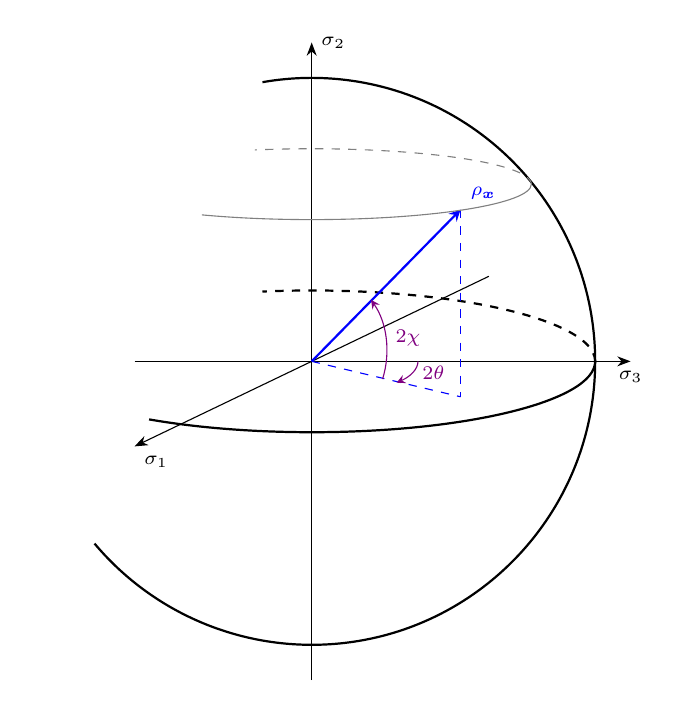
\begin{tikzpicture}[scale=0.9]
	%\draw[black, opacity=0.1] (-4.5,-4.5) grid (4.5,4.5);
	\draw[-Stealth] (2.5,1.2) -- (-2.5,-1.2)  node[below right]{$\sigma_1$};
	\draw[-Stealth] (0,-4.5) -- (0,4.5) node[right]{$\sigma_2$};
	\draw[-Stealth] (-2.5,0) -- (4.5,0) node[below]{$\sigma_3$};
	
	\coordinate (o) at (0,0);
	\coordinate (i) at (4,0);
	\coordinate (j) at (0,4);
	
	\coordinate (u) at (2.1,2.14);
	\coordinate (p) at (2.1, -0.5);
	\coordinate (v) at (3.4,0.5);
	
	% cercles
	\draw[thick] (4,0) arc [start angle=0, end angle =-140, radius = 4];
	\draw[thick] (4,0) arc [start angle=0, end angle =100, radius = 4];
	
	\draw[thick, dashed] (4,0) arc [start angle=0, end angle =100, radius = 4, y radius = 1];
	\draw[thick] (4,0) arc [start angle=0, end angle =-125, x radius = 4, y radius = 1];
	
	% droites
	\draw[-stealth,thick, blue] (0,0) -- (u) node[above right] {$\rho_{\x}$};
	\draw[dashed, blue] (u) -- (p);
	\draw[dashed, blue] (0,0) -- (p);
	
	%arc au point
	\draw[gray, dashed] (3.1,2.5) arc [start angle=0, end angle =105, radius = 3.1, y radius = 0.5];
	\draw[gray] (3.1,2.5) arc [start angle=0, end angle =-120, x radius = 3.1, y radius = 0.5];
	
	\draw[violet, -stealth] (1.5, 0) arc [start angle=0, end angle =-37, x radius = 1.5, y radius = 0.5] node[midway, right] {\scriptsize$2\theta$};    
	\draw[violet, -stealth] (1, -0.25) arc [start angle=-20, end angle =39, x radius = 1, y radius = 1.15] node[midway, right]{\scriptsize$2\chi$};
	
	% pos fixing
	\draw[white] (-4,0);
\end{tikzpicture}
	\caption{Sphère de Poincaré, blablabla}
	\label{fig:sphere2poincare}
\end{wrapfigure}

\par \noindent
où les $\sigma_i$ sont les matrices de Pauli :
\begin{align*}
	\sigma_1 &= \begin{pmatrix} 0 & 1 \\ 1 &  0 \end{pmatrix}  &
	\sigma_2 &= \begin{pmatrix} 0 & -i \\  i &  0 \end{pmatrix}  &
	\sigma_3 &= \begin{pmatrix} 1 & 0 \\ 0 & -1 \end{pmatrix}
\end{align*}
\skipl

Dans cette décomposition, la composante en $id$ est indépendante de $\x$ et peut donc être ignorée. Cela ne laisse qu'un vecteur (normé) de dimension 3 dont $2\theta$ et $2\chi$ correspondent aux coordonnées polaire conformément à la \Cref{fig:sphere2poincare} ci-contre.
\\ 
\\
La sphère alors obtenue, plus connu sous le nom de sphère de Poincaré, représente l'ensemble des états de polarisation possible pour un signal :
\\
À l'équateur, la polarisation est linéaire et $\theta$ pilote son orientation et plus $\rho_{\x}$ se rapproche des pôles, plus cette polarisation devient elliptique, jusqu'à devenir complètement circulaire, auquel cas $\theta$ devient insignifiant. 
Aussi, suivant le schéma \cref{fig:ellipse2polat}, l'hémisphère nord (resp. sud) correspond à des polarisations elliptiques anti-horaire (resp. horaire).

Le fait que ce soit deux fois les angles qui sont représentés tien naturellement compte des potentielles redondances dans les $(\theta,\chi)$. 
Par exemple si $\x$ à pour paramètre de polarisation instantanée $(\theta_0, \chi_0)$, alors par symétrie de l'ellipse, $(\theta_0+\pi, \chi_0)$ est aussi une représentation valide. Autre exemple, si $\chi_0 = \nicefrac{\pi}{4}$, alors la polarisation est circulaire et indépendant de $\theta_0$.
\\
Dans le deux cas, la représentation dans la sphère de Poincaré évite ces problèmes puisque, dans le premier cas $(2\theta_0, 2\chi_0)$ et $(2\theta_0+2\pi, 2\chi_0)$ représente le même point, et dans le second, le point associé à $2\chi_0=\nicefrac{\pi}{2}$ (pôle nord) est indépendant du choix de $\theta_0$.
\\

\begin{figure}[h]
	\includegraphics[width=0.8\textwidth]{fig/placeholder}
	\caption{Représentation des paramètres de polarisation instantanée associés à chaque point de la sphère de Poincaré.}
\end{figure}


Pour interpréter la formule \eqref{eq:phases_p-cyc_2var} de la phase géométrique prenons un exemple. Si $\chi$ et $\theta$ sont telle que :
\begin{align*}
	2\theta(t_0) &= 0  &  2\theta(t) &= 2\pi  &  \chi(s) &= \chi_0
\end{align*}
Alors décrit un chemin horizontale sur la sphère, $\rho_{\x}(t_0) = \rho_{\x}(t)$ et sa phase géométrique s'écrit :
\begin{align*}
	\phaseg(\x, t_0, t) = -\int_{t_0}^t \theta'(s) \sin 2\chi(s) ds &= - \sin 2\chi_0 \int_{t_0}^t \theta'(s) ds \\
	&= - \sin 2\chi_0 \big( \theta(t) - \theta(t_0)\big) \\
	&= - \pi\sin 2\chi_0
\end{align*}

Cette formule est très proche de la formule de d'air de la calotte entouré par $\rho_{\x}$, à savoir%\footnote{\itshape
	%La formule se trouve sans mal sur \href{https://fr.wikipedia.org/wiki/Calotte_sph%C3%A9rique#Aire}{Wikipédia}. Dans le lien donné, la formule est fait apparaître un cos, ce qui est dû au choix de convention sur l'angle décrit par $\chi_0$ ($=\nicefrac{\pi}{2} - \theta$ sur Wikipédia)} 
 :
\[\mathcal{A}ire = 2\pi - 2\pi \sin(2\chi_0)\]
Pour la faire clairement apparaître, il suffit de noter que $\phaseg$ étant une phase, elle est définie modulo $2\pi$ et à un facteur 2 près, elle s'écrit :
\begin{align*}
	{\color{white}bbbbbbbbbbbbbbbbbbbbbbbbbbbbbbb}\phaseg(\x, t_0, t) &\equiv 2\pi - \pi\sin 2\chi_0   &  &[2\pi] {\color{white}bbbbbbbbbbbbbbbbbbbbbbbbbbbbbbb} \\
	 &\equiv \frac{1}{2}\big( 4\pi - 2\pi\sin 2\chi_0 \big)    &  &[2\pi] 
\end{align*}

Soit la moitié de l'aire de la calotte au dessus du chemin tracé par $\rho_{\x}$ plus $2\pi$. Une fois n'est pas coutume, ca va toujours pas et j'ai envie de me foutre en l'air atm





\subsection{Généralisation en plus haute dimension} \label{subsec:aller_plus_loin}

\begin{itemize}
	
	\item Différentes écritures du bivarié pour différentes généralisation :
	
	\item Les quaterions on passe vites parce que ca se généralise très mal, Lefevre a a parlée, ca mène aux algèbres Clifford : trop de contrainte sur les dimensions des signaux
	
	\item En terme d'expo de matrice ? Lefevre \cite[sec. I.3]{lefevre_polarization_2021} l'a fait en trivarié mais au delà, y'a plus vraiment de choix remarquable de base pour $\mathfrak{u}(n)$
	
	\item En augmentant la taille de la matrice de rotation ? Lilly \cite{lilly_modulated_2011} l'a fait en trivarié et mais là encore, en terme de généralisation c'est pas si dingue parce que la matrice de rotation est pas calculable.
	
	\item Dans tout ça, on ratte le plus important : La phase géo est invariante par transfo de jauge, donc il faut faut faire apparaître $\PC{n-1}$ dans la décomposition.
	
	\item et en fait, c'est le cas en bivarié car $\PC{1}\cong \S{2}$ !
	
	\item $\PC{n-1}$ oui mais il faut pas non plus regarder que la projection parce qu'on perd toute les phases dans ce cas.
	
	\item Le bon compromis c'est les variétés fibrées : on est dans $\PC{n-1}$ mais on garde les phases dans les fibres.
	
	\item D'autant plus que ça à déjà était fait en physique et c'est vraiment concluant... (transition vers la grande partie suivante.)
	
\end{itemize}

Au niveau des ensembles, décomposer un signal multivarié complexe en paramètre d'amplitude, phase et polarization instantanée, revient à décomposer $\C^n$ en un produit de trois ensembles. Pour cela, un vecteur de $\C^n$ est vu comme la donné d'une direction, \ie~un élément de la sphère unité $S^{2n-1}\subset\C^n$, et d'une norme, de sorte que :
\[\C^n \cong \R^{+_*} \times S^{2n-1}\]
\\
Les éléments de $\R^{+_*}$ s'interprète naturellement comme l'amplitude instantanée du signal et pour faire apparaître sa phase, $S^{2n-1}$ est lui-même décomposé de sorte à faire apparaître $\U{1}$, donnant :
\[\C^n \cong \R^{+_*} \times \U{1} \times S^{2n-1}/\U{1}\]
Le quotient restant n'est autre que l'espace projectif complexe de dimension (complexe) $n-1$, noté $\PC{n-1}$. Sa construction sera détaillée dans la \cref{part:phase_geo} suivante.
\\

Pour motiver d'autant plus cette décomposition, la projection $\rho : \x \lr \congu{\x}\,^t\x / \|\x\|^2$, qui s'est avérée fort instructive, peut être vue comme une projection sur l'espace complexe en cela qu'elles sont toutes deux invariantes par transformation de jauge\footnote{\itshape
	Pour être précis, c'est le premier théorème d'isomorphisme assure $\rho(\C^n) \cong\PC{n-1}$ sont en bijection et de même structure.}.
En particulier, si $n=2$, $\PC{1}\cong S^{2}$, soit exactement l'espace de représentation des $\rho_{\x}$ dans la section précédente.




%%%% ANNEXES %%%%



\begin{annexe}

\section{Annexes}

\subsection{Compléments sur l'analyse temps-fréquence}\label{ann:complement_t-f}

\subsubsection{Un mot sur la notion de fréquence instantanée \thoughts{(nécessaire?)}}\label{ann:freq_instant}

\subsubsection{Formalisme dernière la transformée en SA}\label{ann:transfo_SA}

\subsubsection{Lien avec le théorème de Bedrosian}\label{ann:bedrosian}

\subsection{Compléments sur les signaux AM-FM-PM}\label{ann:AM-FM-PM}

\subsubsection{Construction détaillée des signaux AM-FM-PM \thoughts{(nécessaire?)}}\label{ann:construc_AM-FM-PM}

\begin{itemize}
	
	\item Signal polarisé classique ($\theta,\chi$ constants)
	
	\item Transformé en SA avec les hypothèse de Bedrosian 
	
	\item Définition général en faisant dépendre $\theta / \chi$ du temps
	
	\item Paramètre de Polar sur la sphère de Poincaré
	
\end{itemize}


\subsubsection{Démonstrations}\label{ann:demo_phases_2var}

\begin{demo}[de la formule \eqref{eq:phased_2var}, \cref{prop:phases_2var}]
	Par souci de lisibilité, on note $\ \mathcal{U} = R_{\theta} \begin{pmatrix} \cos\chi \\ -i\sin\chi \end{pmatrix} = \begin{pmatrix} \cos\theta(t) \cos\chi(t) + i\sin\theta(t) \sin\chi(t) \\ \sin\theta(t) \cos\chi(t) - i\cos\theta(t) \sin\chi(t) \end{pmatrix}$, de sorte que la dérivée de $\ \x=ae^{i\varphi}\mathcal{U}\ $ s'écrive :
	\[\dot{\x} = a'e^{i\varphi}\mathcal{U} + ia\varphi'e^{i\varphi} \mathcal{U} + ae^{i\varphi}\theta'\begin{pmatrix} -\sin\theta \cos\chi + i\cos\theta \sin\chi \\ \cos\theta \cos\chi + i\sin\theta \sin\chi \end{pmatrix} + ae^{i\varphi}\chi'\begin{pmatrix} -\cos\theta \sin\chi + i\sin\theta \cos\chi \\ -\sin\theta \sin\chi - i\cos\theta \cos\chi \end{pmatrix}\]
	\\
	Les vecteurs des deux derniers membres s'expriment en fonction des composantes $\ \mathcal{U}_{1,2}\ $ de $\ \mathcal{U}$ :
	\begin{align*}
		\begin{pmatrix} -\sin\theta \cos\chi + i\cos\theta \sin\chi \\ \cos\theta \cos\chi + i\sin\theta \sin\chi \end{pmatrix} &= \begin{pmatrix} -\mathcal{U}_2 \\ \mathcal{U}_1 \end{pmatrix}  &
		\begin{pmatrix} -\cos\theta \sin\chi + i\sin\theta \cos\chi \\ -\sin\theta \sin\chi - i\cos\theta \cos\chi \end{pmatrix} &= i\begin{pmatrix} \congu{\mathcal{U}}_2 \\ -\congu{\mathcal{U}}_1 \end{pmatrix}
	\end{align*}
	\\
	Le produit hermitien $\langle \dot{\x}, \x \rangle$ s'écrit alors :
	\begin{align*}
		\langle \dot{\x}, \x \rangle 
		&= \left\langle a'e^{i\varphi}\mathcal{U} + ia\varphi'e^{i\varphi} \mathcal{U} + ae^{i\varphi}\theta'\begin{pmatrix} -\mathcal{U}_2 \\ \mathcal{U}_1 \end{pmatrix} + iae^{i\varphi}\chi'\begin{pmatrix} \congu{\mathcal{U}}_2 \\ -\congu{\mathcal{U}}_1 \end{pmatrix}, ae^{i\varphi}\mathcal{U} \right\rangle \\
		&= \left\langle a'\mathcal{U} + ia\varphi' \mathcal{U} + a\theta'\begin{pmatrix} -\mathcal{U}_2 \\ \mathcal{U}_1 \end{pmatrix} + ia\chi'\begin{pmatrix} \congu{\mathcal{U}}_2 \\ -\congu{\mathcal{U}}_1 \end{pmatrix}, a\mathcal{U} \right\rangle \\
		&= aa' \big\langle \mathcal{U}, \mathcal{U}\big\rangle  + ia^2\varphi' \big\langle \mathcal{U}, \mathcal{U}\big\rangle  + a^2\theta'\left\langle \begin{pmatrix} -\mathcal{U}_2 \\ \mathcal{U}_1 \end{pmatrix}, \mathcal{U} \right\rangle + ia^2\chi'\left\langle \begin{pmatrix} \congu{\mathcal{U}}_2 \\ -\congu{\mathcal{U}}_1 \end{pmatrix}, \mathcal{U} \right\rangle
	\end{align*}
	où les deux derniers produits hermitiens donnent :
	\begin{align*}
		\left\langle \begin{pmatrix} -\mathcal{U}_2 \\ \mathcal{U}_1 \end{pmatrix}, \mathcal{U} \right\rangle &= -\mathcal{U}_2\congu{\mathcal{U}}_1 + \mathcal{U}_1\congu{\mathcal{U}}_2 \\
		&= 2i\Im m\big(\mathcal{U}_1 \congu{\mathcal{U}}_2\big) \\
		&= 2i\Im m\Big(\big( \cos\theta \cos\chi + i \sin\theta \sin\chi \big) \big( \sin\theta \cos\chi + i \cos\theta \sin\chi \big)\Big) \\
		&= 2i\big(\cos^2\theta \cos\chi \sin\chi + \sin^2\theta \sin\chi \cos\chi \big) \\
		&= 2i \cos\chi \sin\chi \\
		&= i\sin2\chi 
		\\ \\
		\left\langle \begin{pmatrix} \congu{\mathcal{U}}_2 \\ -\congu{\mathcal{U}}_1 \end{pmatrix}, \mathcal{U} \right\rangle &= \congu{\mathcal{U}_2\mathcal{U}_1} - \congu{\mathcal{U}_1\mathcal{U}_2} = 0
	\end{align*}
	\\
	D'où, sachant que $\ \|\x\|^2=a^2\ $ et $\ \|\mathcal{U}\|=1$, la formule :
	\begin{align*}
		\frac{\Im m\big\langle \dot{\x}, \x\big\rangle}{\|\x\|^2} &= \frac{1}{a^2}\Im m\Big(aa' \big\langle \mathcal{U}, \mathcal{U}\big\rangle  + ia^2\varphi' \big\langle \mathcal{U}, \mathcal{U}\big\rangle + ia^2\theta' \sin2\chi \Big) \\
		&= \frac{1}{a^2} \Big( a^2\varphi' \|\mathcal{U}\|^2 + a^2\theta' \sin2\chi \Big) \\
		&= \varphi' + \theta' \sin2\chi
	\end{align*}
\end{demo}

\begin{demo}[de la formule \eqref{eq:phaset_2var}, \cref{prop:phases_2var}]
	Pour la phase totale, on note cette fois $\mathcal{V} = \begin{pmatrix} \cos\chi \\ -i\sin\chi \end{pmatrix}$ et on a :
	\begin{align*}
		\big\langle \x(t), \x(t_0)\big\rangle &= \Big\langle a(t)e^{i\varphi(t)}R_{\theta(t)}\mathcal{V}(t), a(t_0)e^{i\varphi(t_0)}R_{\theta(t_0)}\mathcal{V}(t_0) \Big\rangle \\
		&= a(t)e^{i\varphi(t)} a(t_0)e^{-i\varphi(t_0)} \Big\langle R_{\theta(t)}\mathcal{V}(t), R_{\theta(t_0)}\mathcal{V}(t_0) \Big\rangle \\
		%&= a(t_0)a(t)e^{i(\varphi(t_0)-\varphi(t))}\Big\langle \mathcal{V}(t_0), R_{\theta(t_0)}^{-1}R_{\theta(t)}\mathcal{V}(t) \Big\rangle \\
		&= a(t_0)a(t)e^{i(\varphi(t)-\varphi(t_0))}\Big\langle R_{\theta(t)- \theta(t_0)}\mathcal{V}(t), \mathcal{V}(t_0) \Big\rangle
	\end{align*}
	Pour alléger les notations, on note $\ \Delta y =y(t)-y(t_0)$, $\ y_1=y(t_0)\ $ et $\ y_2=(t)\ $ pour $\ y=\varphi,\theta,\chi$. Le produit hermitien à droite s'écrit alors :
	\begin{align*}
		\Big\langle R_{\Delta\theta}\mathcal{V}(t), \mathcal{V}(t_0) \Big\rangle &=   \Big(\cos\Delta\theta \cos\chi_2 + i\sin\Delta\theta \sin\chi_2 \qquad \sin\Delta\theta \cos\chi_2 - i\cos\Delta\theta \sin\chi_2\Big) \begin{pmatrix} \cos\chi_1 \\ i\sin\chi_1 \end{pmatrix} \\
		&= \cos\chi_1\Big(\cos\Delta\theta \cos\chi_2 + i\sin\Delta\theta \sin\chi_2\Big) + i\sin\chi_1\Big(\sin\Delta\theta \cos\chi_2 - i\cos\Delta\theta \sin\chi_2\Big) \\
		&= \cos\Delta\theta \Big(\cos\chi_1 \cos\chi_2 + \sin\chi_1 \sin\chi_2\Big) + i\sin\Delta\theta \Big( \cos\chi_1 \sin\chi_2 + \sin\chi_1\cos\chi_2\Big) \\
		&= \cos\Delta\theta \cos\Delta\chi + i\sin\Delta\theta \sin(\chi_1+\chi_2)
	\end{align*}
	\\
	D'où la phase totale :
	\begin{align*}
		\phaset(\x) = \arg\big\langle \x(t), \x(t_0)\big\rangle &= \arg\left( a(t_0)a(t)e^{i(\varphi(t) - \varphi(t_0))}\Big( \cos\Delta\theta \cos\Delta\chi + i\sin\Delta\theta \sin(\chi_1+\chi_2) \Big) \right) \\
		&= \varphi(t) - \varphi(t_0) + \arg\Big( \cos\Delta\theta \cos\Delta\chi + i\sin\Delta\theta \sin(\chi_1+\chi_2) \Big)
	\end{align*}
	et l'argument restant s'écrit comme une arctangente, donnant :
	\begin{align*}
		\phaset(\x) &= \varphi(t)-\varphi(t_0) + \arctan\frac{\sin\Delta\theta \sin(\chi_1+\chi_2)}{\cos\Delta\theta \cos\Delta\chi} \\
		&= \varphi(t)-\varphi(t_0) + \arctan \left( \tan\Delta\theta\frac{\sin(\chi_1+\chi_2)}{\cos\Delta\chi} \right) \\
		&= \cdots
	\end{align*}
\end{demo}
\skipl


\subsection{Lien entre Poincaré et Bloch}

\subsubsection{Lien entre les deux types de signaux}

Soit le signal :
\[\x_B(\varphi, \theta, \chi) = e^{i\varphi} \begin{pmatrix}
	\cos \chi/2 \\ e^{i\theta}\sin\chi/2\end{pmatrix}\]
Pour le réécrire en terme de vecteur AM-FM-PM, il faut faire apparaître une matrice de rotation, matrice qui est diagonalisable dans $\C^{n\times n}$ via la relation :
\begin{align*}
	&\begin{pmatrix} 
		\cos \alpha & -\sin \alpha \\ 
		\sin\alpha & \cos\alpha 
	\end{pmatrix} = \frac{1}{2} \begin{pmatrix} 
		1 & -1 \\ i & i
	\end{pmatrix}\begin{pmatrix} 
		e^{-i\alpha} & 0 \\ 
		0 & e^{i\alpha} 
	\end{pmatrix}\begin{pmatrix} 
		1 & -i \\ -1 & -i
	\end{pmatrix}\\
	&\Llr\quad \begin{pmatrix} 
		1 & -i \\ -1 & -i
	\end{pmatrix}\begin{pmatrix} 
		\cos \alpha & -\sin \alpha \\ 
		\sin\alpha & \cos\alpha 
	\end{pmatrix} \begin{pmatrix} 
		1 & -1 \\ i & i
	\end{pmatrix} = 2 \begin{pmatrix} 
		e^{-i\alpha} & 0 \\ 
		0 & e^{i\alpha} 
	\end{pmatrix}
\end{align*}
\\
Cela permet d'écrire :
\begin{align*}
	\x_B(\varphi, \theta, \chi) &= e^{i\varphi} e^{i\theta/2}\begin{pmatrix}
			e^{-i\theta/2} & 0 \\
			0 & e^{i\theta/2}
		\end{pmatrix}\begin{pmatrix} 
			\cos \chi/2 \\ 
			\sin \chi/2 
		\end{pmatrix} \\
		&= \frac{1}{2}e^{i\varphi} e^{i\theta/2}\begin{pmatrix} 
			1 & -i \\
			-1 & -i
		\end{pmatrix}\begin{pmatrix} 
			\cos \theta/2 & -\sin \theta/2 \\ 
			\sin \theta/2 & \cos \theta/2 
		\end{pmatrix} \begin{pmatrix} 
			1 & -1 \\ i & i
		\end{pmatrix}\begin{pmatrix} 
			\cos \chi/2 \\ 
			\sin\chi/2
		\end{pmatrix} \\
		&= \frac{\sqrt{2}}{2}e^{i(\varphi + \theta/2)}U R_{\theta/2} \begin{pmatrix} 
			\cos \chi/2 - \sin\chi/2 \\ 
			i\big(\cos\chi/2 + \sin\chi/2\big)
		\end{pmatrix}   & &\text{où }\quad U = \frac{\sqrt{2}}{2}\begin{pmatrix} 
		1 & -i \\ -1 & -i
		\end{pmatrix}\in \U{2} \\
\end{align*}
\\
Ensuite, pour réduire les sommes dans le vecteur de droite, on a rappel les formules :
\begin{align*}
	\cos\left( \frac{\pi}{2} \pm \alpha\right) &= \frac{\sqrt{2}}{2}\big( \cos\alpha \mp \sin \alpha \big) & \sin\left( \frac{\pi}{2} \pm \alpha\right) &= \frac{\sqrt{2}}{2}\big( \cos\alpha \pm \sin \alpha \big)
\end{align*}
\\ 
On a donc deux choix pour chaque composante du vecteur mais celle avec un signe moins son préférable sachant que : 
\begin{align*}
	\cos\left( \frac{\pi}{2} - \alpha\right) &= \sin(\alpha) &  \sin\left( \frac{\pi}{2} - \alpha\right) &= \cos(\alpha)
\end{align*}
\\
On choisi donc la seconde formule pour la première composante et la premier pour la seconde composante, donnant :
\begin{align*}
	\x_B(\varphi, \theta, \chi) &= \frac{\sqrt{2}}{2}e^{i(\varphi + \theta/2)}U R_{\theta/2} \begin{pmatrix} 
		\cos \chi/2 - \sin\chi/2 \\ 
		i\big(\cos\chi/2 + \sin\chi/2\big)
	\end{pmatrix} \\
	&= e^{i(\varphi + \theta/2)}U R_{\theta/2} \begin{pmatrix} 
		\sin\left( \frac{\pi}{2} - \chi/2\right) \\ 
		i\cos\left( \frac{\pi}{2} - \chi/2\right)
	\end{pmatrix} \\
	&= e^{i(\varphi + \theta/2)}U R_{\theta/2} \begin{pmatrix} 
		\cos \chi/2 \\ 
		i\sin \chi/2
	\end{pmatrix}
\end{align*}
\\
Ne reste alors plus qu'à ajuster les signes pour obtenir une écriture de signal $\x_P$ AM-FM-PM :
\begin{align*}
	\x_B(\varphi, \theta, \chi) &= e^{i(\varphi + \theta/2)}U R_{\theta/2} \begin{pmatrix} 
		\cos \chi/2 \\ 
		i\sin \chi/2
	\end{pmatrix} \\
	&= U e^{i(\varphi + \theta/2)} R_{\theta/2} \begin{pmatrix} 
		\cos (-\chi/2) \\ 
		-i\sin (-\chi/2)
	\end{pmatrix}
\end{align*}
En somme :
\begin{align} \label{eq:bloch2poinca}
	\x_B(\psi, \alpha, \beta) &= U \x_P(\psi + \alpha/2, \alpha/2, -\beta/2)  & 
	\x_P(\varphi, \theta, \chi) = U^\dagger 	\x_B(\varphi-\theta, 2\theta, -2\chi)	
\end{align}
\skipl 



\subsubsection{Lien entre les projections}

Avec la formule \eqref{eq:bloch2poinca} ci-dessus, on a :

\begin{align}
	\rho_B(\alpha, \beta) &= U \rho_P(\alpha/2, -\beta/2)U^\dagger  & 
	\rho_P(\theta, \chi) &= U^\dagger \rho_B(2\theta, -2\chi) U
	%\\ \Llr\ \rho_B(\alpha, \beta) U &= U \rho_P(\alpha/2, -\beta/2) & \Llr\ \rho_P(\theta, \chi) U^\dagger &= U^\dagger \rho_B(2\theta, -2\chi) 
\end{align}
\\
Mais on a aussi, dans la base Pauli :
\begin{align*}
	\sigma_1 &= \begin{pmatrix} 0 & 1 \\ 1 &  0 \end{pmatrix}  &
	\sigma_2 &= \begin{pmatrix} 0 & -i \\  i &  0 \end{pmatrix}  &
	\sigma_3 &= \begin{pmatrix} 1 & 0 \\ 0 & -1 \end{pmatrix}
\end{align*}
les expressions :
\begin{align*}
	\rho_{P}(\theta, \chi) &= \frac{1}{2} \Big( id + \sin(2\theta) \cos(2\chi) \sigma_1 - \sin (2\chi) \sigma_2 + \cos(2\theta) \cos(2\chi) \sigma_3 \Big) \\ 
	\rho_{B}(\alpha, \beta) &= \frac{1}{2} \Big( id + \cos(\alpha) \sin(\beta) \sigma_1 + \sin(\alpha) \sin(\beta) \sigma_2 + \cos (\beta) \sigma_3 \Big)
\end{align*}
\skipl

Pour les lier, on pose $\ 2\theta = \nicefrac{\pi}{2} - \alpha\ $ et $\ 2\chi = \nicefrac{\pi}{2} - \beta$, donnant :
\begin{align*}
\rho_P(\theta, \chi) - id 
	&= \sin(\nicefrac{\pi}{2} - \alpha) \cos(\nicefrac{\pi}{2} - \beta) \sigma_1 - \sin (\nicefrac{\pi}{2} - \beta) \sigma_2 + \cos(\nicefrac{\pi}{2} - \alpha) \cos(\nicefrac{\pi}{2} - \beta) \sigma_3 \\
	&= \cos(\alpha) \sin(\beta) \sigma_1 - \cos (\beta) \sigma_2 + \sin(\alpha) \sin(\beta) \sigma_3
\end{align*}
\\
Ce qui sous forme matricielle se réécrit :
\[\begin{pmatrix}
	\sin(2\theta) \cos(2\chi) \\ -\sin (2\chi) \\ \cos(2\theta) \cos(2\chi)
\end{pmatrix} = \begin{pmatrix}
	\cos(\alpha) \sin(\beta) \\ -\cos (\beta) \\ \sin(\alpha) \sin(\beta)
\end{pmatrix} = \begin{pmatrix}
	1 & 0 & 0 \\ 0 & 0 & -1 \\ 0 & 1 & 0
\end{pmatrix}\begin{pmatrix}
	\cos(\alpha) \sin(\beta) \\ \sin(\alpha) \sin(\beta) \\ \cos (\beta)
\end{pmatrix}\]
\\
Donc la passage de $\rho_B$ à $\rho_S$ se fait via un changement et d'angle et une rotation de $\nicefrac{\pi}{2}$ autour de $\sigma_1$.
\\

Même calcul, cette fois, en partant de \eqref{eq:bloch2poinca} :
\begin{align*}
	2\rho_P(\theta, \chi) &= 2U^\dagger \rho_B(2\theta, -2\chi) U \\
	&= U^\dagger \Big( id + \cos(2\theta) \sin(-2\chi) \sigma_1 + \sin(2\theta) \sin(-2\chi) \sigma_2 + \cos (-2\chi) \sigma_3 \Big) U \\
	&= id - \cos(2\theta) \sin(2\chi) U^\dagger \sigma_1 U - \sin(2\theta) \sin(2\chi) U^\dagger \sigma_2 U + \cos (2\chi) U^\dagger \sigma_3 U
\end{align*}
avec :
\begin{align*}
	U^\dagger \sigma_1 U &= \frac{1}{2} \begin{pmatrix} 
		1 & -1 \\ i & i
	\end{pmatrix} \begin{pmatrix} 
		0 & 1 \\ 1 &  0 
	\end{pmatrix} \begin{pmatrix} 
		1 & -i \\ -1 & -i
	\end{pmatrix} = \frac{1}{2} \begin{pmatrix} 
		-2 & 0 \\ 0 & 2
	\end{pmatrix} = -\sigma_3 \\
	U^\dagger \sigma_2 U &= \frac{1}{2} \begin{pmatrix} 
		1 & -1 \\ i & i
	\end{pmatrix} \begin{pmatrix} 
		0 & -i \\  i &  0 
	\end{pmatrix} \begin{pmatrix} 
		1 & -i \\ -1 & -i
	\end{pmatrix} = \frac{1}{2} \begin{pmatrix} 
		0 & -2 \\ -2 & 0
	\end{pmatrix} = -\sigma_1 \\
	U^\dagger \sigma_3 U &= \frac{1}{2} \begin{pmatrix} 
		1 & -1 \\ i & i
	\end{pmatrix}  \begin{pmatrix} 
		1 & 0 \\ 0 & -1 
	\end{pmatrix} \begin{pmatrix} 
		1 & -i \\ -1 & -i
	\end{pmatrix} = \frac{1}{2} \begin{pmatrix} 
		0 & -2i \\ 2i & 0
	\end{pmatrix} = \sigma_2
\end{align*}
\\
Qui donne :
\begin{align*}
	2\rho_P(\theta, \chi) &= id - \cos(2\theta) \sin(2\chi) U^\dagger \sigma_1 U - \sin(2\theta) \sin(2\chi) U^\dagger \sigma_2 U + \cos (2\chi) U^\dagger \sigma_3 U \\
	&= id + \cos(2\theta) \sin(-2\chi) \sigma_3 + \sin(2\theta) \sin(-2\chi)  \sigma_1 + \cos (-2\chi) \sigma_2 \\
	&= id + \sin(2\theta) \sin(2\chi)  \sigma_1 + \cos (2\chi) \sigma_2 + \cos(2\theta) \sin(2\chi) \sigma_3
\end{align*}
\\ 
Le tout reste cohérent et avec les notations :
\begin{align*}
	w_P(\theta, \chi) &= \begin{pmatrix}
		\sin(\theta) \cos(\chi) \\ -\sin (\chi) \\ \cos(\theta) \cos(\chi)
	\end{pmatrix}  &   w_B\big( \alpha, \beta \big) = \begin{pmatrix}
		\cos(\alpha) \sin(\beta) \\ \sin(\alpha) \sin(\beta) \\ \cos (\beta)
	\end{pmatrix}
\end{align*}
Cela devient :
\[w_P(2\theta, 2\chi) = \begin{pmatrix}
	1 & 0 & 0 \\ 0 & 0 & -1 \\ 0 & 1 & 0
\end{pmatrix} w_B\big( (\nicefrac{\pi}{2}-\theta ), \big(\nicefrac{\pi}{2}-\chi) \big)\]
\skipl 



\subsubsection{Transformation de phases}

Première chose, le produit hermitien est invariant par $U\in\U{2}$ (si si). Ainsi :
\[\big\langle U\x(t_0), U\x(t) \big\rangle = \big\langle \x(t_0), \x(t) \big\rangle\]
\[\big\langle (U\x)', U\x \big\rangle = \big\langle U\x', U\x \big\rangle = \big\langle \x', \x \big\rangle\]
\\
Ainsi, en utilisant les formules \eqref{eq:phaset_2var} et \eqref{eq:bloch2poinca}, on a :
\begin{align*}\phaset \big(\x_B(\psi, \alpha, \beta) \big) &= \phaset \big(\x_P(\psi + \alpha/2, \alpha/2, -\beta/2) \big) \\
	&= \big( \psi + \alpha/2 \big)(t) - \big( \psi + \alpha/2 \big)(t_0) - \arctan\left( \tan \frac{\Delta\theta}{2} \frac{ \tan 2\beta(t_0)+\tan 2\chi(t)}{1 + \tan 2\beta(t_0)\tan 2\beta(t)}\right)
\end{align*}
Mais avec un calcul immédiat, on a aussi :
\[aoerinagrqobne\]
\\
Avec la formule de la phase dynamique dans Poincaré \eqref{eq:phased_2var}, on a :
\begin{align*}
	%\phaset \big(\x_B(\psi, \alpha, \beta) \big) &= \phaset \big(\x_P(\psi + \alpha/2, \alpha/2, -\beta/2) \big) 
	%\\ \\
	\phased \big(\x_B(\psi, \alpha, \beta) \big) &= \Im m \int_{t_0}^t \left\langle \frac{d}{ds}\x_B(\psi, \alpha, \beta), \x_B(\psi, \alpha, \beta) \right\rangle ds \\
	&= \Im m \int_{t_0}^t \left\langle \frac{d}{ds}\x_P(\psi + \alpha/2, \alpha/2, -\beta/2), \x_P(\psi + \alpha/2, \alpha/2, -\beta/2) \right\rangle ds \\
	&= \phased \big( \x_P(\psi + \alpha/2, \alpha/2, -\beta/2) \big) \\
	&= \psi(t) + \alpha(t)/2 - \big( \psi(t_0) + \alpha(t_0)/2 \big) - \int_{t_0}^t \frac{\alpha'(s)}{2} \sin \big( -2\beta(s)/2 \big) ds \\
	&= \psi(t) - \psi(t_0) + \frac{\alpha(t) - \alpha(t_0)}{2} + \frac{1}{2} \int_{t_0}^t \alpha'(s)\sin \beta(s) ds
\end{align*}
\\
Mais dans le même temps, si on calcul la phase dynamique de $\x_B$, on tombe cette fois sur :
\begin{align*}
	\phased\big(\x_B(\psi, \alpha, \beta) \big) &= \psi(t) - \psi(t_0) +  \int_{t_0}^t \alpha'(s) \frac{1 - \cos\beta(s)}{2}ds \\
	&= \psi(t) - \psi(t_0) + \frac{\alpha(t) - \alpha(t_0)}{2}- \frac{1}{2} \int_{t_0}^t \alpha'(s) \cos\beta(s) ds 
\end{align*}
Auquel cas :
\begin{align*}
	\phased\big(\x_S(\varphi, \theta, \chi) \big) &= \phased\big(\x_B(\varphi-\theta, 2\theta, -2\chi) \big) \\
	&= \varphi(t) - \theta(t) - \big( \varphi(t_0) - \theta(t_0) \big) + \frac{1}{2} \int_{t_0}^t 2\theta' (1 - \cos2\chi)ds \\
	&= \varphi(t) - \varphi(t_0) - \big( \theta(t) - \theta(t_0) \big) + \int_{t_0}^t \theta' (1 - \cos2\chi)ds \\
	&= \varphi(t) - \varphi(t_0) - \big( \theta(t) - \theta(t_0) \big) + \big( \theta(t) - \theta(t_0) \big) - \int_{t_0}^t \theta' \cos2\chi ds \\
	&= \varphi(t) - \varphi(t_0) - \int_{t_0}^t \theta' \cos2\chi ds
\end{align*}
Ce qui voudrait dire que :
\[\phased\big(\x_S(\varphi, \theta, \chi) \big) = \varphi(t) - \varphi(t_0) + \int_{t_0}^t \theta' \sin2\chi ds = \varphi(t) - \varphi(t_0) - \int_{t_0}^t \theta' \cos2\chi ds\]
... bizarre


\end{annexe}
%\begin{annexe}\section{Annexes}

\subsection{Compléments sur l'analyse temps-fréquence}\label{ann:complement_t-f}

Cette annexe est une adaptation 

\subsubsection{\wip Formalisme derrière la transformée en SA ou le problème de signaux réels et comment le résoudre}\label{sec:transfo_SA}

D'abord, du point de vue de l'analyse temps-fréquence, les signaux réels sont problématiques car leur spectre sont à symétrie hermitienne et leur  densité spectrale symétrique :
\begin{align*}
	\forall t\in\R,\ x(t)\in\R \quad &\Lr \quad \forall \nu\in\R,\ \fou{x}(-\nu) = \congu{\fou{x}(\nu)} \\
	&\Lr \quad \forall \nu\in\R,\ \densis(-\nu) = \densis(\nu)
\end{align*}
\skipl \\
Comme mentionné plus haut, cela implique que la fréquence moyenne de tout signal réel est nulle (intégrale d'une fonction impaire). Ce qui, en plus de ne pas être très instructif, n'est pas cohérent avec l'interprétation physique qu'on voudrait faire cette moyenne. Par exemple, si $\densis$ prend la forme ci-dessous (\cref{fig:densi_spec_sym}), alors il serait plus naturelle de demander à ce que la fréquence moyenne se trouve autour de \textbf{1,4}. De même, la largeur de bande spectrale ne correspond plus à l'étalement de chaque gaussienne, mais plutôt à leur espacement.
\\
\begin{figure}[h]\centering
	\includegraphics[width=0.9\textwidth]{fig/part-1/densi_spec_sym}
	\caption{Exemple de densité spectrale d'un signal réel \textbf{ESP A 1,4}}
	\label{fig:densi_spec_sym}
\end{figure}
\\
Même problème avec la covariance : sachant l'égalité des deux notions de fréquences moyenne (\cref{eq:esp_freq}, \cref{prop:mom_freq}), on peut définir la covariance temps-fréquence d'un signal $x$ par :
\begin{align*}
	\text{Cov}(x) \defeq \text{Cov}\big(t,\phi'(t) \big) 
	&= \esp[\densit]{t\phi'(t)} - \esp[\densit]{t} \esp[\densit]{\phi'(t)} \\
	&= \esp[\densit]{t\phi'(t)} - \esp[\densit]{t} \esp[\densis]{\nu}	
\end{align*}
\\
Ce coefficient est sensé mesurer une corrélation entre l'évolution d'un signal au cours du temps avec ses fréquences. S'il est réel, alors  $\text{Cov}(x)$ sera toujours nulle ; de là à en conclure que la fréquence instantanée de n'importe quel signal (réel) est toujours décorrélée du temps serait, pour le moins, insatisfaisant.
\\

Pour résoudre le problème, une méthode consiste à construire un nouveau signal $\SA{x}$ en supprimant les fréquences négatives de $x$ :
\[\mathcal{F}\big[\SA{x}\big] = 2\one_{\R^+}\fou{x}\]
où $\one_E$ est la fonction indicatrice sur l'ensemble $E$ et où le facteur 2 assure la conservation de l'énergie du signal. Cela mène à la définition :

\begin{definition}[Transformée de Hilbert et en SA]\label{def:transfo_sa&hilbert}
	On appelle \emph{transformé de Hilbert de} $x$, l'application :
	\begin{equation}\label{eq:transfo_Hilb}
		\mathcal{H}[x] :\ \begin{aligned} 
			\R \quad &\lr\qquad\quad \C \\	
			t\quad &\longmapsto\ \frac{1}{\pi}\fint_\R \frac{x(s)}{t-s}ds %=  \frac{1}{\pi}\left(\vpC\right)*x
		\end{aligned}
	\end{equation}
	où l'intégrale barré représente la \emph{valeur principale de Cauchy} (voir \cref{ann:transfo_SA} pour plus de détail) :
	\begin{align*}
		\fint_\R \frac{x(s)}{t-s}ds &\defeq \lim_{\varepsilon\lr0^+} \int_{-\infty}^{-\varepsilon} \frac{\varphi(t)}{t}dt + \int_{+\varepsilon}^{+\infty} \frac{\varphi(t)}{t}dt 
		%\\ &= \int_0^{+\infty} \frac{\varphi(t) - \varphi(-t)}{t}dt
	\end{align*}
	Avec, on définit la \emph{transformée en signal analytique} (SA) de tout signal $x$ comme l'unique application $\SA{x}$ telle que $\ \Fou{\SA{x}\big.}= 2\one_{\R^+}\fou{x}$. Elle est donnée par la formule :
	\begin{equation}\label{eq:transfo_SA}
		\SA{x} :\ \begin{aligned} 
			\R \quad &\lr\qquad\quad \C \\	
			t\quad &\longmapsto\ x(t) + i\mathcal{H}[x](t) %= x(t) + \frac{i}{\pi}\fint_\R \frac{x(s)}{t-s}ds
		\end{aligned}
	\end{equation}
	Plus généralement, tout signal dont le spectre est à support dans $\R^+$ sera dit \emph{analytique}.
\end{definition}
\skipl

Pour mieux comprendre ce que fait la transformation en signal analytique, revenons sur la notion de fréquence instantanée pour les signaux réels.
%Par souci de commodité, plutôt que redéfinir tout le vocabulaire développé plus haut (fréquence moyenne, temps moyen, \etc) pour les signaux réel via la transformation $\mathcal{A}$, dans la suite du mémoire on travaillera directement avec $\SA{x}$. %^(et on verra que c'est essentiel).
\\



\subsubsection{\wip Interprétabilité de la transformée en SA ou le lien avec le théorème de Bedrosian}\label{ann:bedrosian}

Pour définir l'amplitude et la phase instantanée d'un signaux réel, on par a nouveau du cas le plus simple. Si $x$ est un signal pur, il va s'écrire :
\[x(t) = a \cos(2\pi\nu t + \varphi),\qquad a,\nu,\varphi\in\R\]
\\
Pour généraliser cette écriture, il suffit donc de poser les amplitude et phase instantanée $a$ et $\phi$ telles que :
\[x(t) = a(t) \cos\big( \phi(t) \big)\]
\\
Contrairement au cas complexe, ici la pair $(a,\phi)$ n'est pas unique et pour contraindre ce choix, on s'appuie sur la transformée $\SA{x}$. Sachant que, dans le cas $x(t)\in\R$, la transformée de Hilbert est à valeur dans $\R$ (intégrale d'une fonction réelle), on a :
\[\SA{x}(t) = a(t)e^{i\phi(t)}\quad \Lr\quad \left\{\begin{aligned}x(t) &= \Re e \SA{x} = a(t) \cos\phi(t) \\ \mathcal{H}[x](t) &= \Im m \SA{x} = a(t) \sin\phi(t)
\end{aligned}\right.\]
\\
D'où la définition :
\begin{definition}[Amplitude et phase instantanée]\label{def:ampli-phase_instant}
	L'\emph{amplitude instantanée} $a_x$ et la \emph{phase instantanée} $\phi_x$ de tout signal $x$ réel sont définies comme étant respectivement l'amplitude et la phase de $\SA{x}$ :
	\begin{align}\label{eq:ampli-phase_instant}
		a_x &= \big|\SA{x}\big|   &   \phi_x &= \arg\big(\SA{x}\big)
	\end{align}
	De même, les \emph{impulsion} et \emph{fréquence instantanée} sont données par $\ \phi'_x\ $ et $\ \nicefrac{1}{2\pi}\phi_x'$.
\end{definition}
\skipl

Si un signal est présenté sous la forme  $\ x=a\cos\phi$, rien n'implique que $a$ et $\phi$ correspondent bel et bien à l'amplitude et la phase instantanée. Si ce n'est pas le cas, c'est que cette décomposition n'est ``pas la bonne'', en cela qu'elles ne s’interprètent pas comme l'on aimerait.
\\
Aussi, quand bien même $x$ peut toujours être écrit comme partie réel de sa transformé en SA, cette écriture n'est nécessairement toujours satisfaisante. Pour le comprendre, détaillons le cas où $x$ s'écrit comme produit de deux signaux pures (\cref{fig:exemple_tSA_1/2}) :
\[x_1(t) = \cos (2\pi\nu_1t)\cos (2\pi\nu_2t)\]

\begin{figure}[h]\centering
	\includegraphics[width=0.48\textwidth]{fig/part-1/ex SA - 11.png}
	\hfill
	\includegraphics[width=0.48\textwidth]{fig/part-1/ex SA - 12.png}
	\caption{Représentation graphique du signal $x$ (rouge) avec $\nu_1=3$ et $\nu_2=0.1$. Sur l'image de gauche, avec signaux de fréquences pures (bleu et vert). Sur l'image de droite, avec son amplitude (bleu) et sa phase instantanée (vert). Les discontinuités de la phase sont dû à l'arrondi à $2\pi$  près de l'argument de $\SA{x_1}$ et à la façon dont il est calculé lorsque le signal s'annule (mise à 0). Voir \href{https://www.desmos.com/calculator/gcedcdfkhr}{ici} pour un graphique dynamique.}
	\label{fig:exemple_tSA_1/2}
\end{figure}

\noindent
On montre sans mal\footnote{\itshape
	$\fou{x}_1$ est donné par 4 Diracs, en ne gardant que ce non nul sur $\R^+$ on obtient le spectre de $\SA{x_1}$ et il reste plus qu'à inverser la transformée de Fourier.}
que si $\ \nu_1\geq\nu_2$, alors la transformée en SA de $x_1$ s'écrit :
\[\SA{x_1} = \cos \left(2\pi\nu_2 t\right) e^{2i \pi\nu_1 t}\]
\\
Le signal $\SA{x_1}$ n'est ici pas sous forme exponentielle à proprement parler puisque le cosinus peut être négatif (pour s'y ramener, il suffit de passer le cos en valeur absolue et d'ajouter $\pi$ à l'argument lorsque nécessaire) mais l’avantage de cette forme est qu'elle fait clairement apparaître les fréquences $\nu_{1,2}$. En particulier, la fréquence instantanée du signal est la plus grandes des deux fréquences $\nu_1$ et $\nu_2$. La plus petite, elle, se retrouve dans l'amplitude. 
\\
Ce résultat est rassurant en cela qu'il est plus naturel de voir le cosinus de basse fréquence comme modulant celui de haute fréquence que l'inverse comme on le voit sur la première image de la figure \ref{fig:exemple_tSA_1/2}. 
\\
Aussi, en mettant les hautes fréquences du signal dans la fréquence instantanée, on s'assure de limiter les variations de l'amplitude. Cela apporte bien plus de contrainte en terme de décomposition $(a_{x_1},\phi_{x_1})$, en cela qui si l'inverse étant vrai, alors toute les fréquences pourrait être envoyé dans l'amplitude, ce qui laisserait la phase invariante.
\\

Cela étant dit, lorsque l'on fait varier $\nu_1$ et $\nu_2$, le résultat n'est pas toujours si intuitif. C'est notamment le cas lorsque les deux deviennent de plus en plus proche :

\begin{figure}[h]\centering
	\includegraphics[width=0.48\textwidth]{fig/part-1/ex SA - 21.png}\hfill
	\includegraphics[width=0.48\textwidth]{fig/part-1/ex SA - 22.png}
	\caption{Idem que pour la figure \ref{fig:exemple_tSA_1/2} précédente, avec cette fois $\nu_1=1.5$ et $\nu_2=1.3$.}
	\label{fig:exemple_tSA_2/2}
\end{figure}

Pour comprendre pourquoi l'amplitude ne fait pas ce qu'on attendrait d'elle, est introduit le théorème de Bedrosian :

\begin{theoreme}[de Bedrosian]\label{theo:2Bedrosian}
	Dans sa formulation la plus générale, le théorème de Bedrosian énonce que si deux fonctions $f,g\in L^2(\R)$ sont telles l'une des trois assertions suivantes est vraie :
	\begin{itemize}%[label=\textit{\arabic*}. ]
		\item 
		\item $\exists \lambda\in\R^+\ |\ \supp \fou{f} \subset [-\lambda, +\infty[,\ \supp \fou{g} \subset [\lambda, +\infty[$\label{item:1condi_theo2Bedrosian}
		
		\item $\exists \lambda\in\R^+\ |\ \supp \fou{f} \subset ]-\infty, \lambda],\ \supp \fou{g} \subset ]-\infty,-\lambda]$ \label{item:2condi_theo2Bedrosian}
		
		\item $\exists (\lambda_1,\lambda_2)\in \R^+\times\R^+ \setminus\{(0,0)\}\ |\ \supp \fou{f} \subset [-\lambda_1, \lambda_2],\ \supp \fou{g} \subset \R\setminus[-\lambda_2,\lambda_1]$
		
	\end{itemize}
	alors la transformée de Hilbert de leur produit s'écrit (voir \cite{wang_simple_2009} pour une démonstration) :
	\begin{equation}\label{eq:2Bedrosian}
		\hilb{fg} = f\hilb{g}
	\end{equation}
\end{theoreme}

Dans le cas d'un signal réel, suivant la \cref{def:ampli-phase_instant} on peut écrire $\ x=a_x\cos \phi_x$.
Comme $a_x$ et $\cos \phi_x$ sont réelles, seule la troisième condition du théorème de Bedrosian peut être satisfaite pour peu que $\lambda_1=\lambda_2$. Ainsi :

\begin{corollaire}\label{coro:AM-FM}
	Toujours avec les même notations, si $a_x\in L^2(\R)$, $\cos\phi_x\in L^2(\R)$ et qu'il existe $\lambda\in\R^{+_*}$ tel que :
	\begin{equation}\label{eq:condiBedro_AM-FM}
		\supp \Fou{a_x} \subset [-\lambda, \lambda],\quad \supp \Fou{\cos\phi_x} \subset \R\setminus[-\lambda,\lambda]
	\end{equation}
	Alors on a :
	\begin{align}\label{eq:result_AM-FM}
		\hilb{x} &= a_x\hilb{\cos \phi_x}  &  \qquad\qquad&\text{et si }a_x(t)\neq 0,  &  \hilb{\cos \phi_x}(t) = \sin\phi_x(t)
	\end{align}
\end{corollaire}
\skipl

Pour interpréter ce \namecref{coro:AM-FM}, prenons un autre exemple : $\ x_2(t) = a(t)\cos(2\pi \nu_0 t)$. Sa transformé de Fourier est donnée par :
\begin{align*}
	\fou{x}_2(\nu) &= \fou{a}(\nu)*\frac{1}{2}\Big(\delta(\nu-\nu_0) + \delta(\nu+\nu_0)\Big) \\
	&= \frac{1}{2}\Big(\fou{a}(\nu+\nu_0) + \fou{a}(\nu-\nu_0)\Big)
\end{align*}
\\
Graphiquement, la transformé de Fourier de $x_2$ duplique le graphe de $\fou{a}$ en $\pm\nu_0$ et somme les deux. La condition \eqref{eq:condiBedro_AM-FM} du \cref{coro:AM-FM} demande alors que $\nu_0$ soit choisie de telle sorte que :
\[\supp \Fou{a}\subset[-\nu_0, \nu_0]\]
\\
C'est-à-dire qu'il n'y ait pas de chevauchement entre les deux courbes $\ \Gamma_\pm : \nu \longmapsto \fou{a}(\nu\mp\nu_0) $ (voir \cref{fig:alising-ish} ci-dessous). Moralement, cela assure qu'en ne prenant que la partie positive du spectre de $x_2$, l'on ne ramène pas avec une partie de $\fou{a}(\nu+\nu_0)$. Quant bien même cette explication est simpliste puisqu'ici $\phi$ est linaire, on peut voir que le phénomène est finalement très proche de celui d'aliasing.
\\

\begin{figure}[h]\centering
	\includegraphics[width=0.45\textwidth]{fig/part-1/bedro condi 1.png} 
	\hfill
	\includegraphics[width=0.45\textwidth]{fig/part-1/bedro condi 2.png} 
	\caption{Sur les deux graphiques sont représentés en vert $\fou{a}$ et en violet $\fou{x}_2$. Dans le premier cas l'hypothèse de Bedrosian et respectée mais pas dans le second.}
	\label{fig:alising-ish}
\end{figure}


Pour revenir sur l'exemple $x_1$ précédent, dans la seconde figure \ref{fig:exemple_tSA_2/2}, l'amplitude ne colle plus à l'interprétation que l'on voudrait justement parce que la condition de Bedrosian n'est plus respecter (à savoir $\nu_1\geq 2\nu_2$). 




\subsection{Calcul des phases}\label{ann:demo_phases_2var}

\begin{demo}[de la formule \eqref{eq:phaset_2var}, \cref{prop:phases_2var}]
	Pour la phase totale, on note cette fois $\mathcal{V} = \begin{pmatrix} \cos\chi \\ -i\sin\chi \end{pmatrix}$ et on a :
	\begin{align*}
		\big\langle \x(t), \x(t_0)\big\rangle &= \Big\langle a(t)e^{i\varphi(t)}R_{\theta(t)}\mathcal{V}(t), a(t_0)e^{i\varphi(t_0)}R_{\theta(t_0)}\mathcal{V}(t_0) \Big\rangle \\
		&= a(t)e^{i\varphi(t)} a(t_0)e^{-i\varphi(t_0)} \Big\langle R_{\theta(t)}\mathcal{V}(t), R_{\theta(t_0)}\mathcal{V}(t_0) \Big\rangle \\
		%&= a(t_0)a(t)e^{i(\varphi(t_0)-\varphi(t))}\Big\langle \mathcal{V}(t_0), R_{\theta(t_0)}^{-1}R_{\theta(t)}\mathcal{V}(t) \Big\rangle \\
		&= a(t_0)a(t)e^{i(\varphi(t)-\varphi(t_0))}\Big\langle R_{\theta(t)- \theta(t_0)}\mathcal{V}(t), \mathcal{V}(t_0) \Big\rangle
	\end{align*}
	Pour alléger les notations, on note $\ \Delta y =y(t)-y(t_0)$, $\ y_1=y(t_0)\ $ et $\ y_2=(t)\ $ pour $\ y=\varphi,\theta,\chi$. Le produit hermitien à droite s'écrit alors :
	\begin{align*}
		\Big\langle R_{\Delta\theta}\mathcal{V}(t), \mathcal{V}(t_0) \Big\rangle &=   \Big(\cos\Delta\theta \cos\chi_2 + i\sin\Delta\theta \sin\chi_2 \qquad \sin\Delta\theta \cos\chi_2 - i\cos\Delta\theta \sin\chi_2\Big) \begin{pmatrix} \cos\chi_1 \\ i\sin\chi_1 \end{pmatrix} \\
		&= \cos\chi_1\Big(\cos\Delta\theta \cos\chi_2 + i\sin\Delta\theta \sin\chi_2\Big) + i\sin\chi_1\Big(\sin\Delta\theta \cos\chi_2 - i\cos\Delta\theta \sin\chi_2\Big) \\
		&= \cos\Delta\theta \Big(\cos\chi_1 \cos\chi_2 + \sin\chi_1 \sin\chi_2\Big) + i\sin\Delta\theta \Big( \cos\chi_1 \sin\chi_2 + \sin\chi_1\cos\chi_2\Big) \\
		&= \cos\Delta\theta \cos\Delta\chi + i\sin\Delta\theta \sin(\chi_1+\chi_2)
	\end{align*}
	\\
	D'où la phase totale :
	\begin{align*}
		\phaset(\x) = \arg\big\langle \x(t), \x(t_0)\big\rangle &= \arg\left( a(t_0)a(t)e^{i(\varphi(t) - \varphi(t_0))}\Big( \cos\Delta\theta \cos\Delta\chi + i\sin\Delta\theta \sin(\chi_1+\chi_2) \Big) \right) \\
		&= \varphi(t) - \varphi(t_0) + \arg\Big( \cos\Delta\theta \cos\Delta\chi + i\sin\Delta\theta \sin(\chi_1+\chi_2) \Big)
	\end{align*}
	et l'argument restant s'écrit comme une arctangente, donnant :
	\begin{align*}
		\phaset(\x) &= \varphi(t)-\varphi(t_0) + \arctan\frac{\sin\Delta\theta \sin(\chi_1+\chi_2)}{\cos\Delta\theta \cos\Delta\chi} \\
		&= \varphi(t)-\varphi(t_0) + \arctan \left( \tan\Delta\theta\frac{\sin(\chi_1+\chi_2)}{\cos\Delta\chi} \right) \\
		&= \cdots
	\end{align*}
\end{demo}

\begin{demo}[de la formule \eqref{eq:phased_2var}, \cref{prop:phases_2var}]
	Par souci de lisibilité, on note $\ \mathcal{U} = R_{\theta} \begin{pmatrix} \cos\chi \\ -i\sin\chi \end{pmatrix} = \begin{pmatrix} \cos\theta(t) \cos\chi(t) + i\sin\theta(t) \sin\chi(t) \\ \sin\theta(t) \cos\chi(t) - i\cos\theta(t) \sin\chi(t) \end{pmatrix}$, de sorte que la dérivée de $\ \x=ae^{i\varphi}\mathcal{U}\ $ s'écrive :
	\[\dot{\x} = a'e^{i\varphi}\mathcal{U} + ia\varphi'e^{i\varphi} \mathcal{U} + ae^{i\varphi}\theta'\begin{pmatrix} -\sin\theta \cos\chi + i\cos\theta \sin\chi \\ \cos\theta \cos\chi + i\sin\theta \sin\chi \end{pmatrix} + ae^{i\varphi}\chi'\begin{pmatrix} -\cos\theta \sin\chi + i\sin\theta \cos\chi \\ -\sin\theta \sin\chi - i\cos\theta \cos\chi \end{pmatrix}\]
	\\
	Les vecteurs des deux derniers membres s'expriment en fonction des composantes $\ \mathcal{U}_{1,2}\ $ de $\ \mathcal{U}$ :
	\begin{align*}
		\begin{pmatrix} -\sin\theta \cos\chi + i\cos\theta \sin\chi \\ \cos\theta \cos\chi + i\sin\theta \sin\chi \end{pmatrix} &= \begin{pmatrix} -\mathcal{U}_2 \\ \mathcal{U}_1 \end{pmatrix}  &
		\begin{pmatrix} -\cos\theta \sin\chi + i\sin\theta \cos\chi \\ -\sin\theta \sin\chi - i\cos\theta \cos\chi \end{pmatrix} &= i\begin{pmatrix} \congu{\mathcal{U}}_2 \\ -\congu{\mathcal{U}}_1 \end{pmatrix}
	\end{align*}
	\\
	Le produit hermitien $\langle \dot{\x}, \x \rangle$ s'écrit alors :
	\begin{align*}
		\langle \dot{\x}, \x \rangle 
		&= \left\langle a'e^{i\varphi}\mathcal{U} + ia\varphi'e^{i\varphi} \mathcal{U} + ae^{i\varphi}\theta'\begin{pmatrix} -\mathcal{U}_2 \\ \mathcal{U}_1 \end{pmatrix} + iae^{i\varphi}\chi'\begin{pmatrix} \congu{\mathcal{U}}_2 \\ -\congu{\mathcal{U}}_1 \end{pmatrix}, ae^{i\varphi}\mathcal{U} \right\rangle \\
		&= \left\langle a'\mathcal{U} + ia\varphi' \mathcal{U} + a\theta'\begin{pmatrix} -\mathcal{U}_2 \\ \mathcal{U}_1 \end{pmatrix} + ia\chi'\begin{pmatrix} \congu{\mathcal{U}}_2 \\ -\congu{\mathcal{U}}_1 \end{pmatrix}, a\mathcal{U} \right\rangle \\
		&= aa' \big\langle \mathcal{U}, \mathcal{U}\big\rangle  + ia^2\varphi' \big\langle \mathcal{U}, \mathcal{U}\big\rangle  + a^2\theta'\left\langle \begin{pmatrix} -\mathcal{U}_2 \\ \mathcal{U}_1 \end{pmatrix}, \mathcal{U} \right\rangle + ia^2\chi'\left\langle \begin{pmatrix} \congu{\mathcal{U}}_2 \\ -\congu{\mathcal{U}}_1 \end{pmatrix}, \mathcal{U} \right\rangle
	\end{align*}
	où les deux derniers produits hermitiens donnent :
	\begin{align*}
		\left\langle \begin{pmatrix} -\mathcal{U}_2 \\ \mathcal{U}_1 \end{pmatrix}, \mathcal{U} \right\rangle &= -\mathcal{U}_2\congu{\mathcal{U}}_1 + \mathcal{U}_1\congu{\mathcal{U}}_2 \\
		&= 2i\Im m\big(\mathcal{U}_1 \congu{\mathcal{U}}_2\big) \\
		&= 2i\Im m\Big(\big( \cos\theta \cos\chi + i \sin\theta \sin\chi \big) \big( \sin\theta \cos\chi + i \cos\theta \sin\chi \big)\Big) \\
		&= 2i\big(\cos^2\theta \cos\chi \sin\chi + \sin^2\theta \sin\chi \cos\chi \big) \\
		&= 2i \cos\chi \sin\chi \\
		&= i\sin2\chi 
		\\ \\
		\left\langle \begin{pmatrix} \congu{\mathcal{U}}_2 \\ -\congu{\mathcal{U}}_1 \end{pmatrix}, \mathcal{U} \right\rangle &= \congu{\mathcal{U}_2\mathcal{U}_1} - \congu{\mathcal{U}_1\mathcal{U}_2} = 0
	\end{align*}
	\\
	D'où, sachant que $\ \|\x\|^2=a^2\ $ et $\ \|\mathcal{U}\|=1$, la formule :
	\begin{align*}
		\frac{\Im m\big\langle \dot{\x}, \x\big\rangle}{\|\x\|^2} &= \frac{1}{a^2}\Im m\Big(aa' \big\langle \mathcal{U}, \mathcal{U}\big\rangle  + ia^2\varphi' \big\langle \mathcal{U}, \mathcal{U}\big\rangle + ia^2\theta' \sin2\chi \Big) \\
		&= \frac{1}{a^2} \Big( a^2\varphi' \|\mathcal{U}\|^2 + a^2\theta' \sin2\chi \Big) \\
		&= \varphi' + \theta' \sin2\chi
	\end{align*}
\end{demo}
\skipl


\subsection{Lien entre Poincaré et Bloch (EN VRAC)}

\subsubsection{Lien entre les deux types de signaux}

Soit le signal :
\[\x_B(\varphi, \theta, \chi) = e^{i\varphi} \begin{pmatrix}
	\cos \chi/2 \\ e^{i\theta}\sin\chi/2\end{pmatrix}\]
Pour le réécrire en terme de vecteur AM-FM-PM, il faut faire apparaître une matrice de rotation, matrice qui est diagonalisable dans $\C^{n\times n}$ via la relation :
\begin{align*}
	&\begin{pmatrix} 
		\cos \alpha & -\sin \alpha \\ 
		\sin\alpha & \cos\alpha 
	\end{pmatrix} = \frac{1}{2} \begin{pmatrix} 
		1 & -1 \\ i & i
	\end{pmatrix}\begin{pmatrix} 
		e^{-i\alpha} & 0 \\ 
		0 & e^{i\alpha} 
	\end{pmatrix}\begin{pmatrix} 
		1 & -i \\ -1 & -i
	\end{pmatrix}\\
	&\Llr\quad \begin{pmatrix} 
		1 & -i \\ -1 & -i
	\end{pmatrix}\begin{pmatrix} 
		\cos \alpha & -\sin \alpha \\ 
		\sin\alpha & \cos\alpha 
	\end{pmatrix} \begin{pmatrix} 
		1 & -1 \\ i & i
	\end{pmatrix} = 2 \begin{pmatrix} 
		e^{-i\alpha} & 0 \\ 
		0 & e^{i\alpha} 
	\end{pmatrix}
\end{align*}
\\
Cela permet d'écrire :
\begin{align*}
	\x_B(\varphi, \theta, \chi) &= e^{i\varphi} e^{i\theta/2}\begin{pmatrix}
		e^{-i\theta/2} & 0 \\
		0 & e^{i\theta/2}
	\end{pmatrix}\begin{pmatrix} 
		\cos \chi/2 \\ 
		\sin \chi/2 
	\end{pmatrix} \\
	&= \frac{1}{2}e^{i\varphi} e^{i\theta/2}\begin{pmatrix} 
		1 & -i \\
		-1 & -i
	\end{pmatrix}\begin{pmatrix} 
		\cos \theta/2 & -\sin \theta/2 \\ 
		\sin \theta/2 & \cos \theta/2 
	\end{pmatrix} \begin{pmatrix} 
		1 & -1 \\ i & i
	\end{pmatrix}\begin{pmatrix} 
		\cos \chi/2 \\ 
		\sin\chi/2
	\end{pmatrix} \\
	&= \frac{\sqrt{2}}{2}e^{i(\varphi + \theta/2)}U R_{\theta/2} \begin{pmatrix} 
		\cos \chi/2 - \sin\chi/2 \\ 
		i\big(\cos\chi/2 + \sin\chi/2\big)
	\end{pmatrix}   & &\text{où }\quad U = \frac{\sqrt{2}}{2}\begin{pmatrix} 
		1 & -i \\ -1 & -i
	\end{pmatrix}\in \U{2} \\
\end{align*}
\\
Ensuite, pour réduire les sommes dans le vecteur de droite, on a rappel les formules :
\begin{align*}
	\cos\left( \frac{\pi}{2} \pm \alpha\right) &= \frac{\sqrt{2}}{2}\big( \cos\alpha \mp \sin \alpha \big) & \sin\left( \frac{\pi}{2} \pm \alpha\right) &= \frac{\sqrt{2}}{2}\big( \cos\alpha \pm \sin \alpha \big)
\end{align*}
\\ 
On a donc deux choix pour chaque composante du vecteur mais celle avec un signe moins son préférable sachant que : 
\begin{align*}
	\cos\left( \frac{\pi}{2} - \alpha\right) &= \sin(\alpha) &  \sin\left( \frac{\pi}{2} - \alpha\right) &= \cos(\alpha)
\end{align*}
\\
On choisi donc la seconde formule pour la première composante et la premier pour la seconde composante, donnant :
\begin{align*}
	\x_B(\varphi, \theta, \chi) &= \frac{\sqrt{2}}{2}e^{i(\varphi + \theta/2)}U R_{\theta/2} \begin{pmatrix} 
		\cos \chi/2 - \sin\chi/2 \\ 
		i\big(\cos\chi/2 + \sin\chi/2\big)
	\end{pmatrix} \\
	&= e^{i(\varphi + \theta/2)}U R_{\theta/2} \begin{pmatrix} 
		\sin\left( \frac{\pi}{2} - \chi/2\right) \\ 
		i\cos\left( \frac{\pi}{2} - \chi/2\right)
	\end{pmatrix} \\
	&= e^{i(\varphi + \theta/2)}U R_{\theta/2} \begin{pmatrix} 
		\cos \chi/2 \\ 
		i\sin \chi/2
	\end{pmatrix}
\end{align*}
\\
Ne reste alors plus qu'à ajuster les signes pour obtenir une écriture de signal $\x_P$ AM-FM-PM :
\begin{align*}
	\x_B(\varphi, \theta, \chi) &= e^{i(\varphi + \theta/2)}U R_{\theta/2} \begin{pmatrix} 
		\cos \chi/2 \\ 
		i\sin \chi/2
	\end{pmatrix} \\
	&= U e^{i(\varphi + \theta/2)} R_{\theta/2} \begin{pmatrix} 
		\cos (-\chi/2) \\ 
		-i\sin (-\chi/2)
	\end{pmatrix}
\end{align*}
En somme :
\begin{align} \label{eq:bloch2poinca}
	\x_B(\psi, \alpha, \beta) &= U \x_P(\psi + \alpha/2, \alpha/2, -\beta/2)  & 
	\x_P(\varphi, \theta, \chi) = U^\dagger 	\x_B(\varphi-\theta, 2\theta, -2\chi)	
\end{align}
\skipl 



\subsubsection{Lien entre les projections}

Avec la formule \eqref{eq:bloch2poinca} ci-dessus, on a :

\begin{align}
	\rho_B(\alpha, \beta) &= U \rho_P(\alpha/2, -\beta/2)U^\dagger  & 
	\rho_P(\theta, \chi) &= U^\dagger \rho_B(2\theta, -2\chi) U
	%\\ \Llr\ \rho_B(\alpha, \beta) U &= U \rho_P(\alpha/2, -\beta/2) & \Llr\ \rho_P(\theta, \chi) U^\dagger &= U^\dagger \rho_B(2\theta, -2\chi) 
\end{align}
\\
Mais on a aussi, dans la base Pauli :
\begin{align*}
	\sigma_1 &= \begin{pmatrix} 0 & 1 \\ 1 &  0 \end{pmatrix}  &
	\sigma_2 &= \begin{pmatrix} 0 & -i \\  i &  0 \end{pmatrix}  &
	\sigma_3 &= \begin{pmatrix} 1 & 0 \\ 0 & -1 \end{pmatrix}
\end{align*}
les expressions :
\begin{align*}
	\rho_{P}(\theta, \chi) &= \frac{1}{2} \Big( id + \sin(2\theta) \cos(2\chi) \sigma_1 - \sin (2\chi) \sigma_2 + \cos(2\theta) \cos(2\chi) \sigma_3 \Big) \\ 
	\rho_{B}(\alpha, \beta) &= \frac{1}{2} \Big( id + \cos(\alpha) \sin(\beta) \sigma_1 + \sin(\alpha) \sin(\beta) \sigma_2 + \cos (\beta) \sigma_3 \Big)
\end{align*}
\skipl

Pour les lier, on pose $\ 2\theta = \nicefrac{\pi}{2} - \alpha\ $ et $\ 2\chi = \nicefrac{\pi}{2} - \beta$, donnant :
\begin{align*}
	\rho_P(\theta, \chi) - id 
	&= \sin(\nicefrac{\pi}{2} - \alpha) \cos(\nicefrac{\pi}{2} - \beta) \sigma_1 - \sin (\nicefrac{\pi}{2} - \beta) \sigma_2 + \cos(\nicefrac{\pi}{2} - \alpha) \cos(\nicefrac{\pi}{2} - \beta) \sigma_3 \\
	&= \cos(\alpha) \sin(\beta) \sigma_1 - \cos (\beta) \sigma_2 + \sin(\alpha) \sin(\beta) \sigma_3
\end{align*}
\\
Ce qui sous forme matricielle se réécrit :
\[\begin{pmatrix}
	\sin(2\theta) \cos(2\chi) \\ -\sin (2\chi) \\ \cos(2\theta) \cos(2\chi)
\end{pmatrix} = \begin{pmatrix}
	\cos(\alpha) \sin(\beta) \\ -\cos (\beta) \\ \sin(\alpha) \sin(\beta)
\end{pmatrix} = \begin{pmatrix}
	1 & 0 & 0 \\ 0 & 0 & -1 \\ 0 & 1 & 0
\end{pmatrix}\begin{pmatrix}
	\cos(\alpha) \sin(\beta) \\ \sin(\alpha) \sin(\beta) \\ \cos (\beta)
\end{pmatrix}\]
\\
Donc la passage de $\rho_B$ à $\rho_S$ se fait via un changement et d'angle et une rotation de $\nicefrac{\pi}{2}$ autour de $\sigma_1$.
\\

Même calcul, cette fois, en partant de \eqref{eq:bloch2poinca} :
\begin{align*}
	2\rho_P(\theta, \chi) &= 2U^\dagger \rho_B(2\theta, -2\chi) U \\
	&= U^\dagger \Big( id + \cos(2\theta) \sin(-2\chi) \sigma_1 + \sin(2\theta) \sin(-2\chi) \sigma_2 + \cos (-2\chi) \sigma_3 \Big) U \\
	&= id - \cos(2\theta) \sin(2\chi) U^\dagger \sigma_1 U - \sin(2\theta) \sin(2\chi) U^\dagger \sigma_2 U + \cos (2\chi) U^\dagger \sigma_3 U
\end{align*}
avec :
\begin{align*}
	U^\dagger \sigma_1 U &= \frac{1}{2} \begin{pmatrix} 
		1 & -1 \\ i & i
	\end{pmatrix} \begin{pmatrix} 
		0 & 1 \\ 1 &  0 
	\end{pmatrix} \begin{pmatrix} 
		1 & -i \\ -1 & -i
	\end{pmatrix} = \frac{1}{2} \begin{pmatrix} 
		-2 & 0 \\ 0 & 2
	\end{pmatrix} = -\sigma_3 \\
	U^\dagger \sigma_2 U &= \frac{1}{2} \begin{pmatrix} 
		1 & -1 \\ i & i
	\end{pmatrix} \begin{pmatrix} 
		0 & -i \\  i &  0 
	\end{pmatrix} \begin{pmatrix} 
		1 & -i \\ -1 & -i
	\end{pmatrix} = \frac{1}{2} \begin{pmatrix} 
		0 & -2 \\ -2 & 0
	\end{pmatrix} = -\sigma_1 \\
	U^\dagger \sigma_3 U &= \frac{1}{2} \begin{pmatrix} 
		1 & -1 \\ i & i
	\end{pmatrix}  \begin{pmatrix} 
		1 & 0 \\ 0 & -1 
	\end{pmatrix} \begin{pmatrix} 
		1 & -i \\ -1 & -i
	\end{pmatrix} = \frac{1}{2} \begin{pmatrix} 
		0 & -2i \\ 2i & 0
	\end{pmatrix} = \sigma_2
\end{align*}
\\
Qui donne :
\begin{align*}
	2\rho_P(\theta, \chi) &= id - \cos(2\theta) \sin(2\chi) U^\dagger \sigma_1 U - \sin(2\theta) \sin(2\chi) U^\dagger \sigma_2 U + \cos (2\chi) U^\dagger \sigma_3 U \\
	&= id + \cos(2\theta) \sin(-2\chi) \sigma_3 + \sin(2\theta) \sin(-2\chi)  \sigma_1 + \cos (-2\chi) \sigma_2 \\
	&= id + \sin(2\theta) \sin(2\chi)  \sigma_1 + \cos (2\chi) \sigma_2 + \cos(2\theta) \sin(2\chi) \sigma_3
\end{align*}
\\ 
Le tout reste cohérent et avec les notations :
\begin{align*}
	w_P(\theta, \chi) &= \begin{pmatrix}
		\sin(\theta) \cos(\chi) \\ -\sin (\chi) \\ \cos(\theta) \cos(\chi)
	\end{pmatrix}  &   w_B\big( \alpha, \beta \big) = \begin{pmatrix}
		\cos(\alpha) \sin(\beta) \\ \sin(\alpha) \sin(\beta) \\ \cos (\beta)
	\end{pmatrix}
\end{align*}
Cela devient :
\[w_P(2\theta, 2\chi) = \begin{pmatrix}
	1 & 0 & 0 \\ 0 & 0 & -1 \\ 0 & 1 & 0
\end{pmatrix} w_B\big( (\nicefrac{\pi}{2}-\theta ), \big(\nicefrac{\pi}{2}-\chi) \big)\]
\skipl 



\subsubsection{Transformation de phases}

Première chose, le produit hermitien est invariant par $U\in\U{2}$ (si si). Ainsi :
\[\big\langle U\x(t_0), U\x(t) \big\rangle = \big\langle \x(t_0), \x(t) \big\rangle\]
\[\big\langle (U\x)', U\x \big\rangle = \big\langle U\x', U\x \big\rangle = \big\langle \x', \x \big\rangle\]
\\
Ainsi, en utilisant les formules \eqref{eq:phaset_2var} et \eqref{eq:bloch2poinca}, on a :
\begin{align*}\phaset \big(\x_B(\psi, \alpha, \beta) \big) &= \phaset \big(\x_P(\psi + \alpha/2, \alpha/2, -\beta/2) \big) \\
	&= \big( \psi + \alpha/2 \big)(t) - \big( \psi + \alpha/2 \big)(t_0) - \arctan\left( \tan \frac{\Delta\theta}{2} \frac{ \tan 2\beta(t_0)+\tan 2\chi(t)}{1 + \tan 2\beta(t_0)\tan 2\beta(t)}\right)
\end{align*}
Mais avec un calcul immédiat, on a aussi :
\[aoerinagrqobne\]
\\
Avec la formule de la phase dynamique dans Poincaré \eqref{eq:phased_2var}, on a :
\begin{align*}
	%\phaset \big(\x_B(\psi, \alpha, \beta) \big) &= \phaset \big(\x_P(\psi + \alpha/2, \alpha/2, -\beta/2) \big) 
	%\\ \\
	\phased \big(\x_B(\psi, \alpha, \beta) \big) &= \Im m \int_{t_0}^t \left\langle \frac{d}{ds}\x_B(\psi, \alpha, \beta), \x_B(\psi, \alpha, \beta) \right\rangle ds \\
	&= \Im m \int_{t_0}^t \left\langle \frac{d}{ds}\x_P(\psi + \alpha/2, \alpha/2, -\beta/2), \x_P(\psi + \alpha/2, \alpha/2, -\beta/2) \right\rangle ds \\
	&= \phased \big( \x_P(\psi + \alpha/2, \alpha/2, -\beta/2) \big) \\
	&= \psi(t) + \alpha(t)/2 - \big( \psi(t_0) + \alpha(t_0)/2 \big) - \int_{t_0}^t \frac{\alpha'(s)}{2} \sin \big( -2\beta(s)/2 \big) ds \\
	&= \psi(t) - \psi(t_0) + \frac{\alpha(t) - \alpha(t_0)}{2} + \frac{1}{2} \int_{t_0}^t \alpha'(s)\sin \beta(s) ds
\end{align*}
\\
Mais dans le même temps, si on calcul la phase dynamique de $\x_B$, on tombe cette fois sur :
\begin{align*}
	\phased\big(\x_B(\psi, \alpha, \beta) \big) &= \psi(t) - \psi(t_0) +  \int_{t_0}^t \alpha'(s) \frac{1 - \cos\beta(s)}{2}ds \\
	&= \psi(t) - \psi(t_0) + \frac{\alpha(t) - \alpha(t_0)}{2}- \frac{1}{2} \int_{t_0}^t \alpha'(s) \cos\beta(s) ds 
\end{align*}
Auquel cas :
\begin{align*}
	\phased\big(\x_S(\varphi, \theta, \chi) \big) &= \phased\big(\x_B(\varphi-\theta, 2\theta, -2\chi) \big) \\
	&= \varphi(t) - \theta(t) - \big( \varphi(t_0) - \theta(t_0) \big) + \frac{1}{2} \int_{t_0}^t 2\theta' (1 - \cos2\chi)ds \\
	&= \varphi(t) - \varphi(t_0) - \big( \theta(t) - \theta(t_0) \big) + \int_{t_0}^t \theta' (1 - \cos2\chi)ds \\
	&= \varphi(t) - \varphi(t_0) - \big( \theta(t) - \theta(t_0) \big) + \big( \theta(t) - \theta(t_0) \big) - \int_{t_0}^t \theta' \cos2\chi ds \\
	&= \varphi(t) - \varphi(t_0) - \int_{t_0}^t \theta' \cos2\chi ds
\end{align*}
Ce qui voudrait dire que :
\[\phased\big(\x_S(\varphi, \theta, \chi) \big) = \varphi(t) - \varphi(t_0) + \int_{t_0}^t \theta' \sin2\chi ds = \varphi(t) - \varphi(t_0) - \int_{t_0}^t \theta' \cos2\chi ds\]
... bizarre\end{annexe}


\part{Aspects Géométriques d'une Phase Éponyme} \label{part:phase_geo} 
note pour intro :

\begin{itemize}
	
	\item $S^{2n-1}$ est semblable au produit $\U{1}\times \PC{n-1}$ mais que de façon local. C'est un exemple de variété fibré et de ce formalisme donc on aura besoin
	
	\item Aussi, par souci de comodité, on se placera dans $\C^{n+1}$ et l'on notera la sphère unité de ce dernier :
	\[\S{n} \defeq S^{2n+1}\]
	
	\item Tout le formalisme nécessaire sera exposé dans la \cref{sec:cadre_geodiff}, avec plus de détail technique en annexe et dans la \cref{sec:phases_dans_VFP} seront décrites les différentes phases d'un point de vue géométrique.
	
\end{itemize}



\section{Cadre d'étude}\label{sec:cadre_geodiff}

Pour proprement poser le cadre, il nous faudra trois choses :
\begin{enumerate}
	
	\item D'abord faire quelque rappel de géométrie différentielle, ne serait-ce que pour fixer les notations (\Cref{subsec:rappel2geo_diff}), avec comme exemple le cas $\PC{n}$ (\Cref{subsec:PC^n_variet}), qui sera utile plus loin. 
	
	\item Ensuite, seront définies les variétés fibrés principales, avec les outils de bases qui leurs sont associés (\Cref{subsec:def2VFP}), puis $\U{1}\times \PC{n}$ sera écrit comme telle (\Cref{subsec:SUPC_VFP}).
	
	\item Enfin, il nous faudra définir une connexion sur ces fibrés, connexion qui seront, d'abord, définie de façon générale (\Cref{subsec:def2conn}), puis explicitée et interprétée dans le cas qui nous intéresse (\Cref{subsec:conn2SUPC}).
	
\end{enumerate}



\subsection{$\bf{\PC{n}}$ vue comme variété différentielle} \label{subsec:construc_PC^n}

\subsubsection{Rappels de géométrie différentielle et notations}\label{subsec:rappel2geo_diff}

Une variété différentielle se définie comme suit :
\begin{definition}[Variété différentielle] \label{defvarietoche}
	une variété différentielle de classe $C^k$ de dimension $n$ est un espace topologique
	$\manu$ munie d'un \emph{atlas} $\big\{ (\phi_i, U_i) \big\}_{i\in I}$, c'est-à-dire un ensemble finie de pair d'ouvert $U_i\subset \manu$ et d'application $\phi_i :U_i\ \lr\ \R^n$ telle que :
	\begin{itemize}
		
		\item les $U_i$ forme un recouvrement de la variété :\qquad $\bigcup_{i\in I} U_i = \manu$
		
		\item les $\phi_i$ sont des homéomorphismes sur leur image $\phi_i(U_i)\subset\R^n$.
		
		\item si l'intersection $U_i \cap U_j$ est non vide, alors ${\phi_j \circ {\phi_i}^{-1}}_{| {\phi_i}(U_i\cap U_j)}$ est un $C^k$ difféomorphisme sur son image.
		
	\end{itemize}
	A travers $\phi_i$, à tout point $x\in U_i$ sont associées des \emph{coordonnées locales} $(x^\mu)_{1\leq \mu\leq n}$, c'est-à-dire les coefficient de $\phi_i(x)$ dans une base $(e_\mu)_{1\leq \mu\leq n}$ de $\R^n$. Ces coordonnées sont dites locales car dépendantes du choix de la pair $(U_i,\phi_i)$ et la composée ${\phi_j \circ {\phi_i}^{-1}}_{| {\phi_i}(U_i\cap U_j)}$ est vue comme un \emph{changement de coordonnées}.\\
	Dans toutes la suite, toutes les objets propre au cartes seront indexes via l'alphabet classique ($i,j,k$) et le indices associées au coordonnées locales par des lettres grecs ($\mu,\nu,\alpha$).
\end{definition}

\begin{figure}[h]
	\includegraphics[width=0.6\textwidth]{fig/placeholder}
	\caption[La première figure de tout bon livre de géométrie différentielle]{La première figure de tout bon livre de géométrie différentielle : représentation de deux cartes avec l'application de changement de coordonnées}
\end{figure}

Ensuite, les \emph{espaces tangents} de $\manu$  et son fibré tangent seront respectivement notés :
\begin{align}
	\forall x\in\manu,\ &\tg[x]{\manu}  &  \tg{\manu} &= \bigsqcup_{x\in\manu}\tg[x]{\manu}
\end{align} 
Pour le dire rapidement, les vecteurs tangents agissent comme une dérivation en cela que, pour une chemin $\gamma : \R\lr\manu$, sa différentielle au point $x=\gamma(0)$ est définie par l'application :
\begin{equation} \label{eq:def2vec_tg}
	\dot{\gamma}_{x}\  :\ \begin{aligned}
		\conti[1]{\manu}{\R}\ &\lr\qquad \R \\ 
		f\qquad &\lmt\ \frac{d}{dt} f \circ\gamma(t)\Big|_{t=0} \defeq \frac{d(f \circ \gamma)}{dt}(0)
	\end{aligned}
\end{equation}
\\
Aussi, le système de coordonnées locales en $x\in\manu$ induit une base sur $\tg[x]{\manu}$, qui sera noté  $\bt_\mu = \frac{\partial}{\partial x^\mu}$. notation qui est justifié en cela que, moralement, $\bt_\mu$ dérive toute fonction test $f\in\conti[k]{\manu}{\R}$ dans le long de la $\mu^{eme}$ coordonnée (locale) de $x$.
\\

\begin{wrapfigure}{r}{0.3\textwidth}
	\begin{tikzcd}[column sep=huge, row sep=large]
		\tg{\manu}  \arrow[r, "f_*" above]  & \tg{\mathpzc{N}} \\
		\manu \arrow[d] \arrow[u]  \arrow[r, "f" above]  & \mathpzc{N} \arrow[d] \arrow[u] \\
		\tg{^*\manu}  & \tg{^*\mathpzc{N}} \arrow[l, "f^*" above]
	\end{tikzcd}
	\caption{Diagramme de passage de $f$ à $f_*$ et $f^*$.}
	\label{fig:diagc_pullb/pushf}
\end{wrapfigure}
Plus généralement, si $\manu$ et $\mathpzc{N}$ sont deux variétés différentielles et\\ $f : \manu\lr \mathpzc{N}$ une application différentiable avec $\{\Tilde{\bt}_\nu\}_\nu$ une base de $\tg{\mathpzc{N}}$, sa différentielle (ou application tangent ou push forward) au point $x$ est l'application linéaire qui, en coordonnée local s'écrit :
\[f_*(\bf{v}) = f_*(v^\mu \bt_\mu) = \bt_\mu\big( f^\nu \big)v^\mu \Tilde{\bt}_\nu\qquad \text{ ou encore }\qquad  (f_*)_\mu^\nu = \bt_\mu\big( f^\nu \big)\]
\\
A partir de  $f_*$ est définie l'image réciproque ou pull back de $f$, qui correspond moralement à la transposée de $f_*$. Formellement elle est définie par dualité :
\[f^*\ :\ \begin{aligned}
	\tg{^*\mathpzc{N}}\ &\lr\ \tg{^*\manu} \\ g\quad\ &\lmt\ g\circ f^*
\end{aligned} \]






\subsubsection{$\bf{\PC{n}}$, une variété complexe} \label{subsec:PC^n_variet}


Si l'espace projectif complexe à été présenté comme le quotient $\S{n}/\U{1}$, il peut aussi être vu comme :
\[\PC{n} \cong {\C^{n+1}}^*/\C^*\]
C'est-à-dire l'ensemble des classes de ${\C^{n+1}}^* = \C^{n+1} \setminus \{0_{\C^{n+1}}\}$ par la relation d'équivalence :
\[x \sim y\ \Llr\ \exists \lambda\in\C^*\ |\ x=\lambda y\]
\\
Moralement, en isolant la norme des vecteurs, ${\C^{n+1}}^*$ peut être vu comme le produit $\R^{+_*} \times \S{n}$, et de même pour $\C^*$ avec le module :
\begin{align*}
	{\C^{n+1}}^* &\cong \R^{+_*} \times \S{n}  &  \C^* &\cong \R^{+_*} \times \U{1}
\end{align*}
\\
Ainsi, le quotient par $\C^*$ revient à regarder les vecteurs de ${\C^{n+1}}^*$ modulo leur norme, puis modulo l'action de $\U{1}$. Or, ignorer la norme des vecteurs est équivalent à ne regarder que les vecteurs normées, donc les vecteurs de $\S{n}$. De façon informelle, on pourrait alors écrire\footnote{\itshape
	Ce qui s'écrit plus justement avec le troisième théorème d'isomorphisme : \[{\C^{n+1}}^*/\C^* \cong ({\C^{n+1}}^* / \R^{+_*})/(\C^* / \R^{+_*}) \cong \S{n}/\U{1} = \PC{n}\]
} :
\begin{align*}
	{\C^{n+1}}^*/\C^* &\cong {\C^{n+1}}^*/(\R^* \times \U{1})\\
	&\cong \big( {\C^{n+1}}^*/\R^* \big) /\U{1} \\
	&\cong \S{n}  / \U{1} = \PC{n} 
\end{align*}
\skipl

L'intérêt de cette écriture et que $\C^{n+1}$ est un espace vectoriel, ce qui permet de décrire $\PC{n}$ en terme de carte, ce qui se fait comme suit.
La classe de $\PC{n}$ de représentant $z = (z^i)_{0\leq i\leq n}\in{\C^{n+1}}^*$ est noté $[z]$ et on pose, $\forall i\in\llbracket0,n\rrbracket$ :
\begin{align}
	U_i &= \Big\{[z]\in\PC{n}\ \big|\ z\in \C^{n+1},\ z^i\neq 0\Big\}  &  \phi_i\  :\quad &\begin{aligned}
		U_i\ \ &\lr\quad\ \C^{i}\times \{1\} \times\C^{n-i}\cong \C^{n} \\ [z]\ \ &\lmt\ \frac{1}{z^i}z = \big(\nicefrac{z^0}{z^i},\cdots, 1, \cdots, \nicefrac{z^n}{z^i}\big)
	\end{aligned}
\end{align}
\begin{remarque}
	Si l'ensemble d'arrivé $\phi_i(U_i)$ est équivalent à un ouvert de $\C^{n}$ (l'une des composantes est constante), il est plus commode de travailler dans $\C^{n+1}$ puisque cela évite de devoir enlever et rajouter des coefficient dans les formules de changement de carte :
	\[ \forall z\in\C^{n+1}\ |\ z^{i,j}\neq 0\quad (\ie~[z]\in U_i\cap U_j) ,\qquad \phi_i \circ {\phi_j}^{-1}(z) = \frac{z^j}{z^i}z\]
\end{remarque}
\skipl
Les $(U_i,\phi_i)$ forment un atlas sur l'espace projectif complexe, faisant de ce dernier une variété de dimension $\dim = 2n$. Les $\phi_i \circ {\phi_j}^{-1}$ étant holomorphe, $\PC{n}$ est plus précisément une variété complexe de dimension complexe $n$ et il est utile d'écrire ses coordonnées locales sous la forme $(w^\mu, \congu{w}^\mu)_{1\leq \mu \leq n}$, où :
\[\forall w\in U_i,\ \forall \mu\neq i,\quad w^\mu = \frac{z^\mu}{z^i},\qquad  \text{ où }\quad [z] = w\]
\\
En annexe \ref{ann:VDC} se trouve plus de détail sur les variétés différentielles complexes. Pour aller à l'essentiel, même si la notation prête à confusion, il faut considérer les coordonnées $w^\mu$ et $\congu{w}^\mu$ comme complètement décorréler. Par exemple, :
\begin{align*}
	\bt_\mu(w^\mu) &= \frac{\partial}{\partial w^\mu} w^\mu = 1  &  
	\bt_{\congu{\mu}}(w^\mu) = \frac{\partial}{\partial \congu{w}^\mu} w^\mu &= 0 
		\\
	\bt_\mu(\congu{w}^\mu) &= \frac{\partial}{\partial w^\mu} \congu{w}^\mu = 0  &  
	\bt_{\congu{\mu}}(\congu{w}^\mu) = \frac{\partial}{\partial \congu{w}^\mu} \congu{w}^\mu &= 1
\end{align*}
Ce qui fait $(w^\mu, \congu{w}^\mu)_{1\leq \mu \leq n}$ est bien une base de dimension réelle $\ \dim[\R]\PC{n} = 2n$. Ces ``notations'' (encore une fois \cf~annexe \ref{ann:VDC}) permettent, par exemple, de décrire le fait qu'une soit fonction holomorphe $f: \PC{n}\lr \C$ par la contrainte :
\[\forall \mu\in\llbracket1,n\rrbracket,\qquad (f_*)_{\congu{\mu}} = \frac{\partial}{\partial \congu{w}^\mu}f = 0\] 
\\
Pour ce qui est des espaces tangents, $(\bt_\mu, \bt_{\congu{\mu}})_\mu$ forme une base de $\tg{\PC{n}}$ et $(dw^\mu, d\congu{w}^\mu)_\mu$ une base de $\tg{^* \PC{n}}$.
\\
Dans ce contexte, un champ de forme bilinéaire $g$ (tenseur de type (0,2)) à quatre type de composantes :
\begin{align*}
	g_{\mu \nu} &= g(\bt_{\mu}, \bt_{\nu})  &  g_{\mu \congu{\nu}} &= g(\bt_{\mu}, \bt_{\congu{\nu}}) \\
	g_{\congu{\mu} \nu} &= g(\bt_{\congu{\mu}}, \bt_{\nu})  &  g_{\congu{\mu} \congu{\nu}} &= g(\bt_{\congu{\mu}}, \bt_{\congu{\nu}})
\end{align*}
\\
L'espace projectif complexe, en particulier, admet un produit hermitien, la \emph{métrique de Fubini-Study}, qui donné par :
\begin{equation}
	\begin{aligned}
		\forall w\in\PC{n}, \forall \bf{u},\bf{v}\in\tg[w]{\PC{n}},\qquad g_w(\bf{u}, \bf{v}) = g_{\mu\congu{\nu}} u^\mu \congu{v}^\nu 
		&= \frac{(1+w^\alpha \congu{w}_\alpha)\delta_{\mu\nu} - w_\mu \congu{w}_\nu}{(1+w^\alpha \congu{w}_\alpha)^2}u^\mu \congu{v}^\nu \\
		&= \frac{1}{1+w^\alpha \congu{w}_\alpha} u^\mu \congu{v}_\mu - \frac{w_\mu \congu{w}_\nu}{(1+w^\alpha \congu{w}_\alpha)^2} u^\mu \congu{v}^\nu
	\end{aligned}
\end{equation}
À noter que seul les coefficients $g_{\mu \congu{\nu}}$ apparaissent. Cela est du à la symétrie hermitienne de $g$, ce qui impose $\ g_{\mu\nu} = g_{\congu{\mu\nu}} = 0\ $ et $\ g_{\congu{\mu} \nu} = \congu{g_{\mu \congu{\nu}}}$.
\\
Enfin, et ce sera important pour la suite, $g$ induit sur $\PC{n}$ une forme symplectique -- dite de Kähler -- qui s'interprète comme l'élément d'aire induit par $g$ et s'écrit :
\[\Omega = \Omega_{\mu\congu{\nu}}\, dw^\mu \wedge d\congu{w}^\nu 
	= ig_{\mu \congu{\nu}}\, dw^\mu \wedge d\congu{w}^\nu\]
\skipl





\subsection{$\bf{S^{2n+1}}$ comme fibré principal} \label{subsec:VFP}

\subsubsection{Définition générale}\label{subsec:def2VFP}

Pour le dire simplement, les \emph{variétés fibrés} sont des variétés qui ressemblent localement à des espaces produits. 
Le ruban de Modiüs en est un exemple typique : il ne peut pas s'écrire comme le produit d'un cercle avec un segment $S^{1}\times [0,1]$ à cause de la façon dont il est construit. Mais localement, une tranche du ruban est tout à fait comparable (\ie~difféomorphe) à un tel produit (\cf~\cref{fig:ruban2modius}).
\begin{figure}[h]
	%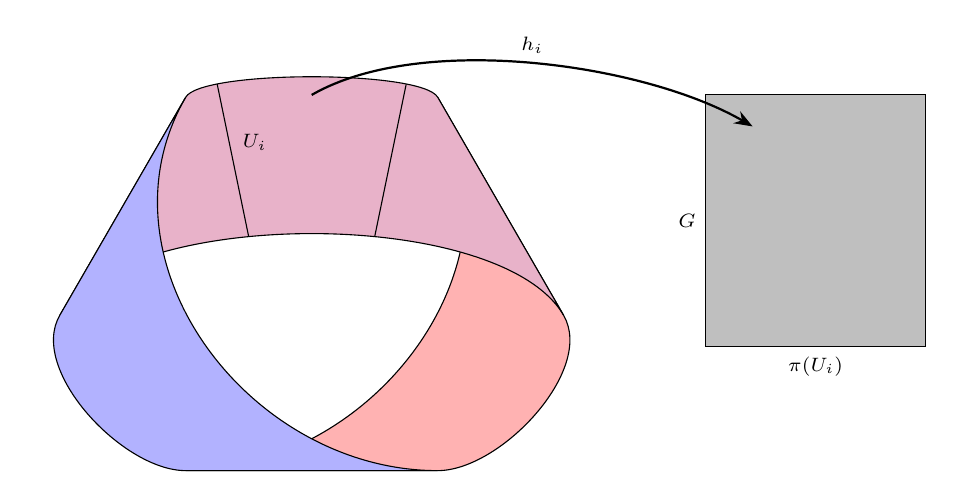
\begin{tikzpicture}[scale=0.8]
	%\draw[opacity=0.1] (-4.5,-4.5) grid (12.5,4.5);
	
	
%%%%     MOBIUS     %%%%

	%main points
	\coordinate (s1-) at ($(90+0-30:4) + (0,-1)$);
	\coordinate (s1+) at ($(90+0+30:4) + (0,-1)$);
	
	\coordinate (s2+) at ($(90+120-30:4) + (0,-1)$);
	\coordinate (s2-) at ($(90-120+30:4) + (0,-1)$);
	
	\coordinate (s3+) at (90+120+30:4);
	\coordinate (s3-) at (90-120-30:4);
	
	%\draw (s1-) -- (s2+) -- (s3-) -- (s1-);
	%\draw (s1+) -- (s3+) -- (s2-) -- (s1+);
	%\draw (s3+) -- (s3-);
	\colorlet{tmpb}{blue!30!};
	\colorlet{tmpr}{red!30!};
	\colorlet{tmpv}{blue!30!red!30!};
	\definecolor{tmpg}{gray}{0.75};
	
	
	% bande droite
	\draw[fill=tmpr] (s1-) .. controls  ($(s1-)+(-60:3)$) and  ($(s3+)+(0:3)$) .. 
		(s3+) -- (s3-) 
		.. controls ($(s3-)+(0:1)$) and ($(s2-)+(-60:1)$) .. 
		(s2-) -- cycle;
		
	% bande haut
	\draw[fill=tmpv] (s1-) .. controls  ($(s1-)+(120:0.5)$) and  ($(s1+)+(60:0.5)$) .. 
		(s1+) -- (s2+) 
		.. controls ($(s2+)+(60:2)$) and ($(s2-)+(120:2)$) .. 
		(s2-) -- cycle;
		
	% bande gauche
	\draw[fill=tmpb] (s1+) .. controls  ($(s1+)+(-120:3)$) and  	($(s3-)+(-180:3)$) .. 
		(s3-) -- (s3+) 
		.. controls ($(s3+)+(-180:1)$) and ($(s2+)+(-120:1)$) .. 
		(s2+) -- cycle;
		
		
	%%%%     CARTE LOCALE     %%%%
	
	% ouvert U_i
	\draw (-1,0.25) -- (-1.5,2.67) node[midway, above right]{$U_i$};
	\draw (1,0.25) -- (1.5,2.67);
	
	% carte
	\draw[fill=tmpg, shift={(6.25,-1.5)}] (0,0) -- (0, 4) node[midway, left]{$G$} -- (3.5,4) -- (3.5,0) -- cycle node[midway, below]{$\pi(U_i)$};
	
	% fleche vers la carte
	\draw[-Stealth, thick] (0,2.5) ..
	controls ($(0,2.5) + (30:2)$)  and ($(7, 2) + (180-30:2)$) .. (7, 2) node[midway, above]{$h_i$};
	
\end{tikzpicture}
	\includegraphics[width=0.55\textwidth]{fig/placeholder}
	\caption[Ruban de Mobius comme variété fibrée]{\DONE Représentation du ruban de Modius en tant que fibré. Les notations sont reprises de la \cref{def:VFP}.}
	\label{fig:ruban2modius}
\end{figure}
\skipl

Il existe toutes sortes de variétés fibrées dès lors qu'elles sont munies de structure remarquable. Celles qui vont nous intéresser sont dites principales\footnote{\itshape
	Bien que ce ne sera pas précisé, il sera toujours sous-entendu que les différentes variétés et cartes doivent avoir les mêmes niveaux de régularités pour que le tout reste cohérent.} :
\\
\begin{definition}[Variété fibrée principale] \label{def:VFP}
	Une \emph{variété fibrée principale} (VFP), ou \emph{fibré principal} est constituée de deux variétés différentielles $P$ et $B$ telles que :
	\begin{itemize}
		\item Il existe un groupe de Lie $G$ opérant à droite (ou à gauche) sur $P$ via l'application différentiable :
		\begin{equation} \label{eq:VFP_action}
			R\ :\ \begin{aligned}P\times G\ &\lr\quad\ \ P \\ (p,g)\ \ &\lmt\ R_g(p)\defeq p\cdot g = pg
			\end{aligned}
		\end{equation}
		
		\item Il existe une surjection différentiable $\ \pi:P\lr B\ $ telle que :
		\begin{equation} \label{eq:VFP_fibres}
			\forall p\in P,\quad \pi^{-1}\big(\pi(p)\big)=pG
		\end{equation}
		
		\item $P$ est munie d'un ensemble de paires $(U_i, h_i)$ tel que les $U_i$ forment un recouvrement de $B$ et tel que les $h_i : G\times U_i\lr \pi^{-1}(U_i)\subset P$ soient des difféomorphismes vérifiant :
		\begin{align*} \label{eq:VFP_atlas}
			\forall a,b\in G,\ \forall x\in B,\qquad h_i(ab,x) = h_i(a,x) \cdot b\qquad \text{et} \qquad \pi\circ h_i(a,x) = x
		\end{align*}
	\end{itemize}
	
	\begin{adjustbox}{valign=C,raise=1cm, minipage={1.1\linewidth}}
		\begin{wrapfigure}{r}{0.35\textwidth}
			\begin{tikzcd}[column sep=large]
				G\times U_i \arrow[d, "\pr{2}" left]  \arrow[r, "h" above]  & \pi^{-1}(U_i) \subset P \arrow[ld, "\pi" below right] \\
				U_i
			\end{tikzcd}
			%\caption{Digramme sûrement osef des jeux de projections entre $P$ et les cartes locales}
			\label{diagram_commu_VFP}
		\end{wrapfigure} 
		\vspace*{-0.5cm} % This is a fudge to align the top of the theorem environment with the image
		\skipl\par 
		La variété $B$ est appelée la \emph{base} de la VFP, $G$ son \emph{groupe structural} et $pG$ la \emph{fibre de $P$ passant par} $p$ et \emph{au dessus de} $\pi(p)\in B$. Le tout est notée $P(R, G, \pi, B)$ ou plus simplement $P(G,B)$.
		
		Les fibres $pG$ sont toutes difféomorphes à $G$ et $B$ est difféomorphe à $P/G$. Le diagramme commutatif ci-contre résume la situation ($\text{pr}_i$ est la projection canonique sur la $i-$ème composante).
	\end{adjustbox}
\end{definition}
\skipl 


L'ensemble $\big\{(U_i\times G, {h_i}^{-1})\big\}_i$ est l'équivalent d'un atlas pour les variétés différentielles classiques mais adapter pour tenir compte de la structure fibré de $P$ et de l'action de $G$. Expliciter les changements de cartes dans $P$, ce fait comme suit.
\\
D'abord, $P$ étant localement difféomorphe à un produit $G\times U_i$, on peut y tracer des graphes appelés \emph{sections locales}, comme sur les \Cref{fig:section_local,fig:section_cano} ci-dessous. Formellement, une section locale au dessus  de $U_i \subset B$ est une application $\sigma : U_i \lr P$ vérifiant :
\[\pi\circ \sigma = id_{{\displaystyle |}U_i}\]
\begin{figure}[H]
	\begin{floatrow}
		\ffigbox{\caption[Représentation d'une section local]
			{\DONE Représentation d'une section local $\sigma$ au dessus de $U_i\subset B$ de dimension 2. Comme $P$ n'est pas un produit à proprement parler, $\sigma$ est représenté dans $G\times U_i$ à travers $h_i$.}
			\label{fig:section_local}}{
			\includegraphics[width=0.45\textwidth]{fig/placeholder}
			%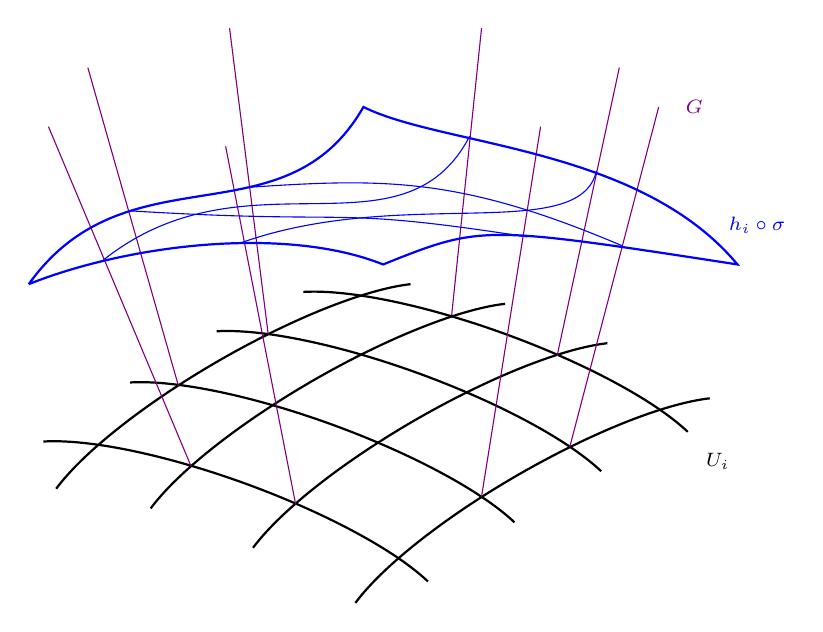
\begin{tikzpicture}%[scale=0.9]
	%\draw[opacity=0.1] (-4.5,-4.5) grid (4.5,4.5);

	%\draw (-1,-4)  .. controls (0,-2.5) and (1.5,-1.75) ..  (4,-2);

% BASE

	% gauche
	\draw[thick, xshift=1.3cm, yshift=-3.2cm, rotate=30]
		(3,0) arc [start angle=30, end angle =150, radius = 3, y radius = 0.75];
		
	\draw[thick, xshift=0cm, yshift=-2.5cm, rotate=30]
		(3,0) arc [start angle=30, end angle =150, radius = 3, y radius = 0.75];
		
	\draw[thick, xshift=-1.3cm, yshift=-2cm, rotate=30]
		(3,0) arc [start angle=30, end angle =150, radius = 3, y radius = 0.75];
		
	\draw[thick, xshift=-2.5cm, yshift=-1.75cm, rotate=30]
		(3,0) arc [start angle=30, end angle =150, radius = 3, y radius = 0.75];
		
	% droite
	\draw[thick, xshift=-2.5cm, yshift=-3cm, rotate=-20]
		(3,0) arc [start angle=30, end angle =150, radius = 3, y radius = 0.75];
	
	\draw[thick, xshift=-1.4cm, yshift=-2.25cm, rotate=-20]
		(3,0) arc [start angle=30, end angle =150, radius = 3, y radius = 0.75];
	
	\draw[thick, xshift=-0.3cm, yshift=-1.6cm, rotate=-20]
		(3,0) arc [start angle=30, end angle =150, radius = 3, y radius = 0.75];
	
	\draw[thick, xshift=0.8cm, yshift=-1.1cm, rotate=-20]
		(3,0) arc [start angle=30, end angle =150, radius = 3, y radius = 0.75];
	
	
% FIBRES

	\draw[violet] (-1.36,-3.05) -- (-2.25,1.5);
	\draw[violet] (1,-2.95) -- (1.75,1.75);
	
	\draw[violet] (-2.69,-2.56) -- (-4.5,1.75);
	\draw[violet] (2.12,-2.32) -- (3.25,2);
	
	\draw[violet] (-2.85,-1.54) -- (-4,2.5);
	\draw[violet] (1.96,-1.16) -- (2.75,2.5);
	
	\draw[violet] (-1.71,-0.88) -- (-2.2,3);
	\draw[violet] (0.62,-0.65) -- (1,3);
	
	
% SECTION

	%frame
	\draw[thick, blue] (-4.75,-0.25) .. controls (-3.5,1.5) and (-1.5,0.25) ..  
		(-0.5,2) .. controls (0.5,1.5) and (3,1.5) ..
		(4.25,0) .. controls (1,0.5) ..
		(-0.25,0) .. controls (-1.5,0.5) and (-3.5,0.25) ..
		(-4.75,-0.25);
		
	% coordo droite
	\draw[blue] (-3.45,0.68) .. controls (-0.5,0.5) and (-1,0.75) .. (1.58,0.35);
	\draw[blue] (-1.95,0.98) .. controls (-0.2,1.1) and (0.75,1.1) .. (2.78,0.24);
	
	%coordo gauche
	\draw[blue] (-3.81,0.05) .. controls (-2,1.5) and (0,0) .. (0.85,1.63);
	\draw[blue] (-2.04,0.28) .. controls (0,1) and (2.25,0.25) .. (2.46,1.19);
	
% NOTATION
	\draw (4,-2.5) node{ $U_i$};
	\draw (3.7,2) node{\color{violet} $G$};
	\draw (4.5,0.5) node{\color{blue} $h_i \circ \sigma$};
	
\end{tikzpicture}
			}
		
		\ffigbox{ \caption[Représentation de la section canonique]
			{Représentation de la section canonique définie par rapport à $G$ avec une seconde section  $\sigma(x) = \sigma_i(x)\cdot g(x)$. Cette fois $B$ est une variété de dimension 1. % Sont également représentés leur espaces tangents horizontaux respectifs avec la transformation permettant de passer l'un à l'autre.
			}
			\label{fig:section_cano}}{
			\includegraphics[width=0.45\textwidth]{fig/placeholder}}
	\end{floatrow}
\end{figure}
\noindent
Ensuite, les hypothèses sur $P(G,B)$ sont telles que $G$ agit transitivement et librement (ou sans point fixe) sur $P$. C'est-à-dire que, sur une même fibre, tout point peut être atteint par n'importe quel autre via l'action de $G$ (transitivité) :
\begin{align*}
	\forall x\in B,\quad \forall p,q\in P_x,\ \exists t(p,q)\in G\ |\ p = q\cdot t(p,q) 
\end{align*}
et que la seule façon de laisser les points invariants par cette même action est de passer par l'élément neutre $e$ (libre) :
\begin{align*}
	\forall (p,g)\in P\times G,\quad p = p\cdot g\ \Lr\ g=e
\end{align*}
\\
De la transitivité de $G$, découle le fait que toutes les sections locales $\sigma$ au dessus de $U_i$ peuvent s'écrire à partir d'une même section $\sigma_i$ via la formule :
\[\forall x\in B,\qquad \sigma(x) = \sigma_i(x) \cdot t\big(\sigma_i(x), \sigma(x)\big)\]
Son caractère libre, lui assure l'unicité d'un choix canonique de section $\sigma_i$ sur $U_i$. Elle est donnée par :
\[{h_i}(x,e) = \sigma_i(x)\]
Cela mène à la définition :
\begin{definition}[Fonctions de transitions]
	L'intersection de deux cartes est noté $U_{ij} = U_i\cap U_j$ et le passage d'une section locale canonique est donné par :
	\[\forall x\in U_{ij},\qquad \sigma_j(x) = \sigma_i(x) \cdot t\big(\sigma_i(x), \sigma_j(x)\big)\]
	L'élément de $G$, $t(\sigma_i, \sigma_j)$, est alors appelé \emph{fonction de transition} et sera noté $\varphi_{ij}$. Elle fait effectivement la transition entre deux cartes dans le sens où :
	\[\forall (g,x)\in G\times U_{ij},\qquad {h_i}^{-1} \circ h_j(g,x) = \big( \varphi_{ij}(x)g, x \big)\]
\end{definition}
\skipl




\subsubsection{Le fibré $\bf{\VFP}$}\label{subsec:SUPC_VFP}

Dans notre cas c'est $\S{n}$ qui fait office d'espace totale avec pour base $\PC{n}$ et de groupe structural $\U{1}$.
\\
Pour obtenir la projection de $\S{n}$ sur $\PC{n}$, il suffit de prendre la restriction de $\pi$ à $\S{n}$. En tenant compte de la normalisation, les coordonnées locales sur $\PC{n}$ se réécrivent, $\forall w\in U_i$ :
\begin{align*}
	w^\mu = \frac{z^\mu}{z^i} &= \frac{z^\mu}{|z^i|e^{i\arg (z^i)}} = \frac{z^{\mu}}{\sqrt{1 - \sum_{\nu \neq i} |z^\nu|^2}} e^{-i\arg(z^i)}  &  \text{car }\quad \sum \big|z^\nu\big|^2 = \|z\|^2 = 1
\end{align*}
\\
On constate bien que $w^\mu$ n'est défini par rapport à $z^\mu$ qu'à un choix de phase $e^{-i\arg z^i}\in \U{1}$ près. À l'inverse, un représentant $z_i$ dans $\S{n}$ de $w\in U_i$ aura pour coefficient :
\begin{align*}
	\forall \mu\neq i,\quad {z_i}^\mu &= \frac{w^\mu}{\|w\|}e^{i\theta}  &  {z_i}^i &= \frac{1}{\|w\|}e^{i\theta} 
\end{align*}
\\
La norme de $w$ étant à comprendre au sens des coordonnées locales sur $U_i$\footnote{\itshape
	C'est un abus de notation, $w$ n'a pas de norme en ce sens là puisqu'elle dépend du choix de carte $U_i$. Mais ici tout le raisonnement est purement local, donc ce n'est pas un problème.
} :
\begin{align*}
	\|w\|^2 = \big\|(w^\mu)_{1\leq \mu\leq n}\big\|^2 = \frac{1}{|{z_i}^i|^2}\sum_{\nu \neq i} \big|{z_i}^\nu\big|^2 = \frac{1 - |{z_i}^i|^2}{|{z_i}^i|^2} &\Llr\ \big| {z_i}^i \big|^2 \|w\|^2 = 1 - \big|{z_i}^i\big|^2 \\
	&\Llr\ \big|{z_i}^i\big|^2 = \frac{1}{1 + \|w\|^2} \\
	&\Llr\ \big|{z_i}^i\big| = \frac{1}{\sqrt{1 + w^\nu \congu{w}_\nu}}
\end{align*}
D'où l'expression des coefficients de $z_i\in\S{n}$ :
\begin{align*}
	 \forall \mu\neq i,\quad {z_i}^\mu &= \frac{w^\mu}{\sqrt{1 + w^\nu \congu{w}_\nu}}e^{i\theta}  &  {z_i}^i &= \frac{1}{\sqrt{1 + w^\nu \congu{w}_\nu}}e^{i\theta} 
\end{align*}
\\

Tout cela permet d'écrire $\S{n}$ comme une variété fibrée principale :
\begin{proposition}
	La $(2n+1)-$sphère $\S{n}$, vue comme variété plongée dans $\C^n$ est une VFP de base $\PC{n}$ et de fibre type $\U{1}$. L'action de $\U{1}$ sur $\S{n}$ est induite par la multiplication par un scalaire complexe et où :
	\begin{itemize}
		\item La fibration $\pi$ est la projection canonique de $\S{n}$ sur $\PC{n}$ :
		\begin{equation}
			\pi\ :\ \begin{aligned} \S{n}\ &\lr\ \PC{n} \\ z\quad\ &\lmt\ \ [z]\end{aligned}
		\end{equation}
		
		\item Les cartes locales $h_i$ s'écrivent :
		\begin{equation}
			\forall w \in U_i,\ \forall e^{i\theta}\in\U{1},\  h_i(w,e^{i\theta}) = \frac{(w^0,\cdots, 1,\cdots, w^n)}{\sqrt{1 + w^\nu \congu{w}_\nu}}e^{i\theta} \in \S{n}
		\end{equation}
		
		\item Les sections canoniques $\sigma_i$ au dessus des $U_i$, elles,  sont définies par :
		\begin{equation}
			\forall w \in U_i,\ \sigma_i(w) = h_i(w, 1) = \frac{1}{\sqrt{1 + w^\nu \congu{w}_\nu}}(w^0,\cdots, 1,\cdots, w^n)
		\end{equation}
		
		\item Les fonctions de transitions entre deux cartes $U_i$ et $U_j$ s'écrivent :
		\begin{align}
			\varphi_{ij}(w) &= e^{-i \arg (z_i^i)} e^{i \arg (z_j^j)}  &  \text{ où }&\qquad z_{i,j} = \phi_{i,j}(w)
		\end{align}
	\end{itemize}
\end{proposition}
\skipl




\subsection{Connexion et relèvements horizontaux}\label{subsec:connexion2VFP}

Le cadre étant posé, pour retrouver la notion de fréquence instantanée, il est nécessaire de munir $\VFP$ d'une connexion. Cette dernière est introduite comme suit.

\subsubsection{Définition générale}\label{subsec:def2conn}

Comme $P$ ressemble localement à un produit $G\times U_i$, il est utile de séparer ses espaces tangents $\tg[p]{P}$ comme une somme directe d'espaces tangents respectivement aux fibres et à la base. Conformément aux représentations précédentes (\cref{fig:ruban2modius,fig:section_cano,fig:section_local}), les premiers sont appelées espaces tangents \emph{verticaux}, les seconds \emph{horizontaux} et l'on note :
\[\forall p\in P,\qquad \tg[p]{P} = \vg[p]{P} \oplus \hg[p]{P}\]
\\
Les tangents verticaux $\vg[p]{P}$ se définissent canoniquement via $\pi$, en tant que noyau de sa différentielle :
\[\vg[p]{P} \defeq \Ker (\tg[p]{\pi}) = \big\{ v\in\tg[p]{P}\ |\ \tg[p]{\pi}(v)=0 \big\}\]
\\ 
Ce n'est en revanche pas le cas des espaces horizontaux. Il faut donc faire un choix pour les $\hg[p]{P}$ et c'est ce choix qui est appelé \emph{connexion} (elle connecte les espaces tangents entre eux).
Comme pour les verticaux, ces sous-espaces peuvent être caractérisés par une 1-forme différentiable $\conn$ sur $P$ à valeur dans $\vg{P}$, auquel cas :
\[\forall p\in P,\quad \hg[p]{P} = \Ker(\conn_p)\]
\skipl

Dans le cas des VFP, une connexion doit en plus avoir de bonnes propriétés au regard de l'action de $G$ sur $P$, aboutissant à la définition :

\begin{definition}[Connexion sur VFP] \label{def:connexion2VFP}
	Une \emph{connexion} sur une VFP $P(G,B)$ est la donnée d'un sous-espace tangent, $\hg[p]{P}\subset \tg[p]{P}$, en tout point de $p\in P$ tel que :
	\begin{itemize}
		
		\item $\hg{P}$ dépend différentiellement de $p$ (``dépendre différentiellement'' à un sens précis pour les sous-espaces mais qui ne sera pas utile pour la suite).
		
		\item $\hg[p]{P}$ est supplémentaire à $\vg[p]{P}$ dans $\tg[p]{P}$ :
		\begin{equation}\label{eq:TP=V+H}
			\tg[p]{P} = \vg[p]{P} \oplus \hg[p]{P}
		\end{equation}
		
		\item l'assignation des $\hg[p]{P}$ est invariante par l'action de $G$ au sens où :
		\begin{equation}\label{eq:conn_G-inv}
			\forall (p,g)\in P\times G,\quad \hg[R_g(p)]{P} = R_{g*} (\hg[p]{P}) = \big\{R_{g*}(\bf{v})\ |\ \bf{v} \in \hg[p]{P} \big\}
		\end{equation}
		Que l'on notera plus simplement :
		\begin{equation}
		\forall (p,g)\in P\times G,\quad \hg[p\cdot g]{P} = \hg[p]{P}\cdot g = \big\{\bf{v}\cdot g\ |\ \bf{v} \in \hg[p]{P} \big\}
		\end{equation}
	\end{itemize}
\end{definition}
\skipl

Au delà d'assurer une compatibilité entre $H$ et $G$, l'équation \eqref{eq:conn_G-inv} permet de n'avoir à définir la connexion qu'en un seul point de chaque fibre, les autres se déduisant par cette formule. 
Concrètement, pour tout point de la base $x\in U_i$, il suffit de la définir en $\sigma_i(x) = h_i(e, x)$, de sorte que l'espace horizontal en tout autre point $\ p=h_i(g, x) = \sigma_i(x)\cdot g$ au dessus de $x$ sera donné par :
\[\hg[p]{P} = \hg[\sigma_i(x)]{P}\cdot g\]
\\
Aussi, le fait que $G$ soit un groupe de Lie permet de lier son algèbre $\mathfrak{g}\cong \tg[e]{G}$ aux tangents verticaux via l'application $\#$ : \footnote{\itshape 
	Les vecteurs tangents étant des formes linéaires, $A^\#(p)$ est plus précisément définie par l'application :
	\[A^\#(p) : f\ \lmt\  \frac{d}{dt} f\big( p\cdot \exp(tA) \big)\Big|_{t=0}\]}
\begin{equation} \label{eq:alg2vg}
	\forall (p,A)\in P\times \mathfrak{g},\ \forall f\in\conti{P}{\R},\quad A^\#(p) = \frac{d}{dt} p\cdot \exp(tA) \Big|_{t=0}\in\vg[p]{P}
\end{equation}
\\
Sachant cela, toujours dans le cas des VFP, la $1-$forme de connexion est à valeur dans $\mathfrak{g}$ :

\begin{definition}[$1-$forme de connexion] \label{def:1-form2conn}
	La \emph{$1-$forme de connexion} $\conn$ d'une VFP $P(G,B)$ est définie comme la 1-forme différentiable sur $P$ à valeur dans $\mathfrak{g}$ (\ie~en tout point $p\in P$, $\conn_p$ est à valeur de $\tg[p]{P}$ dans $\mathfrak{g}$), telle que $\forall p\in P$ :
	\begin{align} \label{eq:1-form2conn}
		\forall A\in \mathfrak{g},\ \conn_p\big(A^\#(p)\big) &= A  &  \hg[p]{P} &= \Ker(\conn_p)
	\end{align}
	\begin{equation} \label{eq:1-form_G-inv}
		\forall \bf{v}\in\tg[p]{P},\quad \conn_{p\cdot g}(\bf{v}\cdot g) \defeq \conn_{p\cdot g}(R_{g\, *}(\bf{v})) = g^{-1}\conn_p(\bf{v})g
	\end{equation}
	\skipl
	
	Tout comme les $H[p]{P}$, la troisième égalité assure que $\conn$ n'a besoin d'être définie que sur un point de chaque fibre. Cela permet de définir $\conn$ localement non pas sur $\ U_i\times G$, mais seulement sur $\ U_i \cong U_i \times \{e\}$. Ainsi, $\conn$ induit une 1-forme sur les cartes $U_i$ par l'image réciproque des sections canoniques $\sigma_i$. Elles sont notées $\locconn_i \defeq \sigma_i^*\conn$ et sur le chevauchement $U_i\cap U_j$, elles vérifient :
	\begin{equation}\label{eq:conn_local}
		\locconn_j = {\varphi_{ij}}^{-1} \locconn_i \varphi_{ij} + {\varphi_{ij}}^{-1} d \varphi_{ij}
	\end{equation}
\end{definition}
\skipl


Munir $P(G,B)$ d'une connexion permet, entre autre de définir la notion de relèvement horizontal :
\begin{definition}[Relèvement horizontal]
	Étant donné une trajectoire $\ \rho : \R\ \lr B\ $ sur la base et un point $\gamma_0\in \rho(0)G$ au dessus de $\rho(0)$, il existe un unique relèvement $\gamma$ de $\rho$ dont les vecteurs tangents sont tous horizontaux. \ie~tel que $\forall t\in\R$ :
	\begin{align} \label{eq:condi2hori_lift}
	\pi\circ\gamma(t) &= \rho(t)  &  \dot{\gamma}(t) &\in \hg[\gamma(t)]{P} &  \gamma(0) &= \gamma_0
	\end{align}
	\\
	On parle de \emph{relèvement horizontal} (\emph{horizontal lift}, ou \emph{transport parallèle} de $\gamma_0$ le long de $\rho$) puisque $\gamma$ n'a pas de déplacement vertical au sens de la connexion. Du point de vue de la 1-forme $\omega$, si $\gamma$ s'écrit localement $\gamma_i = \sigma_i(\rho) g_i$, alors $g_i$ vérifie l'équation (d'où vient l'unicité du relèvement) :
	\begin{equation} \label{eq:EDP2hori_lift}
		\frac{d}{dt}g_i(t)  = - \locconn_i\rho(t) \cdot g_i(t)
	\end{equation}
	\\
	Si maintenant $\gamma$ est une trajectoire de $P$, on dira, par abus de langage, que $\Tilde{\gamma}$ est le relèvement horizontal de $\gamma$ si c'est le relèvement horizontal de sa projection $\pi\circ\gamma$ avec la condition initiale $\ \Tilde{\gamma}(0) = \gamma(0)$.
\end{definition}
\skipl

Pour la suite, il sera utile d'avoir l'expression d'une trajectoire $\gamma:\R\lr P$ par rapport à son relèvement horizontale $\Tilde{\gamma}$. Pour l'obtenir, on note  $\gamma = \Tilde{\gamma}\cdot g$, de sorte que sa dérivée s'écrive :
\[\dot{\gamma} = \dot{\Tilde{\gamma}}\cdot g + \Tilde{\gamma}\cdot dg = \dot{\Tilde{\gamma}}\cdot g + \gamma \cdot g^{-1}dg\]
\\
Ce à quoi on applique $\conn$, donnant :
\begin{align*}
	\conn_\gamma(\dot{\gamma}) &= \conn_\gamma\big( \dot{\Tilde{\gamma}}\cdot g \big) + \conn_\gamma \big( \gamma \cdot g^{-1}dg \big) \\
	&= g^{-1}\conn_{\Tilde{\gamma}}\big(\dot{\Tilde{\gamma}} \big) g + \conn_\gamma \big( \gamma \cdot g^{-1}dg \big)   &  &\text{d'après \eqref{eq:1-form_G-inv}} \\
	&= \conn_\gamma \big( \gamma \cdot g^{-1}dg \big)  &  &\text{car $\Tilde{\gamma}$ est horizontale}
\end{align*}
\\
Le terme $g^{-1}dg$ restant étant un vecteur de $\ g^{-1}\tg[g]{G}\cong \tg[e]{G}\cong \mathfrak{g}$ et :
\[\conn_\gamma(\dot{\gamma}) = \conn_\gamma \big( \gamma \cdot g^{-1}dg \big) = \conn_\gamma \big( (g^{-1}dg)^\#(p) \big) = g^{-1}dg\]
\\
D'où $\ \gamma = \Tilde{\gamma}\cdot g\ $ avec $g$ est solution de :
\begin{equation} \label{eq:deviation2hozi}
	\frac{d}{dt}g(t)  = g(t) \conn_{\gamma(t)}\big( \dot{\gamma}(t) \big)
\end{equation}
\skipl



\subsubsection{Choix de connexion sur $\bf{\VFP}$}\label{subsec:conn2SUPC}

Dans le cas de  $\VFP$, la métrique sur $\S{n}$ induit naturellement un choix de connexion car la projection $\pi$ est une submersion dite riemannienne \cite{kayban_riemannian_nodate}. Formellement, c'est dire que la projection de $\S{n}$ sur $\PC{n}$ est telle que :
\begin{equation} \label{eq:sub_riem}
	\forall p\in \pi^{-1}(w),\ \forall \bf{u},\bf{v}\in\tg[p]{\S{n}},\quad  g_{\pi(p)}\big( \pi_*\bf{u}, \pi_*\bf{v}\big) = \langle \bf{u}_H, \bf{v}_H\rangle
\end{equation}
\\
où $g$ est la partie réelle\footnote{\itshape
	Cette métrique induite ne peut pas être hermitienne car $\S{n}$ n'est pas une variété complexe.}
hermitienne de la métrique de Fubini-Study. Plus concrètement, les espaces tangents de $\S{n}$ s'écrivent :
\[\tg[p]{\S{n}} = \Vec\{p\}^\perp \defeq \big\{ \bf{v}\in\C^{n+1}\ |\  \Re e \langle \bf{v},p\rangle = 0\big\}\]
\\
et sachant que $ip\in \Vec\{p\}^\perp$, ils se séparent en deux composantes orthogonales :
\[\tg[p]{\S{n}} = \Vec\{p\}^\perp = \Vec\{ip\} \oplus \Vec\{ip\}^\perp\]
\\
Ainsi, la nature de $\pi$ \eqref{eq:sub_riem} est telle que le premier membre est l’espace tangent vertical à $p$ et le second invariant par l'action de $\U{1}$ :
\[\forall e^{i\theta}\in\U{1},\quad \Vec\big\{i(e^{i\theta}p)\big\}^\perp = \Vec\{ip\}^\perp\]
\\
Ce qui permet de poser $\ \hg[p]{\S{n}} \defeq \Vec\{ip\}^\perp\ $ et donne directement la 1-forme associée :
\[\begin{aligned}
	\hg[p]{\S{n}} &= \big\{\bf{v}\in\tg[p]{\S{n}}\ |\ \Re e \langle \bf{v}, ip \rangle = 0\} \\
	&= \big\{\bf{v}\in\tg[p]{\S{n}}\ |\ \Im m\langle \bf{v}, p \rangle = 0\}
\end{aligned}
\quad \Llr\quad \conn_p(\bf{v}) = \Im m\langle \bf{v},p\rangle\]
\\
Enfin, comme l'algèbre de Lie de $\U{1}$ est $\u{1}\cong i\R$, il convient de de poser :
\begin{equation}\label{eq:conn2sub_riem}
	\forall p\in\S{n},\ \forall \bf{v}\in\tg[p]{\S{n}},\qquad \conn_p(\bf{v}) \defeq i\Im m\langle \bf{v},p\rangle
\end{equation}
\\
Un tel choix de connexion n'est pas anodin d'un point de vue signal puisque $\conn$ donne la fréquence instantanée telle que définie dans la \cref{part:param_instant} précédente et c'est la première chose qui sera justifié dans la partie suivante.
\\




\section{\wip Interprétation des phases sur $\bf{\VFP}$} \label{sec:phases_dans_VFP}

Résumons la situation. Pour étudier le comportement fréquentiel d'un signal multivarié complexe, il est utile de voir l'espace de tel signaux, $\C^{n+1}$, comme le produit :
\[\C^{n+1} \cong \R^{+_*} \times \S{n} \overset{\text{-ish}}{\cong} \R^{+_*} \times \U{1} \times \PC{n}\]
Cette égalité n'étant valable que localement, l'établir proprement nécessite de passer par le formalisme des fibrés, qui plus et principaux.
\\
Dans ce cadre, la VFP $\VFP$ est naturellement -- par sa métrique -- munie d'une connexion qui, par ailleurs, n'est pas sans rappeler à la formule de la fréquence instantanée \eqref{eq:phas_inst_v1} vue en première partie.
\\
Reste alors à clairement établir ce lien et comprendre comment émerge la phase géométrique dans ce contexte, chose qui sera fait dans cette partie.
\\



\subsection{Fréquence instantanée et phase dynamique}


Pour comprendre pourquoi le choix de connexion \eqref{eq:conn2sub_riem} est justifié du point de vue signal, on se propose de prendre le problème par l'autre bout : comment définir la notion de fréquence instantanée d'un signal dans le fibré $\VFP$ ?
\\
 
Comme, à chaque instant $t$, un signal $\gamma$ sur $\S{n}$ est représenté par une paire $(e^{i\alpha(t)}, \rho(t))\in\U{1}\times\PC{n}$ à travers les $h_i$,  l'un serait tenté de voir $\alpha(t)$ comme la fréquence du signal et $\rho(t)$ comme son état de polarisation.
\\
Le problème de cette représentation est qu'elle dépend du choix de carte $U_i$, ainsi sur l'intersection $U_{ij}$, $\gamma$ aurait (au moins) deux notions de fréquence instantanée.
\\

C'est là qu'intervient la connexion. D'une part, la 1-forme $\conn$ associée est définie globalement sur le fibré, autrement dit, elle est indépendante des représentations locales de $\gamma$.
\\
D'autre part, le relèvement horizontal $\Tilde{\gamma}$ d'une courbe $\rho\subset\PC{n}$, par définition, n'a pas de variation verticale. Dans notre contexte, cela signifie que $\Tilde{\gamma}$ n'a pas de variation dans la direction de $\U{1}$, donc son état de polarisation (composante sur $\PC{n}$) varie mais pas ses ``fréquences''.
\\
Ainsi, le relèvement horizontale $\Tilde{\gamma}$ d'un signal $\gamma$ s'interprète comme une version de ce dernier dénuée de toute fréquence instantanée.
L'action $\alpha$ permettant de passer de $\Tilde{\gamma}(t)$ à $\gamma(t)$ (\ie~$(t) = e^{i\alpha(t)} \Tilde{\gamma}(t)$) peut alors être comprise comme l'ajout d'une fréquence instantanée (voir \cref{fig:freq_inst_geodiff,fig:horiz_lift_2var} ci-dessous)	
\\

\begin{remarque}
	Un signal qui n'aurait pas de fréquence instantanée mais une polarisation instantanée n'a pas vraiment de sens. 
	Cela renvoi à notre discussion de première partie : la fréquence instantanée d'un signal univarié devait contenir les hautes fréquences et son amplitude les basses.
	Ici le problème est le même, mais avec l'état de polarisation en lieu de l’amplitude. Pour s'en convaincre, il est utile de retourner sur le cas bivarié.
	\\
	La projection sur $\PC{2}$ de $\gamma$ représente l'ellipse de polarisation instantanée. 
	Mais si $\gamma$ n'as pas de fréquence instantanée, alors $\gamma(t)$ n'est plus représenté que par le sommet de l’ellipse paramétrée par $\rho_\gamma$. 
	L'on pourrait alors argumenter que tout signal peut être décrit par la seule variation de son état de polarisation, ce qui est parfaitement inintéressant.
	
	Cette vision du relèvement horizontal est donc purement formelle et, si elle à bien un sens géométrique, elle ne correspond du point de vue du signal.
\end{remarque}
\skipl

\begin{figure}[h]
	\begin{floatrow}		
		\ffigbox{ \caption[Interprétation géométrique de la fréquence instantanée]
			{Fréquence instantanée d'un signal $x$ vu comme variation vertical de $x$ par rapport à son relèvement horizontale $\Tilde{x}$ associé. À noter que $\Tilde{x}$ ne dépend pas des cartes mais dépend de la trajectoir $\rho_x$ de $x$ sur $\PC{n}$.}
			\label{fig:freq_inst_geodiff}}
			{\includegraphics[width=0.45\textwidth]{fig/placeholder}}
			
		\ffigbox{ \caption[Exemple relèvement horizontale]
			{Exemple du relèvement horizontale d'une signal bivarié}
			\label{fig:horiz_lift_2var}}
		{\includegraphics[width=0.45\textwidth]{fig/placeholder}}
	\end{floatrow}
\end{figure}

En admettant l'interprétation de la 1-forme de connexion comme fréquence instantanée, les discussions de première partie (\Cref{subsec:intro_phased}) suggèrent de choisir là encore :
\begin{equation} \label{eq:conn2SUPC}
	\forall p\in\S{n},\ \forall \bf{v}\in\tg[x]{\S{n}},\quad \conn_p(\bf{v}) = i\Im m \langle \bf{v}, p\rangle
\end{equation}
\\
La phase dynamique, s'interprète alors comme la déviation du signal par rapport à son relèvement horizontal. Ainsi, $\ g = e^{i\phased(\gamma)}\ $ est solution de \eqref{eq:deviation2hozi}, qui se réécrit alors :
\[\forall t\in\R,\quad \left\{ \begin{aligned}
	g'(t)  &= g(t)\, i\Im m \big\langle \dot{\gamma}(t) , \gamma(t) \big\rangle \\
	g(t_0) &= 1
\end{aligned}\ \right. \Llr\ g(t) = e^{i \int_{t_0}^t \Im m\langle \dot{\gamma}(s) , \gamma(s) \rangle ds}\]
\\
Ce qui redonne la formule :
\begin{equation}\label{eq:phased_vgeodiff}
	\phased(\gamma, t_0, t) = \int_{t_0}^t \Im m\big\langle \dot{\gamma}(s) , \gamma(s) \big\rangle ds
\end{equation}
\skipl

Chose importante tout de même : si cette définition de la phase dynamique est bien indépendante du choix de carte, elle dépend en revanche du relèvement horizontale de $\gamma$ et, \afortiori, de la trajectoire de la projection $\pi(\gamma)$ de $\gamma$ sur $\PC{n}$. C'est de là que va émerger la phase géométrique,.
\\



\subsection{Phase géométrique}

Notamment dans le cadre quantique, la phase géométrique est connue pour avoir deux interprétations géométriques \cite{bohm_geometric_2003, chruscinski_geometric_2004,faure_introduction_2022} : soit comme conséquence d'un transport parallèle sur $\S{n}$ soit comme une mesure de l'aire de la surface entourée par le signal projeté sur $\PC{n}$. Ces résultats sont redémontrés dans cette section (avec les détails en annexes) dans notre cadre -- plus général --- et réinterpréter en terme de signal.

Pour se faire, sera d'abord traité le cas particulier des signaux cycliques (\Cref{subsec:phase_g2cycl,subsec:phase_g2aire}) et il sera ensuite montré que, du cas général, il est toujours possible de s'y ramener (\Cref{subsec:phase_g2geode}).
\skipl



\subsubsection{... du point de vue de la connexion} \label{subsec:phase_g2cycl}

Dans toute la suite un signal $\gamma$ de $\S{n}$ sera dit \emph{cyclique} si entre les instants $t_0$ et $t$, $\gamma$ retourne dans la même fibre :
\begin{equation}\label{eq:def2cycl}
	\exists \alpha \in\R\ |\ \gamma(t) = e^{i\alpha}\gamma(t_0)
\end{equation}
\\
Dit autrement, la projection de $\gamma$, $\rho_\gamma \defeq \pi\circ\gamma$ forme un lacet sur $\PC{n}$.
Cette hypothèse est très restrictive puisqu'elle ne peut arriver que certain instant, sans quoi $\gamma$ n'aurait qu'un mouvement vertical, ce qui n'est d'autant plus contraignant.
\\

Cela étant dit, elle a le bon goût d'énormément simplifier les choses puisque, comme tout ce passe dans la même fibre, il est très simple calculer et d'annuler individuellement les phases de $\gamma$. 
\\
Suivant les travaux de Aharonov \& Anandan \cite{aharonov_phase_1987} et les explications de Bohm \cite{bohm_geometric_2003}, la première remarque est que, comme $\gamma(t_0)$ et $\gamma(t)$ sont dans une même fibre, la phase totale est donné par le paramètre $\alpha$ de \eqref{eq:def2cycl} :
\begin{equation}\label{eq:phase_t-cycl}
	e^{i\phaset} = e^{i\alpha} = t\big( \gamma(t_0), \gamma(t) \big)
\end{equation}
\\
La phase dynamique, conformément à ce qui a été dit plutôt, donne la déviation au relèvement horizontale $\Tilde{\gamma}$ :
\begin{equation}\label{eq:phase_d-cycl}
	e^{i\phased}= t\big( \Tilde{\gamma}(t), \gamma(t) \big)
\end{equation}
\\
La phase géométrique s'écrit alors :
\begin{equation}\label{eq:phase_g-cycl}
	\begin{aligned}
		e^{i\phaseg}= e^{i\phaset} e^{-i\phased} &= t\big( \gamma(t_0), \gamma(t) \big)\ t\big( \Tilde{\gamma}(t), \gamma(t) \big)^{-1} \\
		&= t\big( \gamma(t_0), \gamma(t) \big)\ t\big( \gamma(t), \Tilde{\gamma}(t) \big) \\
		&= t\big( \Tilde{\gamma}(t_0), \Tilde{\gamma}(t) \big)  &  
		&&  &&  &&  && \text{car }\gamma(t_0) &= \Tilde{\gamma}(t_0)
	\end{aligned}
\end{equation}
\\
Elle correspond donc au déplacement vertical dû à la trajectoire de $\Tilde{\gamma}$. Dit autrement, elle mesure la déviation du au transport parallèle le long de $\gamma$. Les trois dernières formules, \cref{eq:phase_t-cycl,,eq:phase_d-cycl,eq:phase_g-cycl}, sont représentées dans la \Cref{fig:phases-cycl} ci-dessous : 

\begin{figure}[h]
	\includegraphics[width=0.6\textwidth]{fig/placeholder}
	\caption[Représentation des trois phases de $\gamma$ dans le cas pseudo-cyclique]{Représentation des trois phases de $\gamma$ dans le cas pseudo-cyclique.}
	\label{fig:phases-cycl}
\end{figure}

\noindent Vu ainsi, il est clair que $\phaseg$ est complètement indépendante du relèvement $\gamma$ par rapport à $\rho_\gamma$, dit autrement, qu'elle est invariante par transformation de jauge. De même, elle ne dépend que de $\gamma(t_0)$ et $\Tilde{\gamma}(t)$, ce qui montre qu'elle est invariante par reparamétrisation de $\gamma$.
\\

Cette description de  $e^{i\phaseg}$ est plus connue sous le nom d’holonomie du lacet $\rho_\gamma$. De façon généralement, le groupe d'holonomie du point $p\in P$ associé à la (1-forme de) connexion $\conn$ sur $P(B,G)$, est l'ensemble des points de $pG$ qui peuvent être atteint par une relèvement horizontale partant de $p$ :
\begin{equation} \label{eq:def2Hol}
	\Hol_p(\conn) \defeq \big\{ g\in G\ |\ \exists \gamma, \Tilde{\gamma}(0) = p \text{ et } p\cdot g = \Tilde{\gamma}(1) \big\}
\end{equation}
\\
Cette formulation, si elle est très élégante, n'est en revanche que très peu instructive. En effet, en fonction des propriétés de l'espace totale et de la base du fibré, $\Hol$ peut avoir diverses propriétés. 
\\
Dans notre cas, $\Hol_p(\conn)$ est un sous-groupe de Lie connexe non trivial du groupe structural. Concrètement, cela signifie dans notre cas que $\Hol_p(\conn)=\U{1}$\footnote{\itshape
	$\Hol_p(\conn)$ est toujours un sous-groupe de Lie. Ici connexe car $\PC{n}$ est simplement connexe, et non trivial car la connexion sur $\S{n}$ n'est pas plate.  Or, le seul sous-groupe de Lie de $\U{1}$ ayant c'est propriété est lui-même. Ces informations sont tirées de Wikipédia, voir également \cite[sec. 8.5.3]{nakahara_geometry_2003} pour plus d'information sur le cas particulier des $\PC{n}$.}
, \ie~$\phaseg$ peut prendre absolument n'importe quelle valeur (alors même que l'on est toujours dans le cas particulier des signaux cycliques). Ceci n'est donc pas très instructif en pratique.
\\



\subsubsection{\todo  ... du point de vue de la métrique} \label{subsec:phase_g2aire}

Cela dit, la phase géométrique étant invariante par transformation de jauge, elle doit s'écrire uniquement dans $\PC{n}$. Pour cela, l'on suppose, sans perte de généralité\footnote{\itshape 
	Les propriétés de changement de cartes assure qu'elle n'est pas nécessaire.
}, que $\gamma$ reste au dessus de la carte $U_i$, de sorte que :
\[\gamma = h_i(w, e^{i\theta}) = \sigma_i(w) e^{i\theta}\]
\\
Avec, toujours sous l'hypothèse que $\gamma$ est cyclique, $\phaseg$ se réécrit (\cf~annexe \ref{ann:proj2phaseg}) :
\begin{align*}
	\phaseg(\gamma) &= \phaset\big( \gamma \big) - \phased\big( \sigma_i(w) e^{i\theta} \big) \\
	&= \theta(t) - \theta(t_0) - \left( \frac{1}{i}\int_{t_0}^t \locconn_i(\rho(s)) ds + \theta(t) - \theta(t_0) \right) \\
	&= i \int_{t_0}^t \locconn_i(\rho(s)) ds
\end{align*}
\\
Or, $\rho$ forme un lacet sur $\PC{n}$, ainsi $\phaseg$ est l'intégrale d'une forme linéaire le long d'un lacet, ce à quoi le théorème de Stokes s'applique et donne :
\[\phaseg(\gamma) = i\oint_\rho \locconn_i = i\iint_\Sigma d \locconn_i\]
\\
Où $\Sigma$ est surface de bord $\rho$ et où la dérivée extérieure de $\conn$ n'est autre que la forme de Kähler de $\PC{n}$ (\cf~annexe \ref{ann:stokes} pour une démonstration) :
\begin{equation} \label{eq:phaseg-aire2PC^n}
	!! \phaseg(\gamma) = -i\iint_\Sigma g_{\mu \congu{\nu}} dw^\mu \wedge d\congu{w}^\nu = \iint_{\Sigma} \Omega_{\mu\congu{\nu}} dw^\mu\wedge d\congu{w}^\nu 
\end{equation}
\\
Ainsi, la phase géométrique de toute courbe cyclique $\gamma$ est donnée par l'aire\footnote{\itshape
	Oui c'est sensé être la demi-aire mais j'ai pas de facteur 1/2 qui apparaît dans les calculs... \cf~annexe \ref{ann:stokes}
} de la surface entourée par sa projection $\pi(\gamma)$ sur $\PC{n}$.
\skipl



\subsubsection{\todo ... dans le cas le plus générale} \label{subsec:phase_g2geode}


	
\begin{itemize}
	
	\item Si maintenant $\gamma$ est qu'elle conque, pour retrouver les interprétation précédente, le plus simple est encore de se ramener au cas cyclique.
	
	\item Cela demande de refermer $\gamma$ de sorte à ne pas engendré plus de phase géométrique. En somme, on veut savoir qu'elles sont les trajectoire de $\S{n}$ qui n'engendre pas de phase géométrique.
	
	\item Les géodésiques de $\rho$ marche bien... enfin presque :
	
	\item Si $\gamma$ est une relèvement horizontal de $\rho$, alors elle vérifie :
	\[\gamma(t) = \gamma(t_0) \cos (t - t_0) + \dot{\gamma}(t_0) \sin (t - t_0)\]
	
	\item Comme elle est horizontale, on a :
\begin{align*}
	\phaseg(\rho) &= \phaset(\gamma) \\
	&= \arg\Big\langle \gamma(t_0) \cos (t - t_0) + \dot{\gamma}(t_0) \sin (t - t_0),  \gamma(t_0) \Big\rangle \\
	&= \arg\Big(\cos (t - t_0)\big\langle \gamma(t_0) ,  \gamma(t_0) \big\rangle\Big)
\end{align*}
	
	\item donc soit 0 soit $\pi$ selon le signe du cos.... comme on avait en première partie !
\end{itemize}

%\begin{annexe}
\subsection{Démonstration des résultats \cref{subsec:phase_g2aire}} \label{ann:stokes}

\subsubsection{Formule pour $\bf{\phaseg}$ sur $\bf{\PC{n}}$} \label{ann:proj2phaseg}

Ici $\gamma$ est supposé cyclique et au dessus d'une unique carte $U_i$ (par commodité), avec :
\[\gamma = h_i(\rho, e^{i\theta}) = \sigma_i(\rho) e^{i\theta}\]
\\
Avec ces notations, la phase totale de $\gamma$ va s'écrire :
\[\phaset(\gamma, t_0, t) = t\big( \gamma(t), \gamma(t_0) \big) = \theta(t) - \theta(t_0)\]
\\

Pour ce qui est de la phase dynamique, on comment par calculer la connexion le long de $\gamma$, ce qui nécessite d'écrire :
\begin{align*}
	\dot{\gamma} = \frac{d}{dt} \Big( \sigma_i(\rho) e^{i\theta} \Big) &=  \sigma_{i*}(\dot{\rho}) e^{i\theta} + i\theta' \sigma_i(\rho) e^{i\theta} \\
	&= \sigma_{i*}(\dot{\rho}) e^{i\theta} + (i\theta')^\#\big(\sigma_i(\rho) e^{i\theta}\big)  & \text{par définition de $\#$, \cref{eq:alg2vg}}
\end{align*}
\\
Avec, et sachant les propriétés de $\conn$ (\cref{eq:1-form2conn,eq:1-form_G-inv}, \Cref{def:1-form2conn}), on a :
\begin{align*}
	i\conn_\gamma(\dot{\gamma}) &= i\conn_{\sigma_i(\rho) e^{i\theta}} \Big( \sigma_{i*}(\dot{\rho}) e^{i\theta} + (i\theta')^\#\big(\sigma_i(\rho) e^{i\theta}\big) \Big) \\
	&= \conn_{\sigma_i(\rho) e^{i\theta}} \Big( \sigma_{i*}(\dot{\rho}) e^{i\theta} \Big) + \conn_{\sigma_i(\rho) e^{i\theta}} \Big((i\theta')^\#\big(\sigma_i(\rho) e^{i\theta}\big) \Big) \\
	&= e^{-i\theta} \conn_{\sigma_i(\rho)} \big( \sigma_{i*}(\dot{\rho}) \big) e^{i\theta} + i\theta'
\end{align*}
\\
D'où la phase dynamique (\cref{eq:phased_vgeodiff}) :
\begin{align*}
	\phased(\gamma) = \frac{1}{i}\int_{t_0}^t \conn_{\gamma(s)} \big( \dot{\gamma}(s) \big)ds 
	&= \frac{1}{i}\int_{t_0}^t \Big( \locconn_{i\, \rho(s)}\big(\dot{\rho}(s) \big) + i\theta'(s)\Big)ds \\
	&= -i \oint \locconn_{i\, \rho} (\dot{\rho}) + \theta(t) - \theta(t_0)
\end{align*}
\\
et par conséquent la phase géométrique :
\begin{align*}
	\phaseg(\gamma) &= \phaset(\gamma) - \phased(\gamma) \\
	&= \theta(t) - \theta(t_0) - \left( -i \oint \locconn_{i\, \rho} (\dot{\rho}) + \theta(t) - \theta(t_0) \right) \\
	&= i \oint \locconn_{i\, \rho} (\dot{\rho})
\end{align*}
\\

Maintenant, pour pouvoir appliquer le théorème de Stokes, il faut s'assurer que la variété étudiée est orientable, ce qui est le cas de toute les variétés complexes \cite[sec. 8.4.2]{nakahara_geometry_2003} (y compris $\PC{n}$). Ainsi, pour peu que $\rho$ soit suffisamment régulière, le théorème s'applique et :
\[\oint \locconn_{i}  = \iint_\Sigma d\locconn_i\]
\\
avec $\Sigma$ une surface de$\PC{n}$ de bord $\rho$.
\\



\subsubsection{Dérivation de $\bf{\phaseg}$ en tant qu'aire de $\bf{\PC{n}}$} \label{ann:phaseg=aire}

Par définition, sur l'ouvert $U_i$, la 1-forme de connexion local est définie par :
\[\locconn_i = {\sigma_i}^*\conn = \conn\circ \sigma_{i*}\]
\\
Soit, $\forall w\in U_i,\ \forall \bf{v}\in\tg[w]{\PC{n}}$ :
\[\locconn_i(w)\bf{v}= i\Im m \big\langle \sigma_{i*}(\bf{v}), \sigma_i(w) \big\rangle\]
\\
où les $\sigma_{i*}$ s'écrivent, $\forall \mu$ :
\begin{align*}
	\mu &\neq i : &  \sigma_i(w)^\mu = \frac{w^\mu}{\sqrt{1 + w^\alpha\congu{w}_\alpha}}\quad \Lr\quad
	\sigma_{i*}(w)^\mu &= \frac{dw^\mu}{\sqrt{1 + w^\alpha\congu{w}_\alpha}} - \frac{w^\mu}{2(1 + w^\alpha\congu{w}_\alpha)^{\nicefrac{3}{2}}}2\Re e(w^\alpha d\congu{w}_\alpha) \\
	&  &  &= \frac{1}{\sqrt{1 + w^\alpha\congu{w}_\alpha}}\left(dw^\mu - w^\mu \frac{\Re e(w^\alpha d\congu{w}_\alpha)}{1 + w^\alpha\congu{w}_\alpha}\ \right) \\
	&  &  &= \frac{1}{\sqrt{1 + w^\alpha\congu{w}_\alpha}}\left(dw^\mu - w^\mu \frac{\congu{w}^\alpha dw_\alpha + w^\alpha d\congu{w}_\alpha}{1 + w^\alpha\congu{w}_\alpha}\ \right)
	\\ \\
	\mu &= i :  &  \sigma_i(w)^\mu = \frac{1}{\sqrt{1 + w^\alpha\congu{w}_\alpha}}\quad \Lr\quad
	\sigma_{i*}(w)^\mu &= - \frac{\Re e(w^\alpha d\congu{w}_\alpha)}{(1 + w^\alpha\congu{w}_\alpha)^{\nicefrac{3}{2}}} = - \frac{\congu{w}^\alpha dw_\alpha + w^\alpha d\congu{w}_\alpha}{(1 + w^\alpha\congu{w}_\alpha)^{\nicefrac{3}{2}}}
\end{align*}
\\
Ce qui donne\footnote{\itshape
	Dans le formule ci-dessous, les 0 et 1 sont placés à la $i^{eme}$ coordonnées.
} :
\begin{align*}
	\locconn_i(w) &= i\Im m \big\langle \sigma_{i*}(w), \sigma_i(w) \big\rangle \\
	&= i\Im m \left\langle \frac{1}{\sqrt{1 + w^\alpha\congu{w}_\alpha}}\left((dw^0,\cdots , 0, \cdots, dw^n) - (w^0,\cdots , 1, \cdots, w^n) \frac{\Re e(w^\alpha d\congu{w}_\alpha)}{1 + w^\alpha\congu{w}_\alpha}\ \right), \frac{(w^0,\cdots , 1, \cdots, w^n)}{\sqrt{1 + w^\alpha\congu{w}_\alpha}} \right\rangle \\
	&= \frac{1}{1 + w^\alpha\congu{w}_\alpha} i\Im m \left( \Big\langle (dw^0,\cdots , 0, \cdots, dw^n), (w^0,\cdots , 1, \cdots, w^n) \Big\rangle \bigg. \right. \\
	&\qquad\qquad\qquad\qquad\qquad - \left.  \frac{\Re e(w^\alpha d\congu{w}_\alpha)}{1 + w^\alpha\congu{w}_\alpha}\Big\langle (w^0,\cdots , 1, \cdots, w^n) , (w^0,\cdots , 1, \cdots, w^n) \Big\rangle \right) \\
	&= \frac{1}{1 + w^\alpha\congu{w}_\alpha} i\Im m \left( dw^\mu\congu{w}_\mu -  \frac{\Re e(w^\alpha d\congu{w}_\alpha)}{1 + w^\alpha\congu{w}_\alpha}\big( w^\nu\congu{w}_\nu +1 \big) \right)
\end{align*}
\\
Enfin, sachant que le second membre dans la partie imaginaire est réel, il vient :
\begin{align*}
	\locconn_i(w) = \frac{1}{1 + w^\alpha\congu{w}_\alpha} i\Im m \left( dw^\mu\congu{w}_\mu -  \frac{\Re e(w^\alpha d\congu{w}_\alpha)}{1 + w^\alpha\congu{w}_\alpha}\big( w^\nu\congu{w}_\nu +1 \big) \right) 
	&= \frac{1}{1 + w^\alpha\congu{w}_\alpha} i\Im m \big( dw^\mu\congu{w}_\mu \big) \\
	&= \frac{1}{1 + w^\alpha\congu{w}_\alpha} \frac{dw^\mu\congu{w}_\mu -  d\congu{w}^\nu w_\nu }{2}
\end{align*}
\\

Maintenant, pour avoir les coefficients de $d\locconn_i$, il faut calculer respectivement :
\begin{align*}
	\partial_\lambda \locconn_{i\, \mu} &= \partial_\lambda \frac{\congu{w}_\mu}{2(1 + w^\alpha\congu{w}_\alpha)}  &  
		\partial_{\congu{\lambda}} \locconn_{i\, \mu} &= \partial_{\congu{\lambda}} \frac{\congu{w}_\mu}{2(1 + w^\alpha\congu{w}_\alpha)}
	\\
	&= \frac{\congu{w}_\mu\congu{w}_\lambda}{2(1 + w^\alpha\congu{w}_\alpha)^2}  &  
		&=  \frac{1}{2(1 + w^\alpha\congu{w}_\alpha)} \Big( \delta_{\lambda\mu} - \frac{\congu{w}_\mu w_\lambda}{1 + w^\alpha\congu{w}_\alpha}\Big) \\
	& &  &= \frac{1}{4} g_{\mu \congu{\lambda}}
	\\ \\
	\partial_\lambda \locconn_{i\, \congu{\nu}} &= \partial_{\lambda} \frac{ -w_\nu}{2(1 + w^\alpha\congu{w}_\alpha)}  &  
		\partial_{\congu{\lambda}} \locconn_{i\, \congu{\nu}} &= \partial_{\congu{\lambda}} \frac{ -w_\nu}{2(1 + w^\alpha\congu{w}_\alpha)}
	\\
	&=  \frac{-1}{2(1 + w^\alpha w_\alpha)} \Big( \delta_{\lambda\nu} - \frac{ w_\nu \congu{w}_\lambda}{1 + w^\alpha\congu{w}_\alpha}\Big)  &
		&= -\frac{ w_\nu w_\lambda}{2(1 + w^\alpha\congu{w}_\alpha)^2} \\
	&= -\frac{1}{4} g_{\lambda \congu{\nu}}
\end{align*}
\\
On remarque alors les coefficient $d\locconn_{i\, \lambda \mu}$ et $d\locconn_{i\, \congu{\lambda \mu}}$ sont symétriques, ce qui fait qu'avec le produit extérieur il s'annule (anti-symétrie). Par exemple :
\[(d\locconn_i)_{\lambda \mu}\, dw^\lambda \wedge dw^\mu = \frac{\congu{w}_\mu\congu{w}_\lambda}{2(1 + w^\alpha\congu{w}_\alpha)^2} dw^\lambda \otimes dw^\mu - \frac{\congu{w}_\mu\congu{w}_\lambda}{2(1 + w^\alpha\congu{w}_\alpha)^2} dw^\mu \otimes dw^\lambda = 0\]
\\
Ce qui mène finalement à :
\begin{align*}
	d\locconn_i &= \frac{1}{4} g_{\mu \congu{\lambda}} d\congu{w}^\lambda \wedge dw^\mu  - \frac{1}{2} g_{\lambda \congu{\nu}} dw^\lambda \wedge d\congu{w}^\nu \\
	&= -\frac{1}{4} \big( g_{\mu \congu{\nu}} dw^\mu \wedge d\congu{w}^\nu  + g_{\mu \congu{\nu}} dw^\mu \wedge d\congu{w}^\nu \big)  &  &\text{par anti-symétrie du produit extérieur}\\
	&= - \frac{1}{2} g_{\mu \congu{\nu}} dw^\mu \wedge d\congu{w}^\nu \\
	&= \i \frac{1}{2} \Omega_{\mu \congu{\nu}} dw^\mu \wedge d\congu{w}^\nu
\end{align*}
\skipl







\subsection{Géodésique de $\bf{\PC{n}}$} \label{ann:geode2PC^n}


\subsubsection{Métrique relevée dans les espaces horizontaux}

D'abord les vecteurs tangent de $\S{n}$ sont séparés en composantes verticale et horizontale :
\begin{align}
	\forall \bf{v}\in \tg[p]{\S{n}},\quad \bf{v} = \bf{v}_H + \omega_p(\bf{v})^\# &= \bf{v}_H + \frac{d}{dt}p\cdot \exp\big(it\Im m \langle \bf{v}, p \rangle\big)\Big|_{t=0} \\
	&= \bf{v}_H  + i\Im m \langle \bf{v}, p \rangle p
\end{align}
\\
Ainsi, $\forall \bf{u},\bf{v}\in \tg[p]{\S{n}}$ :
\begin{align*}
	g_{\pi(p)}( \pi_*\bf{u}, \pi_*\bf{v}) = \big\langle \bf{u}_H, \bf{v}_H \big\rangle &= \big\langle\bf{u} - \conn_p(\bf{u})^\#, \bf{v} - \conn_p(\bf{v})^\# \big\rangle \\
	&= \big\langle\bf{u}, \bf{v} \big\rangle  - \big\langle\bf{u}, \conn_p(\bf{v})^\# \big\rangle - \big\langle \conn_p(\bf{u})^\#, \bf{v} \big\rangle + \big\langle \conn_p(\bf{u})^\#, \conn_p(\bf{v})^\# \big\rangle \\
	&= \big\langle\bf{u}, \bf{v} \big\rangle  - \big\langle\bf{u},  i\Im m \langle \bf{v}, p \rangle p \big\rangle - \big\langle  i\Im m \langle \bf{u}, p \rangle p, \bf{v} \big\rangle + \big\langle  i\Im m \langle \bf{u}, p \rangle p,  i\Im m \langle \bf{v}, p \rangle p \big\rangle \\
	&= \big\langle\bf{u}, \bf{v} \big\rangle  + i\Im m \langle \bf{v}, p \rangle\big\langle\bf{u}, p \big\rangle - i\Im m \langle \bf{u}, p \rangle\big\langle p, \bf{v} \big\rangle - i\Im m \langle \bf{u}, p \rangle i\Im m \langle \bf{v}, p \rangle \big\langle p, p \big\rangle
\end{align*}
\\
Sachant que $\ \|p\|=1\ $ et $\ \Re e \langle \bf{v},p\rangle = 0$, il vient :
\begin{align*}
	g_{\pi(p)}( \pi_*\bf{u}, \pi_*\bf{v}) 
	&= \big\langle\bf{u}, \bf{v} \big\rangle  + i\Im m \langle \bf{v}, p \rangle\big\langle\bf{u}, p \big\rangle - i\Im m \langle \bf{u}, p \rangle\big\langle p, \bf{v} \big\rangle - i\Im m \langle \bf{u}, p \rangle i\Im m \langle \bf{v}, p \rangle \big\langle p, p \big\rangle \\
	&= \big\langle\bf{u}, \bf{v} \big\rangle  -\Im m \langle \bf{v}, p \rangle \Im m\big\langle\bf{u}, p \big\rangle + \Im m \langle \bf{u}, p \rangle \Im m \big\langle p, \bf{v} \big\rangle - \langle \bf{u}, p \rangle \langle \bf{v}, p \rangle\\
	&= \big\langle\bf{u}, \bf{v} \big\rangle -  \langle \bf{u}, p \rangle \langle \bf{v}, p \rangle
\end{align*}
\\

Ce qui donne en coordonnées locales sur $\S{n}$ : 
\[g = \delta_{\mu \nu} dz^\mu d\congu{z}^\nu - \delta_{\mu \beta}z^\mu d\congu{z}^\beta \delta_{\alpha \nu} dz^\alpha \congu{z}^\nu = \big( \delta_{\mu \nu} - z_\nu \congu{z}_\mu \big) dz^\mu d\congu{z}^\nu\]
\skipl





\subsubsection{Ecriture des géodésiques}

\textit{Les calculs de cette section reprenne en partie les calculs de Mukunda \& Simon \cite[sec. 4, p. 219]{mukunda_quantum_1993}.}
\\

Etant donnée, sur une variété $\manu$, une métrique $g$ de symbole de Christoffel associé $\Gamma$, une géodésique $\gamma$ de $\manu$ vérifie \cite{do_carmo_riemannian_1992} :
\begin{equation}\label{eq:EDP2geode}
	\forall \sigma,\quad \ddot{\gamma}^\sigma + \Gamma^\sigma _{\mu \nu} \dot{\gamma}^\mu \dot{\gamma}^\nu = 0
\end{equation}
\\
Pour une variété complexe, les contraintes apportés par les composantes holomorphe  et anti-holomorphe  sont les mêmes. Le système reste donc le même à la différence près que cette fois les symboles de Christoffel vont s'écrire\footnote{\itshape
	Les symétries imposées à $g$ par la forme symplectique $J$ annule la majorité des composantes de $g$ et \afortiori, de $\Gamma$. Voir \cite[sec. 8.4.3]{nakahara_geometry_2003}
} :
\begin{align}\label{eq:symb2Christo}
	\Gamma^\sigma _{\mu \alpha} &= g^{\sigma \congu{\beta}} \partial_{\mu} (g_{\alpha \congu{\beta}})  &  \Gamma^{\congu{\sigma}} _{\congu{\nu \beta}} &= g^{\alpha \congu{\sigma}} \partial_{\congu{\nu}} (g_{\alpha \congu{\beta}}) 
\end{align}
\\
Le système d'EDP \eqref{eq:EDP2geode} s'écrit alors :
\begin{align*}
	\ddot{\gamma}^\sigma + \Gamma^\sigma _{\mu \alpha}\,  \dot{\gamma}^\mu\, \dot{\gamma}^\alpha = 0 
	\quad &\Llr\quad
	\ddot{\gamma}^\sigma + g^{\sigma \congu{\beta}} \partial_{\mu} (g_{\alpha \congu{\beta}}) \, \dot{\gamma}^\mu\, \dot{\gamma}^\alpha = 0 \\
	&\Llr\quad 
	g_{\sigma \congu{\beta}}\, \ddot{\gamma}^\sigma + g_{\sigma \congu{\beta}}\, g^{\sigma \congu{\beta}} \partial_{\mu} (g_{\alpha \congu{\beta}}) \, \dot{\gamma}^\mu\, \dot{\gamma}^\alpha = 0 \\
	&\Llr\quad 
	g_{\sigma \congu{\beta}}\, \ddot{\gamma}^\sigma + \partial_{\mu} (g_{\alpha \congu{\beta}}) \, \dot{\gamma}^\mu\, \dot{\gamma}^\alpha = 0
\end{align*}
\\
Dans le cas de $\VFP$, les $\partial g_{\alpha \congu{\beta}}$ s'écrivent :
\begin{align*}
	\partial_{\mu} (g_{\alpha \congu{\beta}}) &= \partial_{\mu} \big( \delta_{\alpha \beta} - \congu{z}_\alpha z_\beta \big) = - \delta_{\mu\beta} \congu{z}_\alpha   &  
	\partial_{\congu{\nu}} (g_{\alpha \congu{\beta}}) &= \partial_{\congu{\nu}} \big( \delta_{\alpha \beta} - \congu{z}_\alpha z_\beta \big) = - \delta_{\nu \alpha} z_\beta
\end{align*}
\\
Donnant les équations :
\begin{align*}
	\begin{aligned}
		\forall \beta,\quad 0 &= g_{\sigma \congu{\beta}}\, \ddot{\gamma}^\sigma + \partial_{\mu} (g_{\alpha \congu{\beta}}) \, \dot{\gamma}^\mu\, \dot{\gamma}^\alpha \\
		&= \big( \delta_{\sigma \beta} - \congu{\gamma}_\sigma \gamma_\beta \big)\, \ddot{\gamma}^\sigma - \delta_{\mu\beta} \congu{\gamma}_\alpha \, \dot{\gamma}^\mu\, \dot{\gamma}^\alpha \\
		&= \ddot{\gamma}_\beta - \gamma_\beta \langle \ddot{\gamma},\gamma\rangle - \dot{\gamma}_\beta \langle  \dot{\gamma}, \gamma \rangle 
	\end{aligned} \qquad \Llr\quad 
	0 = \ddot{\gamma} -  \langle \ddot{\gamma},\gamma\rangle \gamma -  \langle  \dot{\gamma}, \gamma \rangle \dot{\gamma}
\end{align*}
\\
Où l'équivalence est justifiée par le fait que les composantes anti-holomorphes des $\gamma, \dot{\gamma}, \ddot{\gamma}$ suivent les mêmes contraintes (à conjugaison près) celles holomorphes.

Pour résoudre ce système, le produit hermitien de ce dernier avec $\gamma$ est calculé :
\begin{align*}
	\ddot{\gamma} =  \langle \ddot{\gamma},\gamma\rangle \gamma + \langle  \dot{\gamma}, \gamma \rangle \dot{\gamma} \quad 
	&\Lr\quad \langle \ddot{\gamma}, \gamma \rangle =  \langle \ddot{\gamma},\gamma\rangle \langle \gamma, \gamma \rangle + \langle  \dot{\gamma}, \gamma \rangle^2 \\
	&\Lr\quad 0 =  \langle  \dot{\gamma}, \gamma \rangle
\end{align*}
On retrouve alors le fait que $\dot{\gamma}$ est horizontale et $\ \ddot{\gamma} = \gamma \langle \ddot{\gamma},\gamma\rangle$.
\\
En appliquant à nouveau le produit hermitien mais de l'autre côté, cette fois :
\[\ddot{\gamma} = \gamma \langle \ddot{\gamma},\gamma\rangle\quad 
\Lr\quad \langle \gamma, \ddot{\gamma} \rangle = \langle  \gamma, \gamma \rangle \langle \ddot{\gamma},\gamma\rangle  =  \langle  \ddot{\gamma}, \gamma \rangle\]
\\
Sachant que $\gamma\in\S{n}$, on a alors :
\begin{align*}
	\| \gamma \| = 1\ &\Lr\ \langle \gamma, \dot{\gamma} \rangle + \langle \dot{\gamma}, \gamma \rangle =0 \\
	&\Lr\ \langle \gamma, \ddot{\gamma} \rangle + 2\langle \dot{\gamma}, \dot{\gamma} \rangle + \langle \ddot{\gamma}, \gamma \rangle =0 \\
	&\Lr\ \langle \gamma, \ddot{\gamma} \rangle = - \langle \dot{\gamma}, \dot{\gamma} \rangle
\end{align*}
\\
Finalement l'EDP devient :
\[\ddot{\gamma} = - \langle \dot{\gamma}, \dot{\gamma} \rangle \gamma \]
\\
Or, il existe une paramétrisation de $\gamma$ telle que $\|\gamma\| = 1$. D'où les solutions :
\[\gamma(t) = \gamma(t_0) \cos (t - t_0) + \dot{\gamma}(t_0) \sin (t - t_0)\]





%\subsection{Algèbre et groupe de Lie} \label{ann:2Lie}

%\subsubsection{Quelques généraliés}

%\subsubsection{Cas particulier : $\bf{\U{1}}$}\end{annexe}


%\part{\todo Applications et généralisation} \label{part:app&gene} 
\begin{itemize}
	
	\item Comment on calcul $\phaseg$ en pratique ?
	
	\item Application
	
	\item Conclusion sur le mémoire et perspective.
\end{itemize}




\section{Calcul pratique de la phase géométrique}

Dans la \cref{part:phase_geo} précédente, deux formulations de la phase géométrique ont été présenté. Cela dit, elle ne sont que très peut pertinente pour le calcul de $\phaseg$ en pratique car passant par des intégrales dans $\PC{n}$ qui ne s'écrivent explicitement qu'avec des coordonnées locales.
\\

Une solution apporté par Rabei \etal~\cite{rabei_bargmann_1999} est de s'intéresser à une par approximation polygonale du signal projeté dans $\PC{n}$. 
C'est-à-dire de l'approcher par une suite de géodésique concaténée les unes aux autres. 
\\
Sachant que les mesures sont toujours de nature discrète, cette opération n'a pas vraiment de coût en pratique et permet d'exploiter les résultats de la \cref{part:phase_geo}, \cref{subsec:phase_g2geode}. 
Ainsi, en notant $(\x_i)_{1\leq i\leq k}$ les $k$ mesures du signal, $\x_{i\rightarrow i+1}$ la géodésique reliant $\x_i$ à $\x_{i+1}$, et $\x$ le concaténation de toutes ces géodésiques, on a  :
\begin{align*}
\phaseg(\x) &= \phaset(\x) - \phased(\x) \\
	&= \phaset(\x) - \sum_{i=1}^{k-1} \phased(\x_{i\rightarrow i+1}) \\
	&= \phaset(\x) - \sum_{i=1}^{k-1} \phaset(\x_{i\rightarrow i+1}) - \phaseg(\x_{i\rightarrow i+1}) \\
	&= \phaset(\x) - \sum_{i=1}^{k-1} \phaset(\x_{i\rightarrow i+1}) \\
	&= \arg\langle\x_k, \x_1\rangle - \sum_{i=1}^{k-1} \arg\langle\x_{i+1}, \x_i\rangle
\end{align*} 
\\
%Après quelques opération élémentaires, cette formule ce réécrit par rapport aux $\rho_i \defeq \congu{\x_i}\transp{\x_i}$ :
%\begin{equation} \label{eq:bargmann}
	%\phaseg(\x) = \arg\langle\x_k, \x_1\rangle - \sum_{i=1}^{k-1} \arg\langle\x_{i+1}, %\x_i\rangle = \arg \left( \tr \prod_{i=1}^{k} \rho_i \right)
%\end{equation}
\\
Cette formule, en plus d'être facilement implémentable, n'est que très peu coûteuse en temps de calcul. Aussi, elle partiellement itérative, permettant d'obtenir un algorithme de calcul de $\phaseg$ en tout point relativement efficace :

C'est cette formule qui est implémenté dans les codes disponibles de le \href{https://github.com/GregoireDoat/StageM2}{GitHub}.
\\



\section{Première application : ondes gravitationnelles} \label{subsec:ex-3D}

En relativité générale, la gravité n'est plus décrit comme une force mais comme une conséquence de la déformation de la métrique l’espace-temps en fonction des masses qui s'y trouve \cite{vankov_einsteins_nodate}.
Cela a de multiple conséquences, comme par exemple le fait que la lumière puisse être déviée par les objets massifs, ce qui ne pouvait pas être le cas en mécanique Newtonienne et qui fût observé en pratique.
\\
Une autre prédiction de la relativité générale est l'existence d'onde gravitationnelle, qui sont dû à la propagation des déformations de l’espace-temps causé par le déplacement d’objet massif.
Cela dit, mesurer de telles ondes n'est pas chose aisé et il a fallu attendre cent ans après l'article fondateur d'Einstein (1915) pour pouvoir les détecter (2015).
\\

En plus de leur existence, la théorie de la relativité générale prédit que ces ondes doivent être polarisées, comme ça peut être le cas avec les ondes électromagnétiques ou sismiques. En revanche, il n'a pas encore été possible de confirmer que nos mesures présentent effectivement ces propriétés, que ce soit dû au niveau de bruit élevé des mesures ou à des difficultés techniques au niveau des capteurs. Mettre en évidence ces propriétés serait une validation expérimentale supplémentaire de la théorie d'Einstein et sur ce point la phase géométrique est un outil prometteur.
\\

Avant d'y venir revenons sur les mesures. Pour pouvoir détecter des ondes aussi discrète, il est nécessaire de tourner vers des objets à la fois massifs et en mouvement rapide, en l'occurrence des systèmes binaires de trous noirs (BBH, Binary Black Holes) en phase de ``merge''. C'est-à-dire deux étoiles massives, ici des trous noirs, en orbite l'une autour de l'autre et sur le point d'entre en collision, comme le montre la \Cref{fig:merge2BBH} ci-dessous :

\begin{figure}[h]
	

\begin{floatrow}
	
	\ffigbox[0.5cm]{}
	{{\color{white}tobin}}
	
	\ffigbox[4cm]{}
	{\includegraphics[height=1.75cm]{fig/not_mine/imr_i1.png}}
	
	\ffigbox[4cm]{}
	{\includegraphics[height=1.75cm]{fig/not_mine/imr_i2.png}}
	
	\ffigbox[2cm]{}
	{\includegraphics[height=1.75cm]{fig/not_mine/imr_m.png}}
	
	\ffigbox[2cm]{}
	{\includegraphics[height=1.75cm]{fig/not_mine/imr_r.png}}
\end{floatrow}

\begin{floatrow}
	\ffigbox[0.9\textwidth]{\caption[\DONE Différentes étapes de la fusion de deux trous noir]{Différentes étapes de la fusion de deux trous noirs. Figure tirée de {\normalfont \cite[fig. 4]{flores_damped_nodate}}.} \label{fig:merge2BBH}}
	{\includegraphics[width=0.9\textwidth]{fig/not_mine/inspiral_merger_ringdown.pdf}}
\end{floatrow}
\end{figure}

Il est donc prédit que les ondes engendrés par tes phénomènes sont polarisées mais aussi et surtout, qu'en fonction de l'alignement des axes de rotations des deux étoiles, l'état de polarisation de ces dernières doit varier au cours du temps. Chose qui doit pouvoir être mis en évidence par le calcul de la phase géométrique des ondes.
\\

Pour cela, sont utilisés quatre jeux de données synthétiques et sans bruit avec des spins plus où moins alignés et la \Cref{fig:phase_g2} présent l’évolution des trois phases du signal dans chacun des cas.
\\
\begin{figure}[h]
	\includegraphics[width=0.5\textwidth]{fig/part-3/GW_plot_1.pdf}\hfill
	\includegraphics[width=0.5\textwidth]{fig/part-3/GW_plot_2.pdf}\\
	\includegraphics[width=0.5\textwidth]{fig/part-3/GW_plot_3.pdf}\hfill
	\includegraphics[width=0.5\textwidth]{fig/part-3/GW_plot_4.pdf}
	\caption[Évolution de la phase géométrique sur des données simulées d'ondes gravitationnelles]{Évolution de la phase géométrique sur des données simulées d'ondes gravitationnelles. Sur chaque graphiques (de haut en bas et de gauches à droites) les spins des trous noirs sont de moins en moins aligné. Dans les parties hautes est représenté les signals simulés et en dessous le calculs des différentes phases.}
\end{figure}

Ces signaux étant à valeur dans $\R^2$, il a fallu les transformer en signaux analytiques pour pouvoir calculer leurs différentes phases. Cela suppose (\cf~\ref{ann:complement_t-f}) qu'ils soit de type AM-FM-PM, ce qui n'est pas un problème au vue de l'allure des composantes $h_+$ et $h_\times$ des signaux.
\\
Ensuite, comme attendu, la phase géométrique de ces signaux n'est pas constante et devient de plus en plus changeante à mesure la polarisation des ondes devient variable.
\\

Ces résultats, bien que très préliminaire, permettent déjà d'entre voir les difficultés quand à la mesure de la phase géométrique :
\\
D'abord, au début de chaque signaux, elle présente un saut conséquent par rapport à ces valeurs et il semblerait qu'il soit très sensible à la valeur de départ du signal. Aussi, quand-bien même ce saut ne semble pas se faire d'un multiple de $\pi$, il est probable que ce soit en partie lié au choix de représentant de $\phaseg$ (qui est définie modulo $2\pi$).
Dans tout les cas, cela risque de poser problème pour une utilisation plus avancée.
\\
Ensuite, même dans le pire des cas, la phase géométrique ne reste que très marginale par rapport aux deux autres, ce qui risque d'être un problème sur des mesures réelles, nécessairement bruitées.
\\




\section{Conclusion et perspectives}

Même si ce n'était pas l'objectif premier, s’intéresser à la phase géométrique à permis d'apporter un point de vue nouveau sur les signaux multivariés en terme des paramètres instantanée (amplitude, phase et polarisation). 
\\
Cela à permis, d'un côté, de mettre en lumière une subtile limite au modèle AM-FM-PM au niveau de l'interprétabilité de ces paramètres $(\varphi, \theta, \chi)$ et pourquoi il était nécessaire de passer par des notions de géométrie différentielle pour retrouver ces interprétations. 
De l'autre, cela à permis de donner une nouvelle interprétation, en terme de signal, à d'outils déjà bien connus en mécanique quantique.
\\

Il a été montré que la phase géométrique est une quantité qui se mesure effectivement en pratique et, même si ces interprétations géométrique laisse entendre que ses applications sont limitées, il n'est pas exclus qu'elle puisse avoir des applications en débruitage. Par exemple, si une onde mesuré n'est pas sensé être à polarisation variable, une phase géométrique non nulle de ce dernier ne pourrait être dû qu'à du bruit. L'on pourrait alors imaginer des traitement qui se ferait uniquement sur le signal projeté sur $\PC{n}$, sans affecter sa phase dynamique/instantanée (ou inversement).
\\
A l'inverse, il serait intéressant, notamment pour les ondes gravitationnelles, de voir dans quelle mesure la phase géométrique est résiliente au bruit. Par exemple, les argument de la \cref{part:param_instant}, \cref{subsec:intro_phased} suggèrent que la phase dynamique est associée aux hautes fréquences du signal. La phase géométrique devrait alors être de plus basse fréquence, chose qui pourrait être mise en perspective avec les plages de fréquences favorisées par certaines sources de bruits.
\\

Pour ce qui est des perspectives théoriques, il serait intéressant voir dans quelle mesure la projection sur $\PC{n}$ d'un signal multivarié peut être séparer en différents paramètres, comme c'est le cas pour les AM-FM-PM en bivarié (orientation de l'ellipse de polarisation).
\\
Enfin, il est connu que la phase géométrique se généralise aux Grassmannien, une généralisation des espaces projectifs complexes. Cela donne lieu à un nouveau type de phase géométrique, dite non-commutative, et c'est en partie pour cette raison que la \cref{part:phase_geo} était aussi extensive sur le formalisme mathématiques : pour facilité la généralisation des concepts mis en place à ces espaces, le tout en gardant autant que possible leurs interprétations.
\\
En outre, un système de $k$ capteur mesurant un signal $n-$varié, semble être un cadre propice à l'apparaissions de cette phase non-commutative, ce qui donne déjà des perspectives d'applications.
\\

Pour toutes ces raisons, la phase géométrique reste un outil avec du potentiel, bien que méconnue et qui, en toute vraisemblance, ferait un bon sujet de thèse.



%\part{Notes 'n' thoughts} 
 
 \begin{tabular}{|| l | l ||} \hline
 	\textsc{Objet/fonction}  & \textsc{Notation} \\
 	\hline\hline
 	Conjugué complexe  					 &  $\congu{x}$ \\ \hline
 	Transposée (resp. adjoint) de la matrice $A$ & $^tA$ (resp. $A^\dagger)$ \\ \hline
 	Distribution de Dirac   &  $\delta$\\ \hline 
 	Indicatrice de $E$   	 &  $\one_E$ \\ \hline 
 	Fonction signe   		    &  $\sign(x)$ \\ \hline
 	Transformée de Fourier   						&  $\Fou{x}$, $\fou{x}$ \\ \hline
 	Transformée en SA   		  &  $\SA{x}$\\ \hline
 	Transformée de Hilbert   	&  $\hilb{x}$ \\ \hline
 	Produit hermitien &  $\langle \cdot, \cdot \rangle$ \\ \hline
 	Espérance et variance de $f$ suivant $\densit$   &  $\esp[\densit]{f(t)}$, $\var[\densit]{f(t)}$ \\  \hline
 	Espace des fonctions p.p. de puissance $p^{eme}$ intégrable à valeur de $E$ dans $F$  &  $L^p(E, F)$ \\  \hline		
 	Support d'une fonction $f$   &  $\supp f =\{x\in\R\ |\ f(x)\neq0\}$ \\  \hline
 	Matrice de rotation de paramètre $\Theta$ (resp. d'angle $\theta$ en dimension 2)  &  $R_\Theta$ (resp. $R_\theta$)  \\  \hline
 	Ensemble des matrices symétriques (resp. anti-symétriques) de taille $n$  &  $\sym{n}{\R}$ (resp. $\asym{n}{\R}$) \\  \hline	
 	Ensemble des matrices hermitiennes (resp. anti-hermitiennes) de taille $n$  &  $\sym{n}{\C}$ (resp. $\asym{n}{\C}$) \\  \hline	
\end{tabular}
 
\section{TO DO}


\begin{itemize}
	
	\item choper l'article de Pancharatnam
	
	\item Annexes partie 1
	
	\item plots
	
	\item Système de détecteur avec steering (très cool !)
	
	\item trivarié : transition vers le cas multivarié
	
	\item qui est quelle phase ? (apparemment personne n'est personne)
	
	\item \textit{G. Feldman – Multivariate Analytic Signals and the Hilbert Transform}
	
	\item Plot d'un relèvement horizontal (juste pour voir à quoi ca ressemble)
	
	\item Arnaud Breloy, Pascal Vallet
	
	\item fundamental of polarized light -- Brosseau p.105 (lib gen)
\end{itemize}


\section{note transi pat 1 -> 2}

\begin{itemize}
	
	\item Différentes écritures du bivarié pour différentes généralisation :
	
	\item Les quaterions on passe vites parce que ca se généralise très mal, Lefevre a a parlée, ca mène aux algèbres Clifford : trop de contrainte sur les dimensions des signaux
	
	\item En terme d'expo de matrice ? Lefevre \cite[sec. I.3]{lefevre_polarization_2021} l'a fait en trivarié mais au delà, y'a plus vraiment de choix remarquable de base pour $\mathfrak{u}(n)$
	
	\item En augmentant la taille de la matrice de rotation ? Lilly \cite{lilly_modulated_2011} l'a fait en trivarié et mais là encore, en terme de généralisation c'est pas si dingue parce que la matrice de rotation est pas calculable.
	
	\item Dans tout ça, on ratte le plus important : La phase géo est invariante par transfo de jauge, donc il faut faut faire apparaître $\PC{n-1}$ dans la décomposition.
	
	\item et en fait, c'est le cas en bivarié car $\PC{1}\cong \S{2}$ !
	
	\item $\PC{n-1}$ oui mais il faut pas non plus regarder que la projection parce qu'on perd toute les phases dans ce cas.
	
	\item Le bon compromis c'est les variétés fibrées : on est dans $\PC{n-1}$ mais on garde les phases dans les fibres.
	
	\item D'autant plus que ça à déjà était fait en physique et c'est vraiment concluant... (transition vers la grande partie suivante.)
	
\end{itemize}



\section{Fisher (man, 42 Wallaby way, Sydney)}

Pour mémoire, étant donné une distribution de paramètre $\Theta=(\theta_i)_{1\leq i\leq n}$, la métrique de Fisher est la donnée par :
\begin{equation} \label{eq:fisher_inf}
	\mathfrak{f}_{ij}(\rho_\theta) = -\esp[\rho_\theta]{\frac{\partial^2}{\partial \theta^i \partial \theta^j} \ln(\rho_\theta)}
\end{equation}

\`A côté de ça, la \cref{prop:mom_freq}, donnait la formule \eqref{eq:var_freq} :
\[\var[\densis]{\nu} = \frac{1}{4\pi^2}\var[\densit]{(\ln a)'\big.} +\frac{1}{4\pi^2} \var[\densit]{\phi'\big.}\]
\\
Ce qui ressemble vachement à la variance $(\ln x)'$ :
\begin{equation} \label{eq: var_lnx}
	\var[\densit]{(\ln x)'\big.} = \var[\densit]{(\ln a)'\big.} - \var[\densit]{\phi'\big.} + 2i\text{Cov}\Big( (\ln a)', \phi' \Big)
\end{equation}
\\

Dans tout les cas, $\var[\densit]{(\ln x)'\big.}$ peut pas être lié à l'information de Fisher parce qu'on a pas de paramètre. Mais admettons que ça corresponde quand-même à une information sur $x$. Si on fait le même calcul que pour un signal $\bf{x}$ multivarié, alors avec les notations de la \cref{def:densi_dE-mv}, on a :






 



\section{Description des signaux AM-FM-PM}\label{sec:bases}



\subsection{Trivarié}

\begin{itemize}
	\item Version de Lilly \cite{lilly_modulated_2011}
	\begin{equation}
		\begin{aligned}
			\sa{\bf{x}}(t) &= e^{i\phi(t)} R_1\big(\alpha(t)\big)\ R_3\big(\beta(t)\big)\ R_1\big(\theta(t)\big)\begin{pmatrix}
				a(t) \\ -ib(t) \\ 0
			\end{pmatrix} \\
			&= a(t)e^{i\phi(t)} R_1\big(\alpha(t)\big)\ R_3\big(\beta(t)\big)\ R_1\big(\theta(t)\big)\begin{pmatrix}
				\cos\chi(t) \\ -i\sin\chi(t) \\ 0
			\end{pmatrix}
		\end{aligned}
	\end{equation}
	
	\begin{align*}
		&\text{avec : }  &  
		R_1(\theta) &= \begin{pmatrix}
			1 & 0 & 0 \\ 0 & \cos\theta & -\sin\theta \\ 0 & \sin\theta & \cos\theta
		\end{pmatrix}  &  
		R_3(\theta) &= \begin{pmatrix}
			\cos\theta & -\sin\theta & 0 \\ \sin\theta & \cos\theta & 0 \\ 0 & 0 & 1 
		\end{pmatrix}
	\end{align*}
	
	Donc une amplitude / phase instantanée $A$ / $\phi$ et une polarisation instantanée d'ellipse paramétrée par $\chi$ et orientée par la rotation $R_1R_3R_1$.
	
	\item On note d'abord que (Lefevre \cite{lefevre_polarization_2021}) :
	\[\begin{pmatrix}
		\cos\chi(t) \\ -i\sin\chi(t) \\ 0
	\end{pmatrix} = \begin{pmatrix}
		\cos\chi(t) & i\sin\chi(t) & 0 \\ -i\sin\chi(t) & \cos\chi(t) & 0 \\ 0 & 0 & 1
	\end{pmatrix}\begin{pmatrix}
		1 \\ 0 \\ 0
	\end{pmatrix}\]
	Ce qui, en terme de matrice de Gall-man $(\lambda_i)$ (généralisation de la base de Pauli à $\U{3}$), devient :
	\begin{align*}
		\sa{\bf{x}}(t) &= a(t)e^{i\phi(t)} R_1\big(\alpha(t)\big)\ R_3\big(\beta(t)\big)\ R_1\big(\theta(t)\big)\begin{pmatrix}
			\cos\chi(t) \\ -i\sin\chi(t) \\ 0
		\end{pmatrix} \\
		&= a(t)e^{i\phi(t)} e^{i\alpha \lambda_7} e^{i\beta \lambda_3} e^{i\theta \lambda_7} e^{-i\chi \lambda_1}\begin{pmatrix}
			1 \\ 0 \\ 0
		\end{pmatrix}
	\end{align*}
	
	
\end{itemize}





\subsection{Généralisation de ces formules au cas $\bf{n-}$varié}\label{subsec:phase_instant}

\begin{proposition}[phase de signal AM--FM--PM $n$-varié]\label{prop:phased_nvar}
	La formule \eqref{eq:phased_2var} de la \cref{prop:phased/t_2var} ce généralise très bien à plus haute dimension. En écrivant $\bf{x}$ sous la forme :
	\begin{align}\label{eq:exp_elliptik_nvar}
		\bf{x}(t) &= a(t)e^{i\varphi} R_{\Theta(t)} \mathcal{V}(t)  &  \text{où }\ R_{\Theta(t)} \in\SO_n(\R)  \ \text{ et }\  \mathcal{V}(t) &= \begin{pmatrix} \cos\chi(t) \\ -i\sin\chi(t) \\ 0 \\ \vdots \\ 0 \end{pmatrix}
	\end{align}
	\\
	la phase dynamique de $\bf{x}$ est donnée par :
	\begin{equation}\label{eq:phased_nvar-v1}
		\begin{aligned}
			\phased(\bf{x}, t_0,t) &= \int_{t_0}^t \dot{\varphi}(s) + \sin2\chi \big\langle \Tilde{R}_{\Theta(s)} e_1, e_2\big\rangle ds \\
			&= \varphi(t) -\varphi(t_0) + \int_{t_0}^t \sin2\chi \big\langle \Tilde{R}_{\Theta(s)} e_1, e_2\big\rangle ds
		\end{aligned}
	\end{equation}
	où $e_j=\delta^i_j\in\R^n$ et $\Tilde{R}_{\Theta(t)}$ est la matrice anti-symétrique :
	\[\Tilde{R}_{\Theta(t)} =\, ^tR_{\Theta(t)} \dot{R}_{\Theta(t)}\in\mathcal{A}_n(\R)\]
	\\
	En récrivant $R_\Theta$ comme composition d'une rotation $R_\Lambda$ et d'une rotation $R_\theta$ de l'ellipse dans son plan, \ie~:
	\[R_\Theta = R_\Lambda R_\theta = R_\Lambda \begin{pmatrix}\cos\theta & -\sin\theta \\ \sin\theta & \cos\theta \\ & & \mathbb{O}_{n-2}
	\end{pmatrix}\]
	alors la phase dynamique ce réécrit encore :
	\begin{equation}\label{eq:phased_nvar-v2}
		\phased(\bf{x}, t_0,t) = \varphi(t) -\varphi(t_0) + \int_{t_0}^t \dot{\theta}(s) \sin2\chi(s) ds + \int_{t_0}^t \sin2\chi(s) \big\langle \Tilde{R}_{\Lambda(s)} \Tilde{e}_1(s),  \Tilde{e}_2(s)\big\rangle ds
		%= \varphi(t) -\varphi(t_0) + \int_{t_0}^t  \Big(\dot{\theta}(s) + \big\langle \dot{R}_{\Lambda(s)} \Tilde{e}_1, R_{\Lambda(s)} \Tilde{e}_2\big\rangle \Big) \sin2\chi(s) ds
	\end{equation}
	où cette fois $\Tilde{e}_1$ (resp. $\Tilde{e}_1$) donne la direction du demi-grand (resp. -petit) axe de l'ellipse paramétrée par $\chi$ :
	\begin{align*}
		\Tilde{e}_1 &= R_\theta e_1  &   \Tilde{e}_2 &= R_\theta e_2
	\end{align*}
\end{proposition}

\begin{demo}
	D'abord, on a la différentielle :
	\begin{align*}
		\dot{\bf{x}} = \frac{d}{dt}\Big(a e^{i\varphi}R_{\Theta} \mathcal{V}\Big) &= \dot{a}e^{i\varphi}R_{\Theta} \mathcal{V} + ia\dot{\varphi}e^{i\varphi} R_{\Theta} \mathcal{V} + ae^{i\varphi}\dot{R}_{\Theta}\mathcal{V} + ae^{i\varphi}R_\Theta\dot{\mathcal{V}} \\
		&= \big(\dot{a} + ia\dot{\varphi}\big)e^{i\varphi}R_{\Theta} \mathcal{V} + ae^{i\varphi}\Big(\dot{R}_{\Theta}\mathcal{V} + R_\Theta\dot{\mathcal{V}}\Big)
	\end{align*}
	où le vecteur $\dot{\mathcal{V}}$ se réécrit :
	\begin{align*}
		\dot{\mathcal{V}} = \frac{d}{dt}\begin{pmatrix}
			\cos\chi \\ -i\sin\chi \\ 0 \\ \vdots \\ 0 
		\end{pmatrix} = \dot{\chi}\begin{pmatrix}
			-\sin\chi(t) \\ -i\cos\chi \\ 0 \\ \vdots \\ 0 
		\end{pmatrix} = i \dot{\chi} \begin{pmatrix}
			0 & 1 \\ 1 & 0 \\ & & \mathbb{O}_{n-2}
		\end{pmatrix}\begin{pmatrix} 
			\cos\chi \\ -i\sin\chi \\ 0 \\ \vdots \\ 0 
		\end{pmatrix} \defeq i\dot{\chi}J\mathcal{V}
	\end{align*}
	On en déduit alors :
	\begin{align*}
		-\frac{\Im m\big\langle \bf{x},\dot{\bf{x}}\big\rangle}{\|\bf{x}\|^2} &= -\frac{1}{\|\bf{x}\|^2}\Im m \left\langle ae^{i\varphi}R_\Theta \mathcal{V},  \big(\dot{a} + ia\dot{\varphi}\big)e^{i\varphi}R_{\Theta} \mathcal{V} + ae^{i\varphi}\Big(\dot{R}_{\Theta}\mathcal{V} + i\dot{\chi}R_\Theta J\mathcal{V}\Big)\right\rangle \\
		&= \dot{\varphi} + \Im m \left\langle R_\Theta \mathcal{V},   \dot{R}_{\Theta}\mathcal{V}\right\rangle + \Im m \Big( i\dot{\chi} \big\langle R_\Theta \mathcal{V}, R_\Theta J\mathcal{V}\big\rangle \Big) \\
		&= \dot{\varphi} + \Im m \left\langle R_\Theta \mathcal{V},   \dot{R}_{\Theta}\mathcal{V}\right\rangle + \dot{\chi} \Re e \big\langle \mathcal{V}, J\mathcal{V}\big\rangle
	\end{align*}
	\\
	On montre, avec un calcul similaire à la démonstration de la \cref{prop:phased/t_2var}, que le dernier terme est nul. Le deuxième terme, lui, ce réécrit en fonction de la base canonique $(e_i)$ de $\R^n$ :
	\begin{align*}
		\left\langle R_\Theta \mathcal{V},   \dot{R}_{\Theta}\mathcal{V}\right\rangle 
		&= \left\langle R_\Theta (\cos\chi e_1 -i\sin\chi e_2),   \dot{R}_{\Theta}(\cos\chi e_1 -i\sin\chi e_2)\right\rangle  \\
		&= \cos^2\chi \left\langle R_\Theta  e_1 ,   \dot{R}_{\Theta}e_1\right\rangle  + \sin^2\chi \left\langle R_\Theta e_2,   \dot{R}_{\Theta}e_2\right\rangle  
		- i \cos\chi  \sin\chi \left(\left\langle R_\Theta e_1,   \dot{R}_{\Theta} e_2\right\rangle - \left\langle R_\Theta e_2,   \dot{R}_{\Theta}e_1 \right\rangle\right) 
	\end{align*}
	
	Notons à présent que comme $R_{\Theta(t)}\in\SO_n(\R)$, la différentielle $\dot{R}_{\Theta}$ est à valeur dans le fibré tangent $\tg{\SO_n(\R)}$. Sachant que $\tg[\Theta(t)]{\SO_n(\R)} = R_{\Theta(t)}\asym{n}$, la différentielle $\dot{R}_\Theta$ s'écrit :
	\[\forall t\in\R,\quad \dot{R}_{\Theta(t)}\in \tg[\Theta(t)]{\SO_n(\R)}\ \Llr\ \exists \Tilde{R}_{\Theta(t)}\in\asym{n}\ |\ \dot{R}_{\Theta(t)} = R_{\Theta(t)} \Tilde{R}_{\Theta(t)}\]
	\\
	Cela permet d'écrire :
	\begin{align*}
		-\frac{\Im m\big\langle \bf{x},\dot{\bf{x}}\big\rangle}{\|\bf{x}\|^2} = \dot{\varphi} + \Im m \left\langle R_\Theta \mathcal{V},   \dot{R}_{\Theta}\mathcal{V}\right\rangle %+ \dot{\chi} \Re e \big\langle \mathcal{V}, J\mathcal{V}\big\rangle 
		&= \dot{\varphi} -  \cos\chi \sin\chi \left(\left\langle R_\Theta e_1,   \dot{R}_{\Theta} e_2\right\rangle - \left\langle R_\Theta e_2,   \dot{R}_{\Theta}e_1 \right\rangle\right) \\
		&= \dot{\varphi} - \frac{1}{2} \sin2\chi \left(\left\langle e_1,   \Tilde{R}_{\Theta} e_2\right\rangle - \left\langle \, ^t\Tilde{R}_\Theta e_2, e_1 \right\rangle\right) \\
		&= \dot{\varphi} - \sin2\chi \left\langle e_1, \Tilde{R}_{\Theta} e_2\right\rangle \\
		&= \dot{\varphi} + \sin2\chi \left\langle \Tilde{R}_{\Theta} e_1,  e_2\right\rangle
	\end{align*}
\end{demo}
	

%\part{Legacy}\input{latex/part-1(legacy)}
	
	
	
	
%%%% FIN DU MEMOIRE %%%%

\newpage


\phantomsection \addcontentsline{toc}{section}{Table des figures \& références}
\listoffigures

\vfill


%\phantomsection \addcontentsline{toc}{section}{Table des codes}
\lstlistoflistings

\vfill


%\listtheorems


\newpage

%\phantomsection\addcontentsline{toc}{section}{Références}
\bibliography{ref.bib}{}
\bibliographystyle{siam}

\end{document}